\documentclass[a4paper,titlepage]{article}

\makeatletter
\def\input@path{{../../../template/}{./img}}
\makeatother
\usepackage{subfiles}
\usepackage{color}
\usepackage{colortbl}
\usepackage{Comandi}
\usepackage{Riferimenti}
\usepackage{Stile}

\def\NOME{Analisi dei requisiti}
\def\VERSIONE{4.0.0}
\def\DATA{2017-03-05}
\def\REDATTORE{Mauro Carlin \\ & Simeone Pizzi \\ & Pier Paolo Tricomi \\ & Mattia Bottaro \\ & Nicola Tintorri \\ & Andrea Magnan}
\def\VERIFICATORE{Luca Bertolini}
\def\RESPONSABILE{Luca Bertolini}
\def\USO{Esterno}
\def\DESTINATARI{\COMMITTENTE \\ & \CARDIN \\ & \PROPONENTE}
\def\SOMMARIO{Documento contenente i requisiti del \gl{progetto} \PROGETTO{} individuati dal gruppo \GRUPPO.}

\begin{document}
	
	\maketitle
	
	\begin{diario}
		\modifica{Luca Bertolini}{\RESP}{Approvazione del documento}{2017-05-03}{4.0.0}
		
		\modifica{Luca Bertolini}{\VER}{Verifica del documento}{2017-02-28}{3.1.0}
		\modifica{Nicola Tintorri}{\AN}{Aggiunto tracciamento use case-requisiti}{2017-02-27}{3.0.1}
		\modifica{Mattia Bottaro}{\RESP}{Approvazione del documento}{2017-02-03}{3.0.0}
		
		\modifica{Simeone Pizzi}{\VER}{Verifica del documento}{2017-02-03}{2.1.0}
		\modifica{Andrea Magnan}{\AN}{Aggiunta requisiti}{2017-02-01}{2.0.2}
		\modifica{Mattia Bottaro}{\AN}{Ampliata sezione riguardanti i giochi resi disponibili dal sistema}{2017-02-01}{2.0.1}
		
		\modifica{Nicola Tintorri}{\RESP}{Approvazione del documento}{2017-01-30}{2.0.0}
		\modifica{Luca Bertolini}{\VER}{Verifica del documento}{2017-01-30}{1.1.0}
		\modifica{Luca Bertolini}{\AN}{Correzione requisiti di vincolo}{2017-01-29}{1.0.5}
		\modifica{Pier Paolo Tricomi}{\AN}{Cambiate pre e post condizioni degli use case di modifica delle direttive}{2017-01-29}{1.0.4}
		\modifica{Simeone Pizzi}{\AN}{Aggiunti use case riferiti ai target delle direttive}{2017-01-27}{1.0.3}
		\modifica{Mauro Carlin}{\AN}{Aggiunti attori secondari e correzione immagini use case}{2017-01-25}{1.0.2}
		\modifica{Mattia Bottaro}{\AN}{Estesa la descrizione delle funzionalità del prodotto (sezione 2.2)}{2017-01-24}{1.0.1}
		
		\modifica{Simeone Pizzi}{\RESP}{Approvazione documento}{2017-01-09}{1.0.0}
		\modifica{Pier Paolo Tricomi}{\AN}{Correzione errori rilevati durante la verifica}{2017-01-06}{0.4.1}
		\modifica{Luca Bertolini}{\VER}{Verifica documento}{2017-01-06}{0.4.0}
		\modifica{Mauro Carlin}{\AN}{Completata stesura requisiti funzionali}{2017-01-06}{0.3.4}
		\modifica{Andrea Magnan}{\AN}{Completata stesura requisiti di qualità}{2017-01-02}{0.3.3}
		\modifica{Pier Paolo Tricomi}{\AN}{Completata stesura requisiti di vincolo}{2016-12-30}{0.3.2}
		\modifica{Pier Paolo Tricomi}{\AN}{Correzione errori rilevati durante la verifica}{2016-12-30}{0.3.1}
		\modifica{Luca Bertolini}{\VER}{Verifica documento}{2016-12-30}{0.3.0}
		\modifica{Simeone Pizzi}{\AN}{Completata stesura UC3}{2016-12-29}{0.2.5}
		\modifica{Mattia Bottaro}{\AN}{Completata stesura UC2}{2016-12-29}{0.2.4}
		\modifica{Mauro Carlin}{\AN}{Completata stesura UC7}{2016-12-28}{0.2.3}
		\modifica{Mauro Carlin}{\AN}{Completata stesura UC8}{2016-12-26}{0.2.2}
		\modifica{Andrea Magnan}{\AN}{Correzione errori rilevati durante la verifica}{2016-12-24}{0.2.1}
		\modifica{Luca Bertolini}{\VER}{Verifica documento}{2016-12-24}{0.2.0}
		\modifica{Pier Paolo Tricomi}{\AN}{Completata stesura UC6}{2016-12-24}{0.1.5}
		\modifica{Nicola Tintorri}{\AN}{Completata stesura UC5}{2016-12-23}{0.1.4}
		\modifica{Nicola Tintorri}{\AN}{Completata stesura UC4}{2016-12-23}{0.1.3}
		\modifica{Nicola Tintorri}{\AN}{Completata stesura UC1}{2016-12-23}{0.1.2}
		\modifica{Andrea Magnan}{\AN}{Correzione errori rilevati durante la verifica}{2016-12-22}{0.1.1}
		\modifica{Luca Bertolini}{\VER}{Verifica documento}{2016-12-22}{0.1.0}
		\modifica{Mattia Bottaro}{\AN}{Completata sezione introduzione e descrizione generale}{2016-12-21}{0.0.2}	
		\modifica{Mauro Carlin}{\AN}{Inizio stesura struttura documento}{2016-12-20}{0.0.1}
	\end{diario}
	
	\newpage
	\tableofcontents
	\listoffigures
	\listoftables
	\newpage
	
	\section{Introduzione}
\subsection{Scopo del documento}
Lo scopo del documento è quello di guidare gli amministratori del sistema nell'installazione, configurazione e utilizzo del prodotto.\\
Inoltre, come richiesto dal proponente, sono elencate tutte le interazioni possibili che ogni tipo di utente (vedere \ref{funz}) (ospite, amministratore, super amministratore) può avere con \PROGETTO.\\
\subsection{Scopo del progetto}
\SCOPO\\
Inoltre, il prodotto realizzato prevede anche un utilizzo lato amministratore, il quale consente di modificare il comportamento del sistema.
\subsection{Prerequisiti}
Per il funzionamento del prodotto sono necessarie i seguenti requisiti:
\begin{itemize}
	\item avere una connessione ad internet;
	\item utilizzare di uno tra i seguenti browser:
	\begin{itemize}
		\item Google Chrome 53+;
	\end{itemize}
	\item configurare alcune piattaforme, spiegate in \ref{configurazione}.
\end{itemize}
\subsection{Segnalazione dei problemi}
In caso si vogliano segnalare errori o malfunzionamenti del sistema, è possibile contattare il team di sviluppo \GRUPPO{} all'indirizzo email swe.co.code@gmail.com. \\
L'email inviata deve:
\begin{itemize}
	\item avere come oggetto "Segnalazione problemi \PROGETTO";
	\item contenere una descrizione dettagliata del problema verificatosi;
	\item contenere una descrizione dettagliata delle azioni che hanno portato al verificarsi del problema.
\end{itemize}
	\section{Descrizione generale}
	\subsection{Obiettivo del prodotto}
Il prodotto vuole essere un assistente virtuale in grado di accogliere un cliente in visita all'ufficio di \PROPONENTE{} e, allo stesso tempo, informare la persona desiderata dell'arrivo dell'ospite. Il software dovrà avvalersi di Alexa, assistente virtuale sviluppato da Amazon.
\subsection{Funzioni del prodotto}
Il prodotto, dopo aver dato il benvenuto all'ospite, dovrà richiedergli alcune informazioni riguardanti la sua visita all'ufficio di \PROPONENTE. 
I dati di interesse riguardanti l'incontro, che l'assistente ha il compito di raccogliere tramite delle domande mirate, sono: l'identità del visitatore, dell'eventuale azienda di provenienza e della persona desiderata. Inoltre l'assistente virtuale dovrà intrattenere l'ospite fino all'arrivo di un componente del team di \PROPONENTE{}. Il fornitore è libero di scegliere le modalità di intrattenimento dell'ospite.  
\subsection{Caratteristiche degli utenti}
Non sono richieste competenze particolari per poter utilizzare questo prodotto, che deve risultare
quindi accessibile ad un'ampia categoria di utenti. Questo sarà garantito dal fatto che l'interazione con l'assistente sarà quasi completamente di carattere vocale.
\subsection{Vincoli generali}
Essendo un applicativo Web dovrà funzionare correttamente su PC, Mac o tablet, senza alcuna limitazione sul sistema operativo.\\
Il browser che verrà utilizzato dovrà essere compatibile con JavaScript e gli standard HTML5, CSS3.
	\newpage
	\section{Casi d'uso}
	\subfile{sezioni/introUseCase}
	\newpage\subsection{UC1: Autenticazione}
\label{UC1}
\begin{figure}[h]
\centering
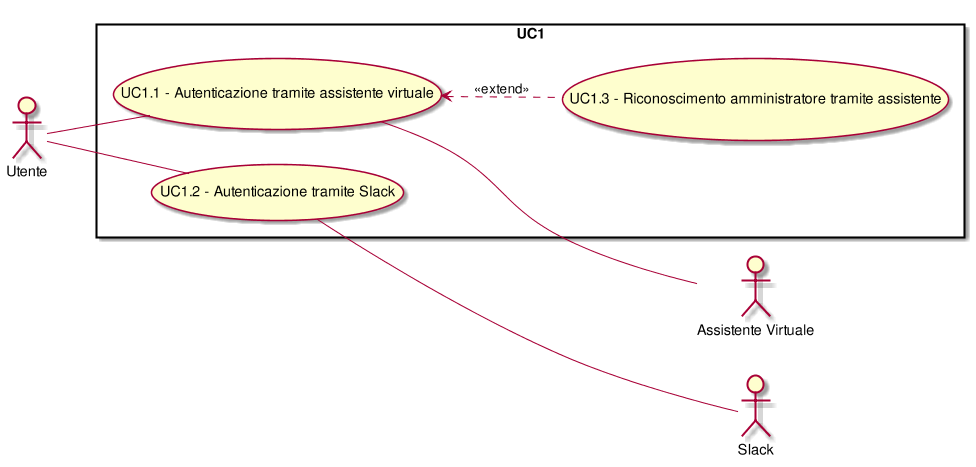
\includegraphics[width=\textwidth,height=\textheight,keepaspectratio]{images/UseCaseUC1.png}
\caption{UC1: Autenticazione}
\end{figure}
\begin{longtable}{l|p{10cm}}
\rowcolor[gray]{0.8} \multicolumn{2}{c}{} \\
\rowcolor[gray]{0.8} \multicolumn{2}{c}{\textbf{UC1 - Autenticazione}} \\
\rowcolor[gray]{0.8} \multicolumn{2}{c}{} \\
\hline
&\\
\textbf{Attori} & Utente.\\[7pt]
\textbf{Descrizione} & Il \gl{sistema} deve autenticare l'utente come ospite o come amministatore.\\[7pt]
\textbf{Precondizione} & Il sistema è stato avviato.\\[7pt]
\textbf{Postcondizione} & Il sitema ha riconosciuto l'utente come ospite o amministratore.\\[7pt]
\textbf{Scenario principale} &L'utente ha avviato il sistema per poter accedere alle funzionalità a lui dedicate.\\[7pt]\hline
\end{longtable}

\newpage\subsubsection{UC1.1: Autenticazione tramite assistente virtuale}
\label{UC1.1}
\begin{figure}[h]
\centering
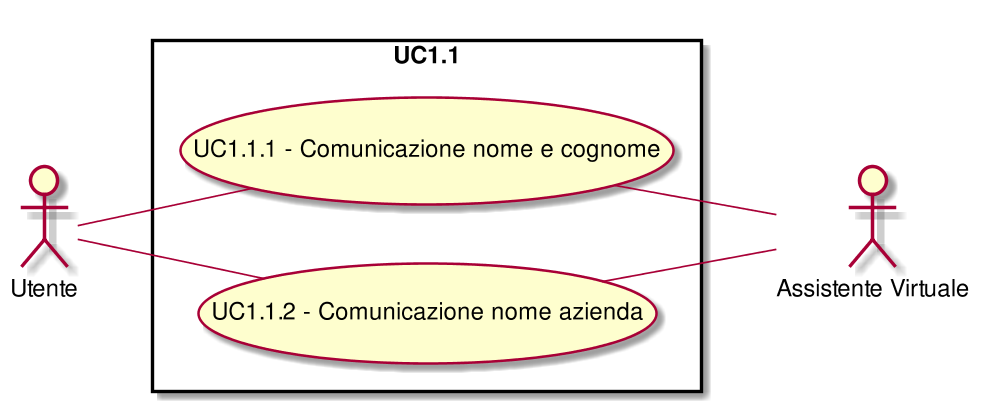
\includegraphics[width=\textwidth,height=\textheight,keepaspectratio]{images/UseCaseUC11.png}
\caption{UC1.1: Autenticazione tramite assistente virtuale}
\end{figure}
\begin{longtable}{l|p{10cm}}
\rowcolor[gray]{0.8} \multicolumn{2}{c}{} \\
\rowcolor[gray]{0.8} \multicolumn{2}{c}{\textbf{UC1.1 - Autenticazione tramite assistente virtuale}} \\
\rowcolor[gray]{0.8} \multicolumn{2}{c}{} \\
\hline
&\\
\textbf{Attori} & Assistente Virtuale, Utente.\\[7pt]
\textbf{Descrizione} & Il sistema può autenticare l'utente tramite l'assistente virtuale.\\[7pt]
\textbf{Precondizione} & L'utente utilizza direttamente l'assistente virtuale per la sua autenticazione.\\[7pt]
\textbf{Postcondizione} & Il sistema ha riconosciuto l'utente come ospite o amministratore.\\[7pt]
\textbf{Scenario principale} &L'utente viene autenticato tramite l'interazione con l'assistente virtuale.\\[7pt]
\textbf{Scenari alternativi} & Nel caso in cui nome e cognome dell'utente coincidano con quelli di un amministratore di sistema, l'assistente virtuale 
richiederà all'utente l'accesso all'area di amministrazione tramite riconoscimento vocale.\\[7pt]\hline
\end{longtable}

\newpage\subsubsection{UC1.1.1: Comunicazione nome e cognome}
\label{UC1.1.1}
\begin{longtable}{l|p{10cm}}
\rowcolor[gray]{0.8} \multicolumn{2}{c}{} \\
\rowcolor[gray]{0.8} \multicolumn{2}{c}{\textbf{UC1.1.1 - Comunicazione nome e cognome}} \\
\rowcolor[gray]{0.8} \multicolumn{2}{c}{} \\
\hline
&\\
\textbf{Attori} & Assistente Virtuale, Utente.\\[7pt]
\textbf{Descrizione} & Il sistema può richiedere all'ospite il proprio nome e cognome per poterlo autenticare.\\[7pt]
\textbf{Precondizione} & Il sistema ha chiesto all'ospite di comunicare il proprio nome e cognome.\\[7pt]
\textbf{Postcondizione} & Il sistema ha ricevuto il nome e cognome dell'ospite.\\[7pt]
\textbf{Scenario principale} &L'utente comunica al sistema il proprio nome e cognome. \\[7pt]\hline
\end{longtable}

\subsubsection{UC1.1.2: Comunicazione nome azienda}
\label{UC1.1.2}
\begin{longtable}{l|p{10cm}}
\rowcolor[gray]{0.8} \multicolumn{2}{c}{} \\
\rowcolor[gray]{0.8} \multicolumn{2}{c}{\textbf{UC1.1.2 - Comunicazione nome azienda}} \\
\rowcolor[gray]{0.8} \multicolumn{2}{c}{} \\
\hline
&\\
\textbf{Attori} & Assistente Virtuale, Utente.\\[7pt]
\textbf{Descrizione} & Il sistema può richiedere all'utente il nome dell'azienda da cui proviene.\\[7pt]
\textbf{Precondizione} & Il sistema ha richiesto all'utente l'azienda da cui proviene.\\[7pt]
\textbf{Postcondizione} & Il sistema ha ricevuto dall'utente il nome dell'azienda da cui proviene.\\[7pt]
\textbf{Scenario principale} &L'utente comunica il nome dell'azienda da cui proviene.\\[7pt]\hline
\end{longtable}

\subsubsection{UC1.2: Autenticazione tramite Slack}
\label{UC1.2}
\begin{longtable}{l|p{10cm}}
\rowcolor[gray]{0.8} \multicolumn{2}{c}{} \\
\rowcolor[gray]{0.8} \multicolumn{2}{c}{\textbf{UC1.2 - Autenticazione tramite Slack}} \\
\rowcolor[gray]{0.8} \multicolumn{2}{c}{} \\
\hline
&\\
\textbf{Attori} & Slack, Utente.\\[7pt]
\textbf{Descrizione} & Il sistema può permettere all'utente di identificarsi come amministratore tramite Slack.\\[7pt]
\textbf{Precondizione} & L'utente vuole autenticarsi come amministratore attraverso Slack.\\[7pt]
\textbf{Postcondizione} & Il sistema identifica l'utente come amministratore del sistema.\\[7pt]
\textbf{Scenario principale} &L'utente si identifica come amministratore tramite Slack.\\[7pt]\hline
\end{longtable}

\newpage\subsubsection{UC1.3: Riconoscimento amministratore tramite assistente}
\label{UC1.3}
\begin{figure}[h]
\centering
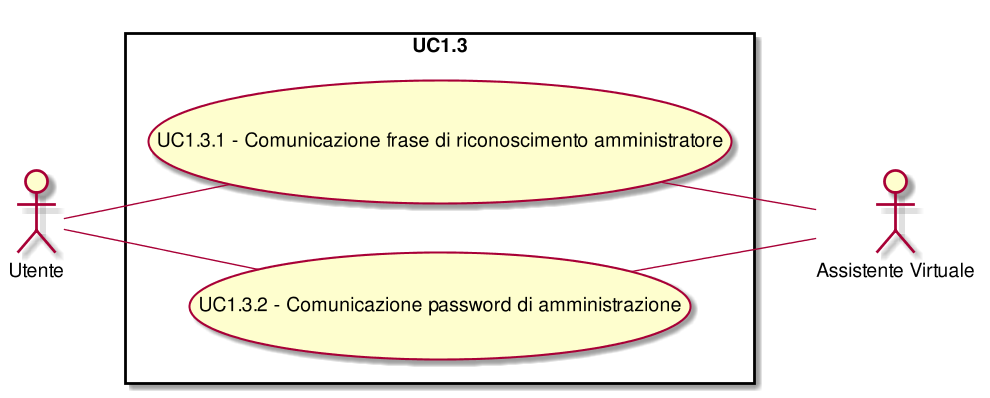
\includegraphics[width=\textwidth,height=\textheight,keepaspectratio]{images/UseCaseUC13.png}
\caption{UC1.3: Riconoscimento amministratore tramite assistente}
\end{figure}
\begin{longtable}{l|p{10cm}}
\rowcolor[gray]{0.8} \multicolumn{2}{c}{} \\
\rowcolor[gray]{0.8} \multicolumn{2}{c}{\textbf{UC1.3 - Riconoscimento amministratore tramite assistente}} \\
\rowcolor[gray]{0.8} \multicolumn{2}{c}{} \\
\hline
&\\
\textbf{Attori} & Assistente Virtuale, Utente.\\[7pt]
\textbf{Descrizione} & Il sistema offre all'utente la possibilità di autenticarsi come amministratore del sistema.\\[7pt]
\textbf{Precondizione} & Il sistema ha riconosciuto l'utente come possibile amministratore del sistema.\\[7pt]
\textbf{Postcondizione} & Il sistema ha autenticato l'utente come amministratore. \\[7pt]
\textbf{Scenario principale} &\begin{enumerate}
\item  L'utente può autenticarsi come amministratore attraverso la sua password;
\item  L'utente può autenticarsi come amministratore attraverso riconoscimento vocale.
\end{enumerate}
\\[7pt]\hline
\end{longtable}

\subsubsection{UC1.3.1: Comunicazione frase di riconoscimento amministratore}
\label{UC1.3.1}
\begin{longtable}{l|p{10cm}}
\rowcolor[gray]{0.8} \multicolumn{2}{c}{} \\
\rowcolor[gray]{0.8} \multicolumn{2}{c}{\textbf{UC1.3.1 - Comunicazione frase di riconoscimento amministratore}} \\
\rowcolor[gray]{0.8} \multicolumn{2}{c}{} \\
\hline
&\\
\textbf{Attori} & Assistente Virtuale, Utente.\\[7pt]
\textbf{Descrizione} & Il sistema può richiedere all'utente la frase necessaria per l'autenticazione come amministratore del sistema. \\[7pt]
\textbf{Precondizione} & Il sistema ha riconosciuto l'utente come uno dei possibili amministratori del sistema.\\[7pt]
\textbf{Postcondizione} & L'utente ha comunicato la frase necessaria per l'autenticazione come amministratore del sistema.\\[7pt]
\textbf{Scenario principale} &L'utente comunica la frase necessaria per l'autenticazione come amministratore del sistema. \\[7pt]
\textbf{Scenari alternativi} & Nel caso in cui la frase comunicata dall'utente non venga riconosciuta, il sistema richiederà nuovamente all'utente di pronunciarla.\\[7pt]\hline
\end{longtable}

\subsubsection{UC1.3.2: Comunicazione password di amministrazione}
\label{UC1.3.2}
\begin{longtable}{l|p{10cm}}
\rowcolor[gray]{0.8} \multicolumn{2}{c}{} \\
\rowcolor[gray]{0.8} \multicolumn{2}{c}{\textbf{UC1.3.2 - Comunicazione password di amministrazione}} \\
\rowcolor[gray]{0.8} \multicolumn{2}{c}{} \\
\hline
&\\
\textbf{Attori} & Assistente Virtuale, Utente.\\[7pt]
\textbf{Descrizione} & Il sistema offre all'utente la possibilità di autenticarsi come amministratore attraverso la sua password.\\[7pt]
\textbf{Precondizione} & Il sistema ha riconosciuto l'utente come possibile amministratore del sistema.\\[7pt]
\textbf{Postcondizione} & Il sistema ha autenticato l'utente come amministratore.\\[7pt]
\textbf{Scenario principale} &L'utente ha comunicato al sistema la sua password di amministrazione.\\[7pt]
\textbf{Scenari alternativi} & Nel caso in cui la password non sia corretta, il sistema la richiederà nuovamente.\\[7pt]\hline
\end{longtable}

\newpage\subsection{UC2: Accesso funzionalità amministratore}
\label{UC2}
\begin{figure}[h]
\centering
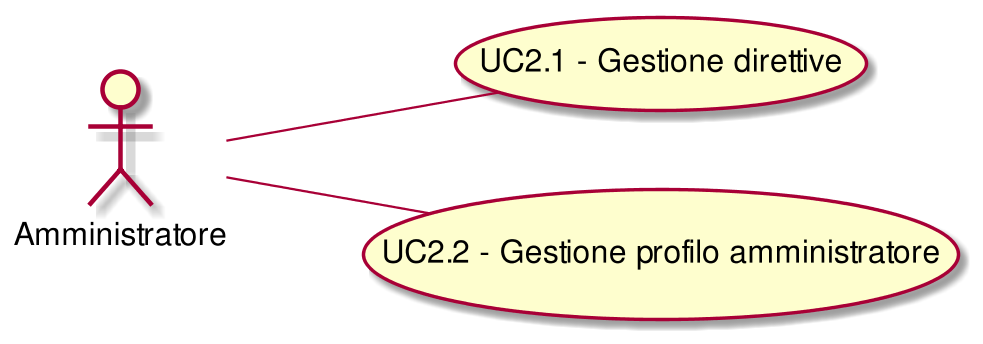
\includegraphics[width=\textwidth,height=\textheight,keepaspectratio]{images/UseCaseUC2.png}
\caption{UC2: Accesso funzionalità amministratore}
\end{figure}
\begin{longtable}{l|p{10cm}}
\rowcolor[gray]{0.8} \multicolumn{2}{c}{} \\
\rowcolor[gray]{0.8} \multicolumn{2}{c}{\textbf{UC2 - Accesso funzionalità amministratore}} \\
\rowcolor[gray]{0.8} \multicolumn{2}{c}{} \\
\hline
&\\
\textbf{Attori} & Amministratore.\\[7pt]
\textbf{Descrizione} & L'amministratore deve poter accedere alle funzionalità avanzate messe a disposizione dall'applicazione. Tali funzionalità consentono di fornire al sistema delle \gl{direttive} per modificare l'interazione con determinati ospiti.\\[7pt]
\textbf{Precondizione} & L'amministratore ha effettuato l'accesso all'area di amministrazione.\\[7pt]
\textbf{Postcondizione} & L'amministratore ha usufruito delle funzionalità di amministratore fornite dal sistema.\\[7pt]
\textbf{Scenario principale} &\begin{enumerate}
\item  L'amministratore può gestire le direttive del sistema da lui accessibili;
\item  L'amministratore può gestire le informazioni del proprio profilo.
\end{enumerate}
\\[7pt]\hline
\end{longtable}

\newpage\subsubsection{UC2.1: Gestione direttive}
\label{UC2.1}
\begin{figure}[h]
\centering
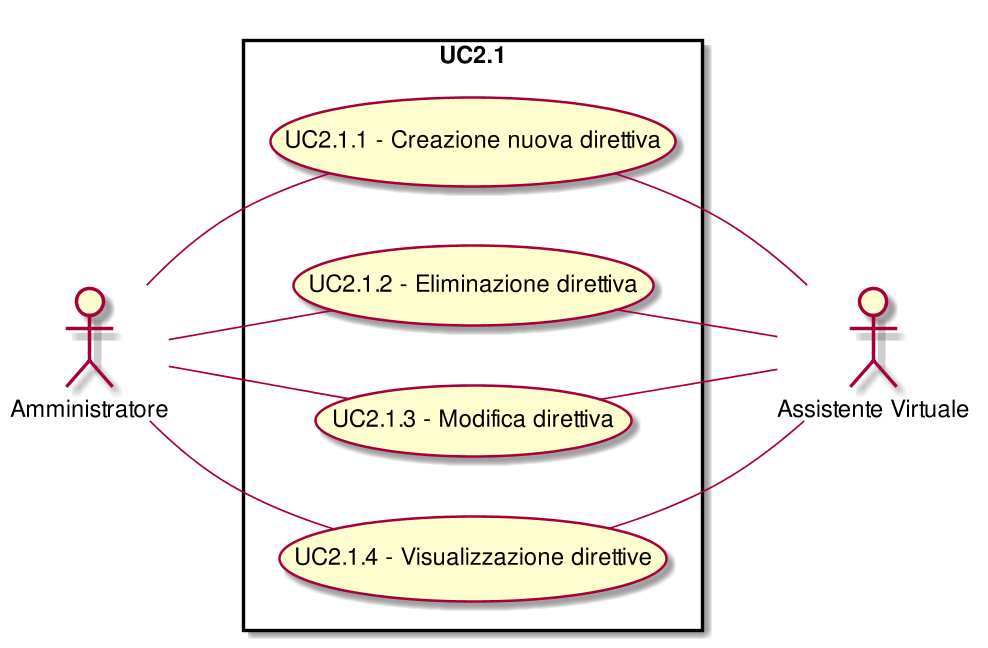
\includegraphics[width=\textwidth,height=\textheight,keepaspectratio]{images/UseCaseUC21.png}
\caption{UC2.1: Gestione direttive}
\end{figure}
\begin{longtable}{l|p{10cm}}
\rowcolor[gray]{0.8} \multicolumn{2}{c}{} \\
\rowcolor[gray]{0.8} \multicolumn{2}{c}{\textbf{UC2.1 - Gestione direttive}} \\
\rowcolor[gray]{0.8} \multicolumn{2}{c}{} \\
\hline
&\\
\textbf{Attori} & Amministratore, Assistente Virtuale.\\[7pt]
\textbf{Descrizione} & L'amministratore può creare nuove direttive o gestire quelle presenti nel sistema.\\[7pt]
\textbf{Precondizione} & L'amministratore si trova nella sezione adibita alla gestione delle direttive.\\[7pt]
\textbf{Postcondizione} & L'amministratore ha usufruito delle funzionalità di gestione delle direttive.\\[7pt]
\textbf{Scenario principale} &\begin{enumerate}
\item  L'amministratore può creare una nuova \gl{direttiva};
\item  L'amministratore può eliminare una direttiva di cui ha i privilegi;
\item  L'amministratore può modificare una direttiva di cui ha i privilegi;
\item  L'amministratore può ricercare le direttive di cui ha i privilegi secondo diversi criteri (nome, funzione, target e abilitazione).
\end{enumerate}
\\[7pt]\hline
\end{longtable}

\newpage\subsubsection{UC2.1.1: Creazione nuova direttiva}
\label{UC2.1.1}
\begin{figure}[h]
\centering
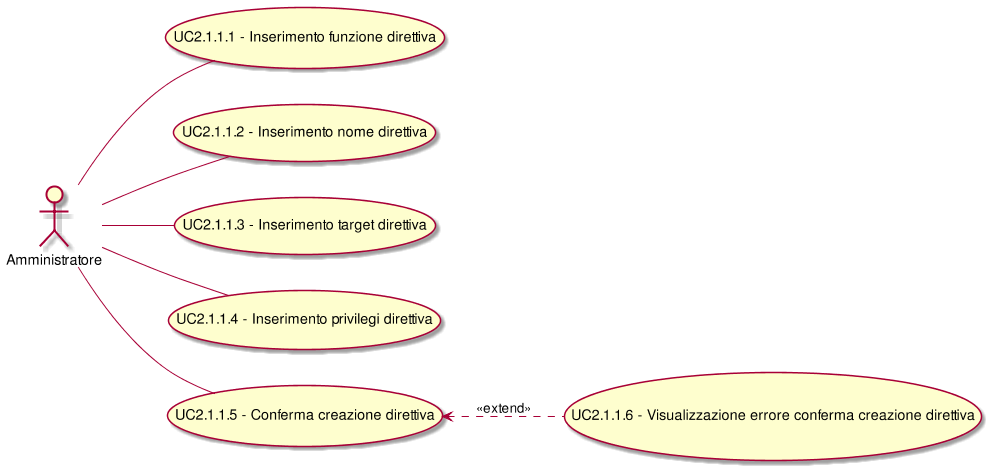
\includegraphics[width=\textwidth,height=\textheight,keepaspectratio]{images/UseCaseUC211.png}
\caption{UC2.1.1: Creazione nuova direttiva}
\end{figure}
\begin{longtable}{l|p{10cm}}
\rowcolor[gray]{0.8} \multicolumn{2}{c}{} \\
\rowcolor[gray]{0.8} \multicolumn{2}{c}{\textbf{UC2.1.1 - Creazione nuova direttiva}} \\
\rowcolor[gray]{0.8} \multicolumn{2}{c}{} \\
\hline
&\\
\textbf{Attori} & Amministratore, Assistente Virtuale.\\[7pt]
\textbf{Descrizione} & L'amministratore può creare una nuova direttiva, la quale sarà salvata nel sistema.\\[7pt]
\textbf{Precondizione} & L'amministratore si trova nella sezione dedicata alla creazione di una nuova direttiva.\\[7pt]
\textbf{Postcondizione} & La direttiva è stata creata e salvata nel sistema.\\[7pt]
\textbf{Scenario principale} &\begin{enumerate}
\item  L'amministratore può inserire il nome della direttiva;
\item  L'amministratore può inserire il target della direttiva;
\item  L'amministratore può inserire la funzione della direttiva;
\item  L'amministratore può confermare la creazione della direttiva. 
\end{enumerate}
\\[7pt]\hline
\end{longtable}

\newpage\subsubsection{UC2.1.1.1: Inserimento funzione direttiva}
\label{UC2.1.1.1}
\begin{longtable}{l|p{10cm}}
\rowcolor[gray]{0.8} \multicolumn{2}{c}{} \\
\rowcolor[gray]{0.8} \multicolumn{2}{c}{\textbf{UC2.1.1.1 - Inserimento funzione direttiva}} \\
\rowcolor[gray]{0.8} \multicolumn{2}{c}{} \\
\hline
&\\
\textbf{Attori} & Amministratore, Assistente Virtuale.\\[7pt]
\textbf{Descrizione} & L'amministratore può comunicare la funzione di una direttiva una volta richiesto dal sistema.\\[7pt]
\textbf{Precondizione} & Il sistema chiede all'amministratore la funzione della direttiva.\\[7pt]
\textbf{Postcondizione} & Il sistema ha ricevuto la funzione della direttiva.\\[7pt]
\textbf{Scenario principale} &L'amministratore comunica la funzione della direttiva.\\[7pt]\hline
\end{longtable}

\subsubsection{UC2.1.1.2: Inserimento nome direttiva}
\label{UC2.1.1.2}
\begin{longtable}{l|p{10cm}}
\rowcolor[gray]{0.8} \multicolumn{2}{c}{} \\
\rowcolor[gray]{0.8} \multicolumn{2}{c}{\textbf{UC2.1.1.2 - Inserimento nome direttiva}} \\
\rowcolor[gray]{0.8} \multicolumn{2}{c}{} \\
\hline
&\\
\textbf{Attori} & Amministratore, Assistente Virtuale.\\[7pt]
\textbf{Descrizione} & L'amministratore può comunicare il nome della direttiva una volta richiesto dal sistema.\\[7pt]
\textbf{Precondizione} & Il sistema ha richiesto il nome della direttiva all'amministratore.\\[7pt]
\textbf{Postcondizione} & Il sistema ha ricevuto il nome della direttiva.\\[7pt]
\textbf{Scenario principale} &L'amministratore comunica il nome della direttiva.\\[7pt]\hline
\end{longtable}

\newpage\subsubsection{UC2.1.1.3: Inserimento target direttiva}
\label{UC2.1.1.3}
\begin{figure}[h]
\centering
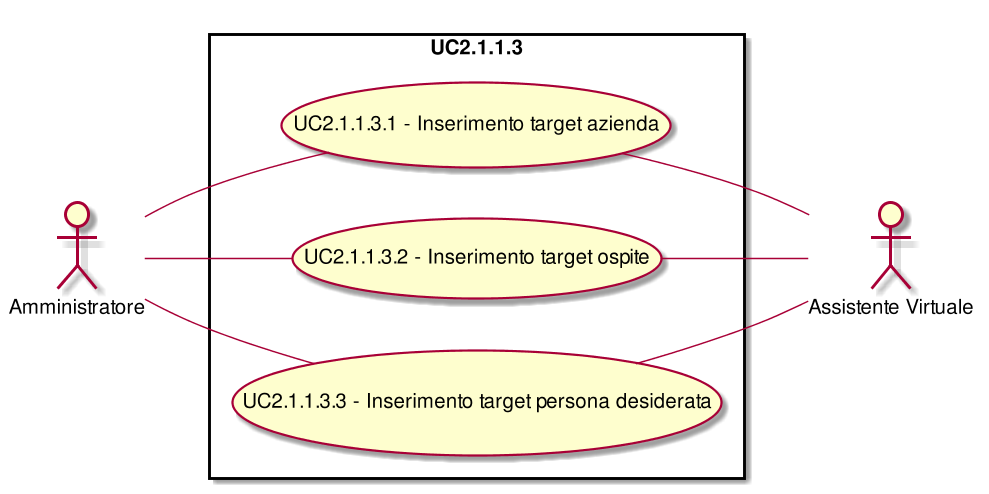
\includegraphics[width=\textwidth,height=\textheight,keepaspectratio]{images/UseCaseUC2113.png}
\caption{UC2.1.1.3: Inserimento target direttiva}
\end{figure}
\begin{longtable}{l|p{10cm}}
\rowcolor[gray]{0.8} \multicolumn{2}{c}{} \\
\rowcolor[gray]{0.8} \multicolumn{2}{c}{\textbf{UC2.1.1.3 - Inserimento target direttiva}} \\
\rowcolor[gray]{0.8} \multicolumn{2}{c}{} \\
\hline
&\\
\textbf{Attori} & Amministratore, Assistente Virtuale.\\[7pt]
\textbf{Descrizione} & L'amministratore può comunicare i target della direttiva, ovvero la categoria di persone a cui essa è rivolta, una volta richiesti dal sistema.\\[7pt]
\textbf{Precondizione} & Il sistema ha richiesto i target della direttiva all'amministratore.\\[7pt]
\textbf{Postcondizione} & Il sistema ha ricevuto i target della direttiva.\\[7pt]
\textbf{Scenario principale} &\begin{enumerate}
\item  L'amministratore può comunicare un'azienda come target;
\item  L'amministratore può comunicare il nome di un ospite come target;
\item  L'amministratore può comunicare una persona desiderata target.
\end{enumerate}
\\[7pt]\hline
\end{longtable}

\subsubsection{UC2.1.1.3.1: Inserimento target azienda}
\label{UC2.1.1.3.1}
\begin{longtable}{l|p{10cm}}
\rowcolor[gray]{0.8} \multicolumn{2}{c}{} \\
\rowcolor[gray]{0.8} \multicolumn{2}{c}{\textbf{UC2.1.1.3.1 - Inserimento target azienda}} \\
\rowcolor[gray]{0.8} \multicolumn{2}{c}{} \\
\hline
&\\
\textbf{Attori} & Amministratore, Assistente Virtuale.\\[7pt]
\textbf{Descrizione} & L'amministratore può comunicare il nome dell'azienda i cui dipendenti diventeranno i target della direttiva.\\[7pt]
\textbf{Precondizione} & Il sistema ha richiesto il nome dell'azienda target.\\[7pt]
\textbf{Postcondizione} & Il sistema ha ricevuto il nome dell'azienda target.\\[7pt]
\textbf{Scenario principale} &L'amministratore comunica il nome dell'azienda target.\\[7pt]\hline
\end{longtable}

\subsubsection{UC2.1.1.3.2: Inserimento target ospite}
\label{UC2.1.1.3.2}
\begin{longtable}{l|p{10cm}}
\rowcolor[gray]{0.8} \multicolumn{2}{c}{} \\
\rowcolor[gray]{0.8} \multicolumn{2}{c}{\textbf{UC2.1.1.3.2 - Inserimento target ospite}} \\
\rowcolor[gray]{0.8} \multicolumn{2}{c}{} \\
\hline
&\\
\textbf{Attori} & Amministratore, Assistente Virtuale.\\[7pt]
\textbf{Descrizione} & L'amministratore può comunicare il nome dell'ospite che diventerà il target della direttiva.\\[7pt]
\textbf{Precondizione} & Il sistema ha richiesto il nome dell'ospite target.\\[7pt]
\textbf{Postcondizione} & Il sistema ha ricevuto il nome dell'ospite target.\\[7pt]
\textbf{Scenario principale} &L'amministratore comunica il nome dell'ospite target.\\[7pt]\hline
\end{longtable}

\subsubsection{UC2.1.1.3.3: Inserimento target persona desiderata}
\label{UC2.1.1.3.3}
\begin{longtable}{l|p{10cm}}
\rowcolor[gray]{0.8} \multicolumn{2}{c}{} \\
\rowcolor[gray]{0.8} \multicolumn{2}{c}{\textbf{UC2.1.1.3.3 - Inserimento target persona desiderata}} \\
\rowcolor[gray]{0.8} \multicolumn{2}{c}{} \\
\hline
&\\
\textbf{Attori} & Amministratore, Assistente Virtuale.\\[7pt]
\textbf{Descrizione} & L'amministratore può comunicare il nome della persona desiderata. Tutti gli ospiti che vogliono incontrare questa persona diventeranno i target della direttiva.\\[7pt]
\textbf{Precondizione} & Il sistema ha richiesto il nome della persona desiderata.\\[7pt]
\textbf{Postcondizione} & Il sistema ha ricevuto il nome della persona desiderata.\\[7pt]
\textbf{Scenario principale} &L'amministratore comunica il nome della persona desiderata.\\[7pt]\hline
\end{longtable}

\subsubsection{UC2.1.1.4: Inserimento privilegi direttiva}
\label{UC2.1.1.4}
\begin{longtable}{l|p{10cm}}
\rowcolor[gray]{0.8} \multicolumn{2}{c}{} \\
\rowcolor[gray]{0.8} \multicolumn{2}{c}{\textbf{UC2.1.1.4 - Inserimento privilegi direttiva}} \\
\rowcolor[gray]{0.8} \multicolumn{2}{c}{} \\
\hline
&\\
\textbf{Attori} & Amministratore, Assistente Virtuale.\\[7pt]
\textbf{Descrizione} & L'amministratore può comunicare gli username degli amministratori a cui vuole concedere i privilegi di modifica ed eliminazione per la direttiva, una volta richiesti dal sistema.\\[7pt]
\textbf{Precondizione} & Il sistema ha richiesto gli username degli amministratori a cui l'amministratore vuole concedere i privilegi per la direttiva.\\[7pt]
\textbf{Postcondizione} & Il sistema ha ricevuto gli username comunicati dall'amministratore.\\[7pt]
\textbf{Scenario principale} &L'amministratore comunica gli username degli amministratori a cui vuole concedere i privilegi per la direttiva.\\[7pt]\hline
\end{longtable}

\subsubsection{UC2.1.1.5: Conferma creazione direttiva}
\label{UC2.1.1.5}
\begin{longtable}{l|p{10cm}}
\rowcolor[gray]{0.8} \multicolumn{2}{c}{} \\
\rowcolor[gray]{0.8} \multicolumn{2}{c}{\textbf{UC2.1.1.5 - Conferma creazione direttiva}} \\
\rowcolor[gray]{0.8} \multicolumn{2}{c}{} \\
\hline
&\\
\textbf{Attori} & Amministratore, Assistente Virtuale.\\[7pt]
\textbf{Descrizione} & L'amministratore può confermare i dati inseriti per creare una direttiva, una volta richiesto dal sistema.\\[7pt]
\textbf{Precondizione} & Il sistema chiede all'amministratore di confermare i dati comunicati.\\[7pt]
\textbf{Postcondizione} & Il sistema crea la direttiva con i dati comunicati dal sistema.\\[7pt]
\textbf{Scenario principale} &L'amministratore conferma di voler creare la nuova direttiva con i dati comunicati.\\[7pt]
\textbf{Scenari alternativi} & L'amministratore non conferma di voler creare la direttiva. L'amministratore viene rimandato alla pagina dedicata alla gestione delle direttive.\\[7pt]\hline
\end{longtable}

\subsubsection{UC2.1.1.6: Visualizzazione errore conferma creazione direttiva}
\label{UC2.1.1.6}
\begin{longtable}{l|p{10cm}}
\rowcolor[gray]{0.8} \multicolumn{2}{c}{} \\
\rowcolor[gray]{0.8} \multicolumn{2}{c}{\textbf{UC2.1.1.6 - Visualizzazione errore conferma creazione direttiva}} \\
\rowcolor[gray]{0.8} \multicolumn{2}{c}{} \\
\hline
&\\
\textbf{Attori} & Amministratore, Assistente Virtuale.\\[7pt]
\textbf{Descrizione} & L'amministratore può visualizzare un messaggio d'errore se ha comunicato dei dati non validi (funzione o target della direttiva inesistenti) per la creazione di una nuova direttiva.
\\[7pt]
\textbf{Precondizione} & Il sistema ha ricevuto dati non validi.\\[7pt]
\textbf{Postcondizione} & Il sistema mostra un messaggio d'errore adeguato.\\[7pt]
\textbf{Scenario principale} &L'amministratore visualizza un messaggio d'errore.\\[7pt]\hline
\end{longtable}

\newpage\subsubsection{UC2.1.2: Eliminazione direttiva }
\label{UC2.1.2}
\begin{figure}[h]
\centering

\includegraphics[width=\textwidth,height=\textheight,keepaspectratio]{images/UseCaseUC212.png}
\caption{UC2.1.2: Eliminazione direttiva }
\end{figure}
\begin{longtable}{l|p{10cm}}
\rowcolor[gray]{0.8} \multicolumn{2}{c}{} \\
\rowcolor[gray]{0.8} \multicolumn{2}{c}{\textbf{UC2.1.2 - Eliminazione direttiva }} \\
\rowcolor[gray]{0.8} \multicolumn{2}{c}{} \\
\hline
&\\
\textbf{Attori} & Amministratore, Assistente Virtuale.\\[7pt]
\textbf{Descrizione} & L'amministratore può eliminare dal sistema una direttiva di cui ha i privilegi. L'eliminazione comporterà la cancellazione dei dati dal sistema.\\[7pt]
\textbf{Precondizione} & Il sistema ha richesto all'amministratore la direttiva da eliminare.\\[7pt]
\textbf{Postcondizione} & Il sistema ha ricevuto i dati della direttiva da eliminare.\\[7pt]
\textbf{Scenario principale} &L'amministratore comunica i dati della direttiva da eliminare.\\[7pt]\hline
\end{longtable}

\subsubsection{UC2.1.2.1: Conferma eliminazione direttiva}
\label{UC2.1.2.1}
\begin{longtable}{l|p{10cm}}
\rowcolor[gray]{0.8} \multicolumn{2}{c}{} \\
\rowcolor[gray]{0.8} \multicolumn{2}{c}{\textbf{UC2.1.2.1 - Conferma eliminazione direttiva}} \\
\rowcolor[gray]{0.8} \multicolumn{2}{c}{} \\
\hline
&\\
\textbf{Attori} & Amministratore, Assistente Virtuale.\\[7pt]
\textbf{Descrizione} & L'amministratore può confermare l'eliminazione di una direttiva, una volta richiesto dal sistema.\\[7pt]
\textbf{Precondizione} & Il sistema ha richiesto all'amministratore la conferma della volontà di eliminare la direttiva.\\[7pt]
\textbf{Postcondizione} & L'amministratore ha eliminato una direttiva.\\[7pt]
\textbf{Scenario principale} &L'amministratore conferma di voler eliminare la direttiva.\\[7pt]
\textbf{Scenari alternativi} & L'amministratore non conferma di voler eliminare la direttiva. L'amministratore viene rimandato alla pagina dedicata alla gestione delle direttive.\\[7pt]\hline
\end{longtable}

\newpage\subsubsection{UC2.1.3: Modifica direttiva}
\label{UC2.1.3}
\begin{figure}[h]
\centering
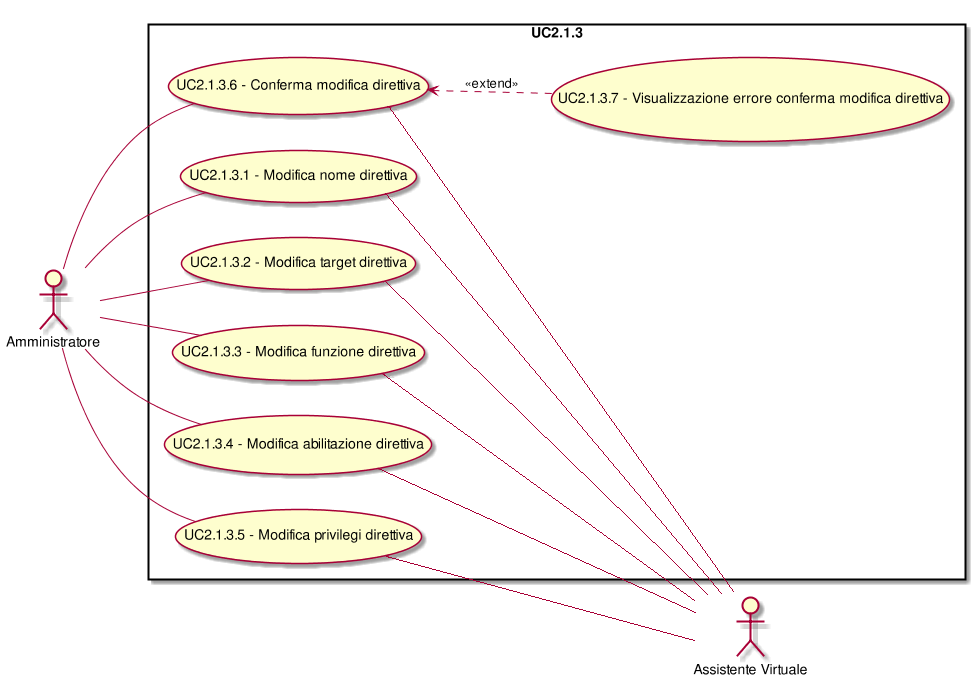
\includegraphics[width=\textwidth,height=\textheight,keepaspectratio]{images/UseCaseUC213.png}
\caption{UC2.1.3: Modifica direttiva}
\end{figure}
\begin{longtable}{l|p{10cm}}
\rowcolor[gray]{0.8} \multicolumn{2}{c}{} \\
\rowcolor[gray]{0.8} \multicolumn{2}{c}{\textbf{UC2.1.3 - Modifica direttiva}} \\
\rowcolor[gray]{0.8} \multicolumn{2}{c}{} \\
\hline
&\\
\textbf{Attori} & Amministratore, Assistente Virtuale.\\[7pt]
\textbf{Descrizione} & L'amministratore può modificare una direttiva di cui ha i privilegi. \\[7pt]
\textbf{Precondizione} & Il sistema ha richiesto all'amministratore di modificare una direttiva.\\[7pt]
\textbf{Postcondizione} & Il sistema ha modificato la direttiva in base ai dati comunicati dall'amministratore.\\[7pt]
\textbf{Scenario principale} &\begin{enumerate}
\item  L'amministratore può modificare il nome della direttiva;
\item  L'amministratore può modificare il target della direttiva;
\item  L'amministratore può modificare la funzione della direttiva;
\item  L'amministratore può abilitare o disabilitare una direttiva;
\item  L'amministratore può confermare le modifiche apportate alla direttiva.
\end{enumerate}
\\[7pt]\hline
\end{longtable}

\newpage\subsubsection{UC2.1.3.1: Modifica nome direttiva}
\label{UC2.1.3.1}
\begin{longtable}{l|p{10cm}}
\rowcolor[gray]{0.8} \multicolumn{2}{c}{} \\
\rowcolor[gray]{0.8} \multicolumn{2}{c}{\textbf{UC2.1.3.1 - Modifica nome direttiva}} \\
\rowcolor[gray]{0.8} \multicolumn{2}{c}{} \\
\hline
&\\
\textbf{Attori} & Amministratore, Assistente Virtuale.\\[7pt]
\textbf{Descrizione} & L'amministratore può comunicare il nuovo nome di una direttiva.\\[7pt]
\textbf{Precondizione} & Il sistema ha chiesto all'amministratore il nuovo nome della direttiva.\\[7pt]
\textbf{Postcondizione} & Il sistema ha ricevuto i dati dall'amministratore per modificare il nome di una direttiva.\\[7pt]
\textbf{Scenario principale} &L'amministratore comunica il nuovo nome per una direttiva.\\[7pt]\hline
\end{longtable}

\newpage\subsubsection{UC2.1.3.2: Modifica target direttiva}
\label{UC2.1.3.2}
\begin{figure}[h]
\centering
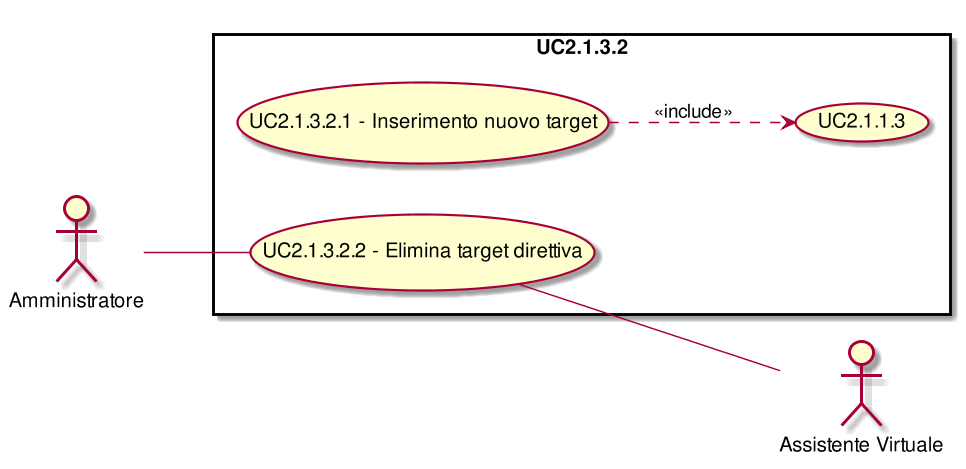
\includegraphics[width=\textwidth,height=\textheight,keepaspectratio]{images/UseCaseUC2132.png}
\caption{UC2.1.3.2: Modifica target direttiva}
\end{figure}
\begin{longtable}{l|p{10cm}}
\rowcolor[gray]{0.8} \multicolumn{2}{c}{} \\
\rowcolor[gray]{0.8} \multicolumn{2}{c}{\textbf{UC2.1.3.2 - Modifica target direttiva}} \\
\rowcolor[gray]{0.8} \multicolumn{2}{c}{} \\
\hline
&\\
\textbf{Attori} & Amministratore, Assistente Virtuale.\\[7pt]
\textbf{Descrizione} & L'amministratore può comunicare i dati per modiifcare i target di una direttiva.\\[7pt]
\textbf{Precondizione} & Il sistema ha chiesto all'amministratore il nuovo target della direttiva.\\[7pt]
\textbf{Postcondizione} & Il sistema ha ricevuto i dati dall'amministratore per modificare il target di una direttiva.\\[7pt]
\textbf{Scenario principale} &\begin{enumerate}
\item  L'amministratore può comunicare i dati per aggiungere un nuovo target alla direttiva;
\item  L'amministratore può comunicare i dati per eliminare un target dalla direttiva.
\end{enumerate}
\\[7pt]\hline
\end{longtable}

\newpage\subsubsection{UC2.1.3.2.1: Inserimento nuovo target}
\label{UC2.1.3.2.1}
\begin{longtable}{l|p{10cm}}
\rowcolor[gray]{0.8} \multicolumn{2}{c}{} \\
\rowcolor[gray]{0.8} \multicolumn{2}{c}{\textbf{UC2.1.3.2.1 - Inserimento nuovo target}} \\
\rowcolor[gray]{0.8} \multicolumn{2}{c}{} \\
\hline
&\\
\textbf{Attori} & Amministratore, Assistente Virtuale.\\[7pt]
\textbf{Descrizione} & L'amministratore può aggiungere un target alla direttiva.\\[7pt]
\textbf{Precondizione} & Il sistema ha chiesto all'amministratore il nuovo target della direttiva.\\[7pt]
\textbf{Postcondizione} & Il sistema ha ricevuto dall'amministratore il nuovo target della direttiva.\\[7pt]
\textbf{Scenario principale} &L'amministratore comunica il nuovo target della direttiva.\\[7pt]
\textbf{Inclusioni} & UC2.1.1.3\\[7pt]\hline
\end{longtable}

\subsubsection{UC2.1.3.2.2: Elimina target direttiva}
\label{UC2.1.3.2.2}
\begin{longtable}{l|p{10cm}}
\rowcolor[gray]{0.8} \multicolumn{2}{c}{} \\
\rowcolor[gray]{0.8} \multicolumn{2}{c}{\textbf{UC2.1.3.2.2 - Elimina target direttiva}} \\
\rowcolor[gray]{0.8} \multicolumn{2}{c}{} \\
\hline
&\\
\textbf{Attori} & Amministratore, Assistente Virtuale.\\[7pt]
\textbf{Descrizione} & L'amministratore può eliminare un target della direttiva.\\[7pt]
\textbf{Precondizione} & Il sistema ha chiesto all'amministratore il target da eliminare della direttiva interessata.\\[7pt]
\textbf{Postcondizione} & Il sistema ha ricevuto dall'amministratore il target da eliminare della direttiva interessata.\\[7pt]
\textbf{Scenario principale} &Il sistema riceve dall'amministratore il target da eliminare della direttiva interessata.\\[7pt]\hline
\end{longtable}

\subsubsection{UC2.1.3.3: Modifica funzione direttiva}
\label{UC2.1.3.3}
\begin{longtable}{l|p{10cm}}
\rowcolor[gray]{0.8} \multicolumn{2}{c}{} \\
\rowcolor[gray]{0.8} \multicolumn{2}{c}{\textbf{UC2.1.3.3 - Modifica funzione direttiva}} \\
\rowcolor[gray]{0.8} \multicolumn{2}{c}{} \\
\hline
&\\
\textbf{Attori} & Amministratore, Assistente Virtuale.\\[7pt]
\textbf{Descrizione} & L'amministratore può comunicare i dati per modificare la funzione di una direttiva.\\[7pt]
\textbf{Precondizione} & Il sistema ha chiesto all'amministratore la nuova funzione della direttiva.\\[7pt]
\textbf{Postcondizione} & Il sistema ha ricevuto i dati dall'amministratore per modificare la funzione di una direttiva.\\[7pt]
\textbf{Scenario principale} &L'amministratore comunica i dati per modificare la funzione di una direttiva.\\[7pt]\hline
\end{longtable}

\subsubsection{UC2.1.3.4: Modifica abilitazione direttiva}
\label{UC2.1.3.4}
\begin{longtable}{l|p{10cm}}
\rowcolor[gray]{0.8} \multicolumn{2}{c}{} \\
\rowcolor[gray]{0.8} \multicolumn{2}{c}{\textbf{UC2.1.3.4 - Modifica abilitazione direttiva}} \\
\rowcolor[gray]{0.8} \multicolumn{2}{c}{} \\
\hline
&\\
\textbf{Attori} & Amministratore, Assistente Virtuale.\\[7pt]
\textbf{Descrizione} & L'amministratore può comunicare i dati per modificare l'abilitazione di una direttiva.\\[7pt]
\textbf{Precondizione} & Il sistema ha chiesto all'amministratore come vuole modificare l'abilitazione della direttiva.\\[7pt]
\textbf{Postcondizione} & Il sistema ha ricevuto i dati dall'amministratore per modificare l'abilitazione di una direttiva.\\[7pt]
\textbf{Scenario principale} &L'amministratore comunica i dati per modificare l'abilitazione di una direttiva.\\[7pt]\hline
\end{longtable}

\newpage\subsubsection{UC2.1.3.5: Modifica privilegi direttiva}
\label{UC2.1.3.5}
\begin{figure}[h]
\centering
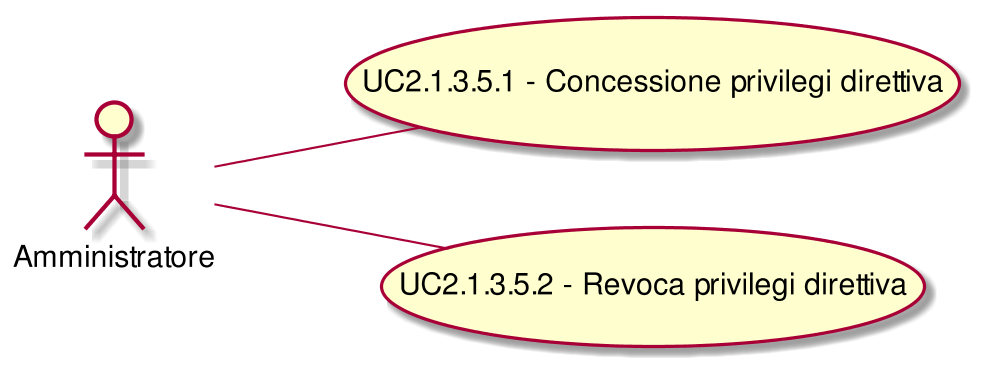
\includegraphics[width=\textwidth,height=\textheight,keepaspectratio]{images/UseCaseUC2135.png}
\caption{UC2.1.3.5: Modifica privilegi direttiva}
\end{figure}
\begin{longtable}{l|p{10cm}}
\rowcolor[gray]{0.8} \multicolumn{2}{c}{} \\
\rowcolor[gray]{0.8} \multicolumn{2}{c}{\textbf{UC2.1.3.5 - Modifica privilegi direttiva}} \\
\rowcolor[gray]{0.8} \multicolumn{2}{c}{} \\
\hline
&\\
\textbf{Attori} & Amministratore, Assistente Virtuale.\\[7pt]
\textbf{Descrizione} & L'amministratore può comunicare la volontà di modificare i privilegi per una direttiva.\\[7pt]
\textbf{Precondizione} & Il sistema ha chiesto all'amministratore se vuole modificare i privilegi di altri amministratori per la direttiva.\\[7pt]
\textbf{Postcondizione} & Il sistema ha ricevuto i dati dall'amministratore per modificare i privilegi degli altri amministratori per la direttiva.\\[7pt]
\textbf{Scenario principale} &\begin{enumerate}
\item  L'amministratore può concedere ad un altro amministratore i privilegi per una direttiva;
\item  L'amministratore può revocare i privilegi di un altro amministratore per una direttiva.
\end{enumerate}
\\[7pt]\hline
\end{longtable}

\subsubsection{UC2.1.3.5.1: Concessione privilegi direttiva}
\label{UC2.1.3.5.1}
\begin{longtable}{l|p{10cm}}
\rowcolor[gray]{0.8} \multicolumn{2}{c}{} \\
\rowcolor[gray]{0.8} \multicolumn{2}{c}{\textbf{UC2.1.3.5.1 - Concessione privilegi direttiva}} \\
\rowcolor[gray]{0.8} \multicolumn{2}{c}{} \\
\hline
&\\
\textbf{Attori} & Amministratore, Assistente Virtuale.\\[7pt]
\textbf{Descrizione} & L'amministratore può comunicare i dati per concedere ad altri amministratori i privilegi per la direttiva. L'altro amministratore in seguito potrà visualizzare, modificare ed eliminare la direttiva.\\[7pt]
\textbf{Precondizione} & Il sistema ha chiesto all'amministratore a quali altri amministratori vuole estendere i privilegi per la direttiva.\\[7pt]
\textbf{Postcondizione} & Il sistema ha ricevuto i dati dall'amministratore per concedere i privilegi di una direttiva ad ulteriori amministratori.\\[7pt]
\textbf{Scenario principale} &L'amministratore comunica i dati per concedere i privilegi per la direttiva ad altri amministratori.\\[7pt]\hline
\end{longtable}

\subsubsection{UC2.1.3.5.2: Revoca privilegi direttiva}
\label{UC2.1.3.5.2}
\begin{longtable}{l|p{10cm}}
\rowcolor[gray]{0.8} \multicolumn{2}{c}{} \\
\rowcolor[gray]{0.8} \multicolumn{2}{c}{\textbf{UC2.1.3.5.2 - Revoca privilegi direttiva}} \\
\rowcolor[gray]{0.8} \multicolumn{2}{c}{} \\
\hline
&\\
\textbf{Attori} & Amministratore, Assistente Virtuale.\\[7pt]
\textbf{Descrizione} & L'amministratore può revocare i privilegi degli altri amministratori per la direttiva.\\[7pt]
\textbf{Precondizione} & Il sistema ha chiesto all'amministratore a quali amministratori vuole revocare i privilegi per la direttiva.\\[7pt]
\textbf{Postcondizione} & Il sistema ha ricevuto gli username degli amministratori ai quali devono essere revocati i privilegi per la direttiva.\\[7pt]
\textbf{Scenario principale} &L'amministratore comunica gli username degli amministratori ai quali devono essere revocati i privilegi per la direttiva.\\[7pt]\hline
\end{longtable}

\subsubsection{UC2.1.3.6: Conferma modifica direttiva}
\label{UC2.1.3.6}
\begin{longtable}{l|p{10cm}}
\rowcolor[gray]{0.8} \multicolumn{2}{c}{} \\
\rowcolor[gray]{0.8} \multicolumn{2}{c}{\textbf{UC2.1.3.6 - Conferma modifica direttiva}} \\
\rowcolor[gray]{0.8} \multicolumn{2}{c}{} \\
\hline
&\\
\textbf{Attori} & Amministratore, Assistente Virtuale.\\[7pt]
\textbf{Descrizione} & L'amministratore può confermare la modifica di una direttiva.\\[7pt]
\textbf{Precondizione} & Il sistema ha richiesto all'amministratore la conferma delle modifiche alla direttiva.\\[7pt]
\textbf{Postcondizione} & Il sistema ha ricevuto la conferma da parte dell'amministratore.\\[7pt]
\textbf{Scenario principale} &L'amministratore conferma di voler modificare una direttiva.\\[7pt]
\textbf{Scenari alternativi} & L'amministratore non conferma di voler modificare la direttiva. L'amministratore viene rimandato alla pagina dedicata alla gestione delle direttive.\\[7pt]\hline
\end{longtable}

\newpage\subsubsection{UC2.1.3.7: Visualizzazione errore conferma modifica direttiva}
\label{UC2.1.3.7}
\begin{longtable}{l|p{10cm}}
\rowcolor[gray]{0.8} \multicolumn{2}{c}{} \\
\rowcolor[gray]{0.8} \multicolumn{2}{c}{\textbf{UC2.1.3.7 - Visualizzazione errore conferma modifica direttiva}} \\
\rowcolor[gray]{0.8} \multicolumn{2}{c}{} \\
\hline
&\\
\textbf{Attori} & Amministratore, Assistente Virtuale.\\[7pt]
\textbf{Descrizione} & L'amministratore può visualizzare un messaggio d'errore se ha comunicato dei dati non validi (target o funzione inesistenti) per la modifica di una direttiva.
\\[7pt]
\textbf{Precondizione} & Il sistema ha ricevuto dati non validi.\\[7pt]
\textbf{Postcondizione} & Il sistema mostra un messaggio d'errore.\\[7pt]
\textbf{Scenario principale} &L'amministratore visualizza un messaggio d'errore.\\[7pt]\hline
\end{longtable}

\subsubsection{UC2.1.4: Visualizzazione direttive }
\label{UC2.1.4}
\begin{longtable}{l|p{10cm}}
\rowcolor[gray]{0.8} \multicolumn{2}{c}{} \\
\rowcolor[gray]{0.8} \multicolumn{2}{c}{\textbf{UC2.1.4 - Visualizzazione direttive }} \\
\rowcolor[gray]{0.8} \multicolumn{2}{c}{} \\
\hline
&\\
\textbf{Attori} & Amministratore, Assistente Virtuale.\\[7pt]
\textbf{Descrizione} & L'amministratore può visualizzare tutte le direttive per le quali detiene i privilegi.\\[7pt]
\textbf{Precondizione} & L'amministratore si trova nella sezione dedicata alla visualizzazione delle direttive.\\[7pt]
\textbf{Postcondizione} & L'amministratore ha visualizzato le direttive di cui detiene i privilegi.\\[7pt]
\textbf{Scenario principale} &L'amministratore visualizza tutte le direttive di cui detiene i privilegi.\\[7pt]\hline
\end{longtable}

\newpage\subsubsection{UC2.2: Gestione profilo amministratore}
\label{UC2.2}
\begin{figure}[h]
\centering
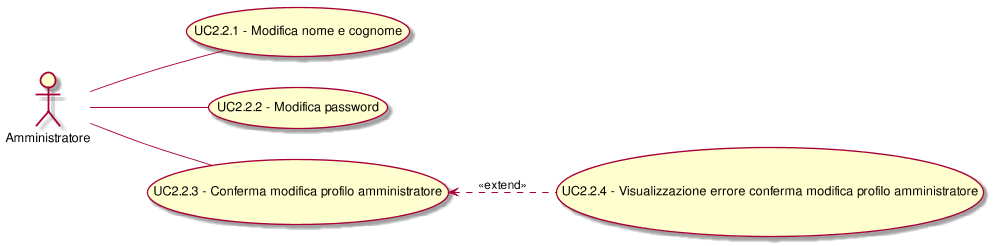
\includegraphics[width=\textwidth,height=\textheight,keepaspectratio]{images/UseCaseUC22.png}
\caption{UC2.2: Gestione profilo amministratore}
\end{figure}
\begin{longtable}{l|p{10cm}}
\rowcolor[gray]{0.8} \multicolumn{2}{c}{} \\
\rowcolor[gray]{0.8} \multicolumn{2}{c}{\textbf{UC2.2 - Gestione profilo amministratore}} \\
\rowcolor[gray]{0.8} \multicolumn{2}{c}{} \\
\hline
&\\
\textbf{Attori} & Amministratore, Assistente Virtuale.\\[7pt]
\textbf{Descrizione} & L'amministratore può gestire le impostazioni del proprio profilo tramite le funzionalità  offerte dal sistema.\\[7pt]
\textbf{Precondizione} & L'amministratore si trova nella sezione adibita alla gestione delle impostazioni del proprio profilo.\\[7pt]
\textbf{Postcondizione} & L'amministratore ha usufruito delle funzionalità per gestire le impostazioni del proprio profilo.\\[7pt]
\textbf{Scenario principale} &\begin{enumerate}
\item  L'amministratore può modificare il proprio nome e cognome;
\item  L'amministratore può modificare la propria password;
\item  L'amministratore può confermare le modifiche effettuate.
\end{enumerate}
\\[7pt]\hline
\end{longtable}

\subsubsection{UC2.2.1: Modifica nome e cognome}
\label{UC2.2.1}
\begin{longtable}{l|p{10cm}}
\rowcolor[gray]{0.8} \multicolumn{2}{c}{} \\
\rowcolor[gray]{0.8} \multicolumn{2}{c}{\textbf{UC2.2.1 - Modifica nome e cognome}} \\
\rowcolor[gray]{0.8} \multicolumn{2}{c}{} \\
\hline
&\\
\textbf{Attori} & Amministratore, Assistente Virtuale.\\[7pt]
\textbf{Descrizione} & L'amministratore può modificare il nome e cognome del suo profilo.\\[7pt]
\textbf{Precondizione} & L'amministratore si trova nella sezione dedicata alla modifica del nome e del cognome del suo profilo.\\[7pt]
\textbf{Postcondizione} & L'amministratore ha modificato il nome e cognome del suo profilo.\\[7pt]
\textbf{Scenario principale} &L'amministratore modifica il nome e cognome del suo profilo.\\[7pt]\hline
\end{longtable}

\newpage\subsubsection{UC2.2.2: Modifica password}
\label{UC2.2.2}
\begin{figure}[h]
\centering
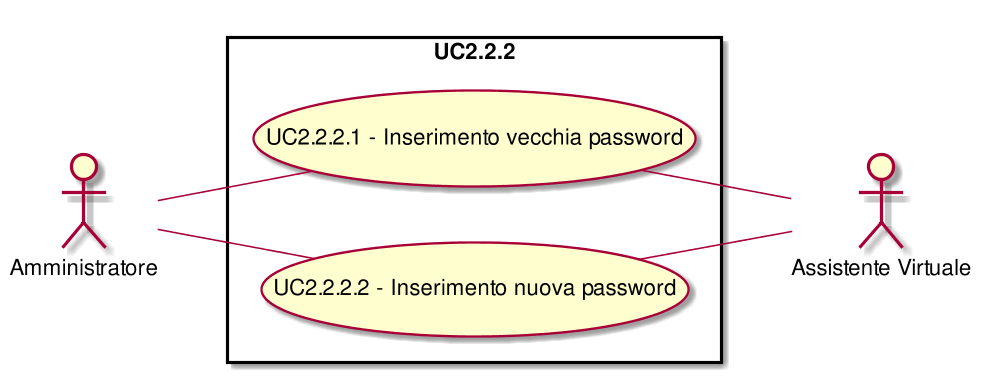
\includegraphics[width=\textwidth,height=\textheight,keepaspectratio]{images/UseCaseUC222.png}
\caption{UC2.2.2: Modifica password}
\end{figure}
\begin{longtable}{l|p{10cm}}
\rowcolor[gray]{0.8} \multicolumn{2}{c}{} \\
\rowcolor[gray]{0.8} \multicolumn{2}{c}{\textbf{UC2.2.2 - Modifica password}} \\
\rowcolor[gray]{0.8} \multicolumn{2}{c}{} \\
\hline
&\\
\textbf{Attori} & Amministratore, Assistente Virtuale.\\[7pt]
\textbf{Descrizione} & L'amministratore può modificare la password del suo profilo.\\[7pt]
\textbf{Precondizione} & L'amministratore si trova nella sezione dedicata alla modifica della password del suo profilo.\\[7pt]
\textbf{Postcondizione} & L'amministratore ha modificato la password del suo profilo.\\[7pt]
\textbf{Scenario principale} &\begin{enumerate}
\item  L'attore può inserire la propria vecchia password;
\item  L'attore può inserire una nuova password.
\end{enumerate}
\\[7pt]
\textbf{Scenari alternativi} & L'amministratore non conferma di voler modificare la propria password. L'amministratore viene rimandato alla pagina dedicata alla gestione delle direttive.\\[7pt]\hline
\end{longtable}

\subsubsection{UC2.2.2.1: Inserimento vecchia password}
\label{UC2.2.2.1}
\begin{longtable}{l|p{10cm}}
\rowcolor[gray]{0.8} \multicolumn{2}{c}{} \\
\rowcolor[gray]{0.8} \multicolumn{2}{c}{\textbf{UC2.2.2.1 - Inserimento vecchia password}} \\
\rowcolor[gray]{0.8} \multicolumn{2}{c}{} \\
\hline
&\\
\textbf{Attori} & Amministratore, Assistente Virtuale.\\[7pt]
\textbf{Descrizione} & L'amministratore può inserire la vecchia password.\\[7pt]
\textbf{Precondizione} & L'amministratore si trova nella sezione dedicata all'inserimento della vecchia password.\\[7pt]
\textbf{Postcondizione} & L'amministratore ha inserito la vecchia password.\\[7pt]
\textbf{Scenario principale} &L'amministratore inserisce la vecchia password.\\[7pt]\hline
\end{longtable}

\subsubsection{UC2.2.2.2: Inserimento nuova password}
\label{UC2.2.2.2}
\begin{longtable}{l|p{10cm}}
\rowcolor[gray]{0.8} \multicolumn{2}{c}{} \\
\rowcolor[gray]{0.8} \multicolumn{2}{c}{\textbf{UC2.2.2.2 - Inserimento nuova password}} \\
\rowcolor[gray]{0.8} \multicolumn{2}{c}{} \\
\hline
&\\
\textbf{Attori} & Amministratore, Assistente Virtuale.\\[7pt]
\textbf{Descrizione} & L'amministratore può inserire la nuova password.\\[7pt]
\textbf{Precondizione} & L'amministratore si trova nella sezione dedicata all'inserimento di una nuova password.\\[7pt]
\textbf{Postcondizione} & L'amministratore ha inserito la nuova password.\\[7pt]
\textbf{Scenario principale} &L'amministratore inserisce la nuova password.\\[7pt]\hline
\end{longtable}

\subsubsection{UC2.2.3: Conferma modifica profilo amministratore}
\label{UC2.2.3}
\begin{longtable}{l|p{10cm}}
\rowcolor[gray]{0.8} \multicolumn{2}{c}{} \\
\rowcolor[gray]{0.8} \multicolumn{2}{c}{\textbf{UC2.2.3 - Conferma modifica profilo amministratore}} \\
\rowcolor[gray]{0.8} \multicolumn{2}{c}{} \\
\hline
&\\
\textbf{Attori} & Amministratore, Assistente Virtuale.\\[7pt]
\textbf{Descrizione} & L'amministratore può confermare le modifiche al profilo.\\[7pt]
\textbf{Precondizione} & L'amministratore ha inserito i dati necessari alla modifica del profilo.\\[7pt]
\textbf{Postcondizione} & L'amministratore ha modificato il profilo.\\[7pt]
\textbf{Scenario principale} &L'amministratore modifica il profilo.\\[7pt]
\textbf{Scenari alternativi} & L'amministratore può non confermare le modifiche al profilo. Viene quindi rimandato alla pagina principale delle funzionalità di un amministratore.\\[7pt]\hline
\end{longtable}

\subsubsection{UC2.2.4: Visualizzazione errore conferma modifica profilo amministratore }
\label{UC2.2.4}
\begin{longtable}{l|p{10cm}}
\rowcolor[gray]{0.8} \multicolumn{2}{c}{} \\
\rowcolor[gray]{0.8} \multicolumn{2}{c}{\textbf{UC2.2.4 - Visualizzazione errore conferma modifica profilo amministratore }} \\
\rowcolor[gray]{0.8} \multicolumn{2}{c}{} \\
\hline
&\\
\textbf{Attori} & Amministratore, Assistente Virtuale.\\[7pt]
\textbf{Descrizione} & L'amministratore può visualizzare un messaggio d'errore se ha comunicato dei dati non validi per la modifica del profilo d'amministratore.
I dati non validi sono: username già esistente o la vecchia password non coincide con quella attuale.\\[7pt]
\textbf{Precondizione} & Il sistema ha ricevuto dati non validi.\\[7pt]
\textbf{Postcondizione} & Il sistema mostra un messaggio d'errore.\\[7pt]
\textbf{Scenario principale} &L'amministratore visualizza un messaggio d'errore.\\[7pt]\hline
\end{longtable}

\newpage\subsection{UC3: Accoglienza ospite}
\label{UC3}
\begin{figure}[h]
\centering
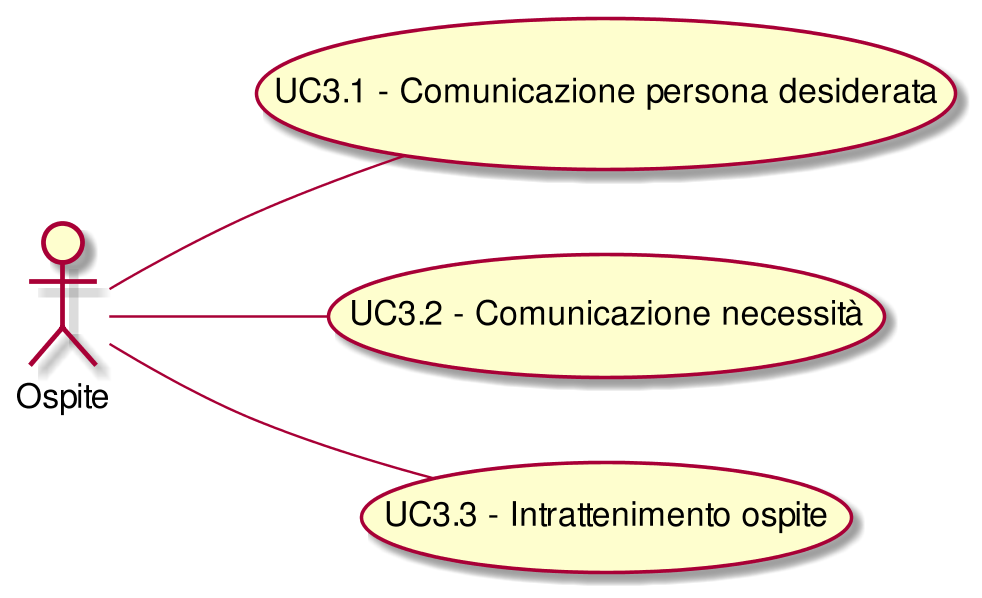
\includegraphics[width=\textwidth,height=\textheight,keepaspectratio]{images/UseCaseUC3.png}
\caption{UC3: Accoglienza ospite}
\end{figure}
\begin{longtable}{l|p{10cm}}
\rowcolor[gray]{0.8} \multicolumn{2}{c}{} \\
\rowcolor[gray]{0.8} \multicolumn{2}{c}{\textbf{UC3 - Accoglienza ospite}} \\
\rowcolor[gray]{0.8} \multicolumn{2}{c}{} \\
\hline
&\\
\textbf{Attori} & Ospite.\\[7pt]
\textbf{Descrizione} & L'ospite può essere accolto dal sistema tramite le funzionalità da esso offerte.\\[7pt]
\textbf{Precondizione} & Il sistema ha riconosciuto l'utente come ospite dell'azienda.\\[7pt]
\textbf{Postcondizione} & L'ospite è stato accolto usufruendo delle funzionalità del sistema.\\[7pt]
\textbf{Scenario principale} &\begin{enumerate}
\item  L'ospite può comunicare la persona desiderata per il suo incontro;
\item  L'ospite può esprimere alcune necessità  particolari riguardanti l'incontro;
\item  L'ospite può essere intrattenuto dal sistema durante l'attesa.
\end{enumerate}
\\[7pt]\hline
\end{longtable}

\newpage\subsubsection{UC3.1: Comunicazione persona desiderata}
\label{UC3.1}
\begin{longtable}{l|p{10cm}}
\rowcolor[gray]{0.8} \multicolumn{2}{c}{} \\
\rowcolor[gray]{0.8} \multicolumn{2}{c}{\textbf{UC3.1 - Comunicazione persona desiderata}} \\
\rowcolor[gray]{0.8} \multicolumn{2}{c}{} \\
\hline
&\\
\textbf{Attori} & Assistente Virtuale, Ospite, Slack.\\[7pt]
\textbf{Descrizione} & L'ospite può comunicare al sistema la persona che desidera incontrare.\\[7pt]
\textbf{Precondizione} & Il sistema ha richiesto all'ospite la persona desiderata per il suo incontro.\\[7pt]
\textbf{Postcondizione} & L'ospite ha comunicato al sistema la persona che vuole incontrare.\\[7pt]
\textbf{Scenario principale} &L'ospite comunica il nome della persona desiderata.\\[7pt]\hline
\end{longtable}

\newpage\subsubsection{UC3.2: Comunicazione necessità}
\label{UC3.2}
\begin{figure}[h]
\centering
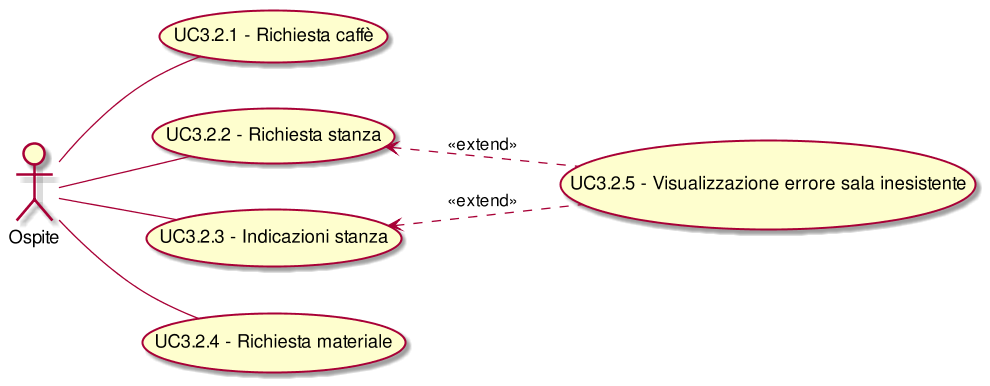
\includegraphics[width=\textwidth,height=\textheight,keepaspectratio]{images/UseCaseUC32.png}
\caption{UC3.2: Comunicazione necessità}
\end{figure}
\begin{longtable}{l|p{10cm}}
\rowcolor[gray]{0.8} \multicolumn{2}{c}{} \\
\rowcolor[gray]{0.8} \multicolumn{2}{c}{\textbf{UC3.2 - Comunicazione necessità}} \\
\rowcolor[gray]{0.8} \multicolumn{2}{c}{} \\
\hline
&\\
\textbf{Attori} & Assistente Virtuale, Ospite, Slack.\\[7pt]
\textbf{Descrizione} & Il sistema richiede all'ospite se ha particolari necessità per l'incontro.\\[7pt]
\textbf{Precondizione} & L'ospite si trova nella sezione adibita a comunicare particolari necessità riguardanti l'incontro.\\[7pt]
\textbf{Postcondizione} & Il sistema ha ricevuto le informazioni relative alle necessità dell'ospite e le ha comunicate alla persona desiderata tramite Slack.\\[7pt]
\textbf{Scenario principale} &\begin{enumerate}
\item  Il sistema può chiedere all'ospite se desidera un caffè;
\item  Il sistema può chiedere all'ospite se desidera informazioni relative alla locazione di una determinata stanza; 
\item  Il sistema può chiedere all'ospite se desidera del materiale particolare per l'incontro;
\item  Il sistema può chiedere all'ospite se desidera qualche altra necessità.
\end{enumerate}
\\[7pt]\hline
\end{longtable}

\subsubsection{UC3.2.1: Richiesta caffè}
\label{UC3.2.1}
\begin{longtable}{l|p{10cm}}
\rowcolor[gray]{0.8} \multicolumn{2}{c}{} \\
\rowcolor[gray]{0.8} \multicolumn{2}{c}{\textbf{UC3.2.1 - Richiesta caffè}} \\
\rowcolor[gray]{0.8} \multicolumn{2}{c}{} \\
\hline
&\\
\textbf{Attori} & Assistente Virtuale, Ospite, Slack.\\[7pt]
\textbf{Descrizione} & Il sistema può chiedere all'ospite se desidera un caffè prima dell'incontro.\\[7pt]
\textbf{Precondizione} & Il sistema ha chiesto all'ospite se desidera un caffè.\\[7pt]
\textbf{Postcondizione} & Il sistema ha ricevuto la risposta dell'ospite, comunicandola alla persona desiderata tramite Slack.\\[7pt]
\textbf{Scenario principale} &L'ospite può comunicare di volere o meno un caffè.\\[7pt]\hline
\end{longtable}

\subsubsection{UC3.2.2: Richiesta materiale}
\label{UC3.2.2}
\begin{longtable}{l|p{10cm}}
\rowcolor[gray]{0.8} \multicolumn{2}{c}{} \\
\rowcolor[gray]{0.8} \multicolumn{2}{c}{\textbf{UC3.2.2 - Richiesta materiale}} \\
\rowcolor[gray]{0.8} \multicolumn{2}{c}{} \\
\hline
&\\
\textbf{Attori} & Assistente Virtuale, Ospite, Slack.\\[7pt]
\textbf{Descrizione} & Il sistema può chiedere all'ospite se ha bisogno di materiale particolare per l'incontro.\\[7pt]
\textbf{Precondizione} & Il sistema ha chiesto all'ospite di quale materiale ha bisogno.\\[7pt]
\textbf{Postcondizione} & Il sistema ha ricevuto i dati relativi al materiale necessario all'ospite e li ha comunicati alla persona desiderata tramite Slack.\\[7pt]
\textbf{Scenario principale} &L'ospite comunica le sue necessità riguardanti il materiale per l'incontro.\\[7pt]\hline
\end{longtable}

\newpage\subsubsection{UC3.2.3: Indicazioni stanza}
\label{UC3.2.3}
\begin{figure}[h]
\centering
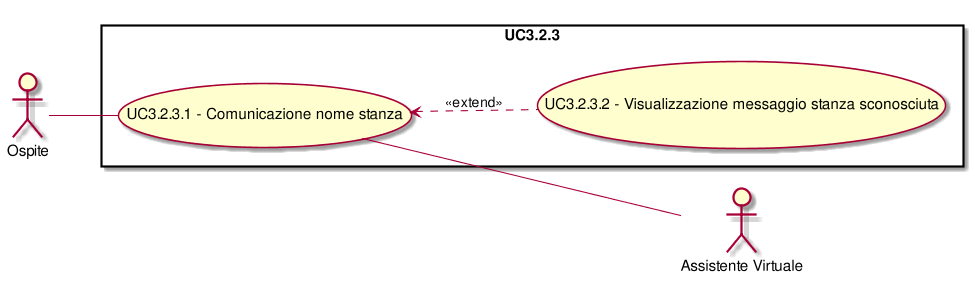
\includegraphics[width=\textwidth,height=\textheight,keepaspectratio]{images/UseCaseUC323.png}
\caption{UC3.2.3: Indicazioni stanza}
\end{figure}
\begin{longtable}{l|p{10cm}}
\rowcolor[gray]{0.8} \multicolumn{2}{c}{} \\
\rowcolor[gray]{0.8} \multicolumn{2}{c}{\textbf{UC3.2.3 - Indicazioni stanza}} \\
\rowcolor[gray]{0.8} \multicolumn{2}{c}{} \\
\hline
&\\
\textbf{Attori} & Assistente Virtuale, Ospite.\\[7pt]
\textbf{Descrizione} & Il sistema può ricevere la richiesta di informazioni relative alla locazione di una determinata stanza.\\[7pt]
\textbf{Precondizione} & L'ospite si trova nella sezione adibita a comunicare particolari necessità riguardanti l'incontro.\\[7pt]
\textbf{Postcondizione} & L'ospite ha chiesto le indicazioni.\\[7pt]
\textbf{Scenario principale} &\begin{enumerate}
\item  Il sistema chiede all'ospite il nome della stanza desiderata.
\end{enumerate}
\\[7pt]\hline
\end{longtable}

\subsubsection{UC3.2.3.1: Comunicazione nome stanza}
\label{UC3.2.3.1}
\begin{longtable}{l|p{10cm}}
\rowcolor[gray]{0.8} \multicolumn{2}{c}{} \\
\rowcolor[gray]{0.8} \multicolumn{2}{c}{\textbf{UC3.2.3.1 - Comunicazione nome stanza}} \\
\rowcolor[gray]{0.8} \multicolumn{2}{c}{} \\
\hline
&\\
\textbf{Attori} & Assistente Virtuale, Ospite.\\[7pt]
\textbf{Descrizione} & L'ospite può comunicare il nome della stanza desiderata al sistema, che mostrerà le indicazioni per raggiungerla.\\[7pt]
\textbf{Precondizione} & Il sistema ha richiesto all'ospite il nome della stanza desiderata.\\[7pt]
\textbf{Postcondizione} & Il sistema ha ricevuto il nome della stanza desiderata dall'ospite ed ha mostrato le indicazioni per raggiungerla.\\[7pt]
\textbf{Scenario principale} &Il sistema riceve il nome della stanza desiderata dall'ospite.\\[7pt]\hline
\end{longtable}

\newpage\subsubsection{UC3.2.3.2: Visualizzazione messaggio stanza sconosciuta}
\label{UC3.2.3.2}
\begin{longtable}{l|p{10cm}}
\rowcolor[gray]{0.8} \multicolumn{2}{c}{} \\
\rowcolor[gray]{0.8} \multicolumn{2}{c}{\textbf{UC3.2.3.2 - Visualizzazione messaggio stanza sconosciuta}} \\
\rowcolor[gray]{0.8} \multicolumn{2}{c}{} \\
\hline
&\\
\textbf{Attori} & Assistente Virtuale, Ospite.\\[7pt]
\textbf{Descrizione} & Il sistema può mostrare all'ospite un messaggio nel caso in cui il nome della stanza richiesta non sia riconosciuto.\\[7pt]
\textbf{Precondizione} & Il sistema ha ricevuto un nome di una stanza non presente nell'edificio.\\[7pt]
\textbf{Postcondizione} & Il sistema ha comunicato all'ospite che la stanza non è conosciuta.\\[7pt]
\textbf{Scenario principale} &Il sistema avverte l'ospite che la stanza richiesta non è conosciuta.\\[7pt]\hline
\end{longtable}

\subsubsection{UC3.2.4: Richiesta generica}
\label{UC3.2.4}
\begin{longtable}{l|p{10cm}}
\rowcolor[gray]{0.8} \multicolumn{2}{c}{} \\
\rowcolor[gray]{0.8} \multicolumn{2}{c}{\textbf{UC3.2.4 - Richiesta generica}} \\
\rowcolor[gray]{0.8} \multicolumn{2}{c}{} \\
\hline
&\\
\textbf{Attori} & Amministratore, Assistente Virtuale, Ospite, Slack.\\[7pt]
\textbf{Descrizione} & Il sistema può chiedere all'ospite altre necessità riguardanti l'incontro.\\[7pt]
\textbf{Precondizione} & Il sistema ha chiesto all'ospite se ha altre necessità per l'incontro.\\[7pt]
\textbf{Postcondizione} & Il sistema ha ricevuto i dati relativi alla necessità dell'ospite e li ha comunicati alla persona desiderata tramite Slack.\\[7pt]
\textbf{Scenario principale} &L'ospite comunica tutte le sue necessità ulteriori per l'incontro.\\[7pt]\hline
\end{longtable}

\newpage\subsubsection{UC3.3: Intrattenimento ospite}
\label{UC3.3}
\begin{figure}[h]
\centering
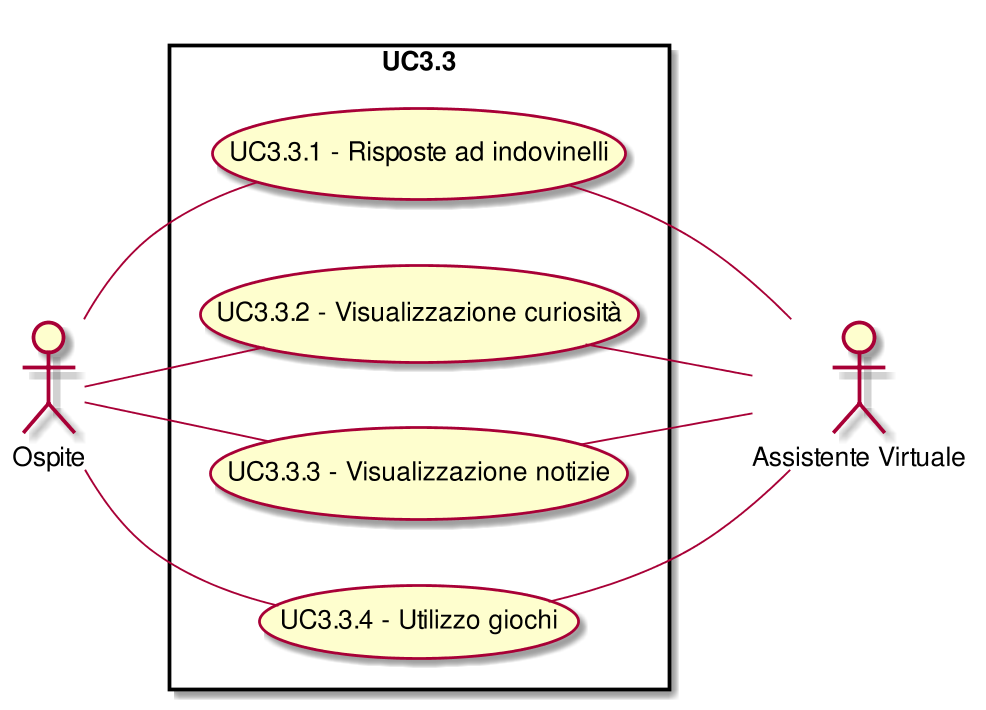
\includegraphics[width=\textwidth,height=\textheight,keepaspectratio]{images/UseCaseUC33.png}
\caption{UC3.3: Intrattenimento ospite}
\end{figure}
\begin{longtable}{l|p{10cm}}
\rowcolor[gray]{0.8} \multicolumn{2}{c}{} \\
\rowcolor[gray]{0.8} \multicolumn{2}{c}{\textbf{UC3.3 - Intrattenimento ospite}} \\
\rowcolor[gray]{0.8} \multicolumn{2}{c}{} \\
\hline
&\\
\textbf{Attori} & Assistente Virtuale, Ospite.\\[7pt]
\textbf{Descrizione} & L'ospite può scegliere tra alcuni tipi di intrattenimento forniti dal sistema, mentre attende l'arrivo della persona desiderata.\\[7pt]
\textbf{Precondizione} & L'ospite si trova nella sezione dedicata all'intrattenimento degli ospiti.\\[7pt]
\textbf{Postcondizione} & L'ospite ha usufruito degli intrattenimenti forniti dal sistema.\\[7pt]
\textbf{Scenario principale} &\begin{enumerate}
\item  L'ospite può essere intrattenuto con alcuni indovinelli ai quali deve rispondere;
\item  L'ospite può essere intrattenuto con alcune curiosità di varia natura;
\item  L'ospite può essere intrattenuto chiedendo di visualizzare alcune notizie di varia natura;
\item  L'ospite può essere intrattenuto con alcuni giochi che il sistema rende disponibili.
\end{enumerate}
\\[7pt]
\textbf{Scenari alternativi} & Dopo un certo lasso di tempo, l'ospite può sollecitare l'arrivo della persona desiderata.\\[7pt]\hline
\end{longtable}

\subsubsection{UC3.3.1: Indovinelli}
\label{UC3.3.1}
\begin{longtable}{l|p{10cm}}
\rowcolor[gray]{0.8} \multicolumn{2}{c}{} \\
\rowcolor[gray]{0.8} \multicolumn{2}{c}{\textbf{UC3.3.1 - Indovinelli}} \\
\rowcolor[gray]{0.8} \multicolumn{2}{c}{} \\
\hline
&\\
\textbf{Attori} & Assistente Virtuale, Ospite.\\[7pt]
\textbf{Descrizione} & L'ospite può rispondere ad alcuni indovinelli fatti dal sistema.\\[7pt]
\textbf{Precondizione} & L'ospite si trova nella sezione dedicata agli indovinelli.\\[7pt]
\textbf{Postcondizione} & L'ospite ha utilizzato le funzionalità degli indovinelli.\\[7pt]
\textbf{Scenario principale} &L'ospite interagisce con gli indovinelli forniti dal sistema.\\[7pt]\hline
\end{longtable}

\subsubsection{UC3.3.2: Visualizzazione curiosità}
\label{UC3.3.2}
\begin{longtable}{l|p{10cm}}
\rowcolor[gray]{0.8} \multicolumn{2}{c}{} \\
\rowcolor[gray]{0.8} \multicolumn{2}{c}{\textbf{UC3.3.2 - Visualizzazione curiosità}} \\
\rowcolor[gray]{0.8} \multicolumn{2}{c}{} \\
\hline
&\\
\textbf{Attori} & Assistente Virtuale, Ospite.\\[7pt]
\textbf{Descrizione} & L'ospite può essere intrattenuto dal sistema tramite la visualizzazione di curiosità di vario genere.\\[7pt]
\textbf{Precondizione} & L'ospite si trova nella sezione dedicata alla visualizzazione delle curiosità.\\[7pt]
\textbf{Postcondizione} & L'ospite ha visualizzato alcune curiosità.\\[7pt]
\textbf{Scenario principale} &L'ospite visualizza le curiosità fornite dal sistema.\\[7pt]\hline
\end{longtable}

\newpage\subsubsection{UC3.3.3: Notizie}
\label{UC3.3.3}
\begin{figure}[h]
\centering
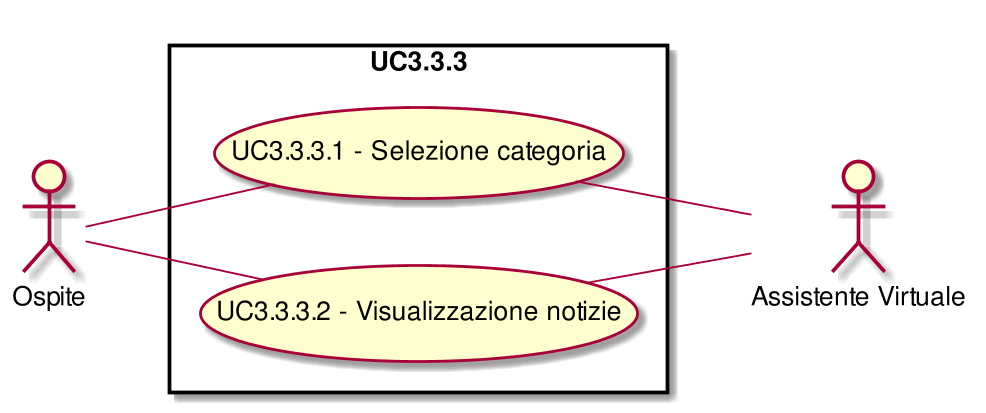
\includegraphics[width=\textwidth,height=\textheight,keepaspectratio]{images/UseCaseUC333.png}
\caption{UC3.3.3: Notizie}
\end{figure}
\begin{longtable}{l|p{10cm}}
\rowcolor[gray]{0.8} \multicolumn{2}{c}{} \\
\rowcolor[gray]{0.8} \multicolumn{2}{c}{\textbf{UC3.3.3 - Notizie}} \\
\rowcolor[gray]{0.8} \multicolumn{2}{c}{} \\
\hline
&\\
\textbf{Attori} & Assistente Virtuale, Ospite.\\[7pt]
\textbf{Descrizione} & L'ospite può essere intrattenuto chiedendo di visualizzare le ultime notizie riguardanti categorie di vario genere.\\[7pt]
\textbf{Precondizione} & L'ospite si trova nella sezione dedicata alla visualizzazione delle notizie.\\[7pt]
\textbf{Postcondizione} & L'ospite ha visualizzato le notizie da lui richieste.\\[7pt]
\textbf{Scenario principale} &L'ospite visualizza le notizie riguardanti la categoria richiesta.\\[7pt]\hline
\end{longtable}

\subsubsection{UC3.3.3.1: Selezione categoria}
\label{UC3.3.3.1}
\begin{longtable}{l|p{10cm}}
\rowcolor[gray]{0.8} \multicolumn{2}{c}{} \\
\rowcolor[gray]{0.8} \multicolumn{2}{c}{\textbf{UC3.3.3.1 - Selezione categoria}} \\
\rowcolor[gray]{0.8} \multicolumn{2}{c}{} \\
\hline
&\\
\textbf{Attori} & Assistente Virtuale, Ospite.\\[7pt]
\textbf{Descrizione} & Il sistema permette all'utente di selezionare la categoria di notizie da visualizzare.\\[7pt]
\textbf{Precondizione} & Il sistema ha richiesto all'ospite di selezionare la categoria di notizie.\\[7pt]
\textbf{Postcondizione} & L'ospite ha specificato la categoria di notizie alla quale è interessato.\\[7pt]
\textbf{Scenario principale} &L'ospite comunica al sistema la di categoria desiderata.\\[7pt]\hline
\end{longtable}

\subsubsection{UC3.3.3.2: Visualizzazione notizie}
\label{UC3.3.3.2}
\begin{longtable}{l|p{10cm}}
\rowcolor[gray]{0.8} \multicolumn{2}{c}{} \\
\rowcolor[gray]{0.8} \multicolumn{2}{c}{\textbf{UC3.3.3.2 - Visualizzazione notizie}} \\
\rowcolor[gray]{0.8} \multicolumn{2}{c}{} \\
\hline
&\\
\textbf{Attori} & Assistente Virtuale, Ospite.\\[7pt]
\textbf{Descrizione} & L'ospite può visualizzare le notizie fornite dal sistema.\\[7pt]
\textbf{Precondizione} & Il sistema ricevuto dall'ospite la categoria di notizie che desidera visualizzare.\\[7pt]
\textbf{Postcondizione} & Il sistema ha mostrato all'utente una notizia della categoria richiesta.\\[7pt]
\textbf{Scenario principale} &L'ospite visualizza la notizia fornita dal sistema.\\[7pt]\hline
\end{longtable}

\newpage\subsubsection{UC3.3.4: Utilizzo giochi}
\label{UC3.3.4}
\begin{figure}[h]
\centering
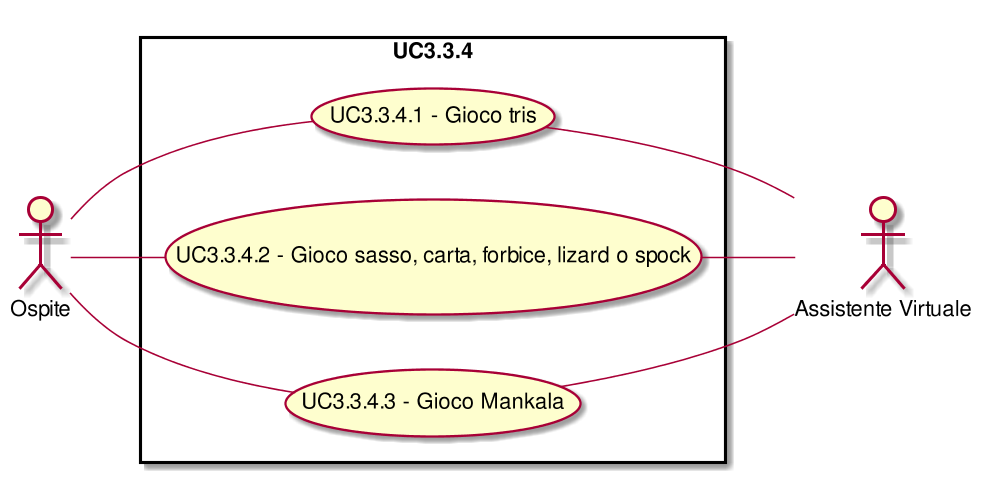
\includegraphics[width=\textwidth,height=\textheight,keepaspectratio]{images/UseCaseUC334.png}
\caption{UC3.3.4: Utilizzo giochi}
\end{figure}
\begin{longtable}{l|p{10cm}}
\rowcolor[gray]{0.8} \multicolumn{2}{c}{} \\
\rowcolor[gray]{0.8} \multicolumn{2}{c}{\textbf{UC3.3.4 - Utilizzo giochi}} \\
\rowcolor[gray]{0.8} \multicolumn{2}{c}{} \\
\hline
&\\
\textbf{Attori} & Assistente Virtuale, Ospite.\\[7pt]
\textbf{Descrizione} & L'ospite può essere intrattenuto tramite alcuni giochi forniti dal sistema.\\[7pt]
\textbf{Precondizione} & L'ospite si trova nella sezione dedicata ai giochi.\\[7pt]
\textbf{Postcondizione} & L'ospite ha interagito con i giochi forniti dal sistema.\\[7pt]
\textbf{Scenario principale} &L'ospite interagisce con i giochi forniti dal sistema.\\[7pt]\hline
\end{longtable}

\newpage\subsubsection{UC3.3.4.1: Gioco tris}
\label{UC3.3.4.1}
\begin{figure}[h]
\centering
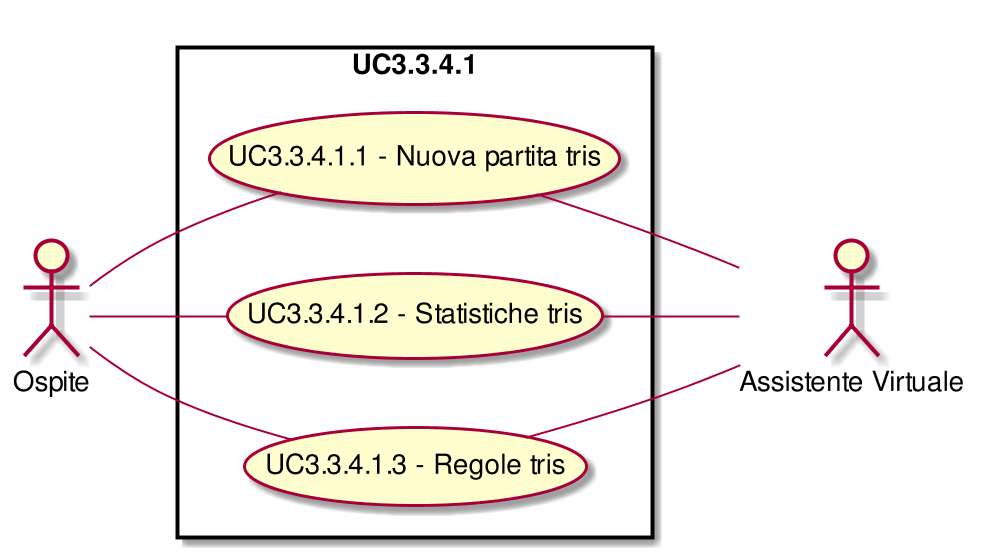
\includegraphics[width=\textwidth,height=\textheight,keepaspectratio]{images/UseCaseUC3341.png}
\caption{UC3.3.4.1: Gioco tris}
\end{figure}
\begin{longtable}{l|p{10cm}}
\rowcolor[gray]{0.8} \multicolumn{2}{c}{} \\
\rowcolor[gray]{0.8} \multicolumn{2}{c}{\textbf{UC3.3.4.1 - Gioco tris}} \\
\rowcolor[gray]{0.8} \multicolumn{2}{c}{} \\
\hline
&\\
\textbf{Attori} & Assistente Virtuale, Ospite.\\[7pt]
\textbf{Descrizione} & Il sistema può permettere all'ospite di giocare a tris.\\[7pt]
\textbf{Precondizione} & L'ospite si trova nella sezione dedicata al gioco del tris.\\[7pt]
\textbf{Postcondizione} & L'ospite ha terminato una partita a tris contro il sistema.\\[7pt]
\textbf{Scenario principale} &L'utente gioca una partita di tris contro il sistema.\\[7pt]\hline
\end{longtable}

\subsubsection{UC3.3.4.1.1: Nuova partita tris}
\label{UC3.3.4.1.1}
\begin{longtable}{l|p{10cm}}
\rowcolor[gray]{0.8} \multicolumn{2}{c}{} \\
\rowcolor[gray]{0.8} \multicolumn{2}{c}{\textbf{UC3.3.4.1.1 - Nuova partita tris}} \\
\rowcolor[gray]{0.8} \multicolumn{2}{c}{} \\
\hline
&\\
\textbf{Attori} & Assistente Virtuale, Ospite.\\[7pt]
\textbf{Descrizione} & Il sistema può permettere all'ospite di iniziare una nuova partita a tris.\\[7pt]
\textbf{Precondizione} & Il sistema ha avviato il gioco tris.
\\[7pt]
\textbf{Postcondizione} & Il sistema ha avviato una nuova partita di tris.
\\[7pt]
\textbf{Scenario principale} &L'ospite chiede al sistema di iniziare una nuova partita a tris.\\[7pt]\hline
\end{longtable}

\subsubsection{UC3.3.4.1.2: Statistiche tris}
\label{UC3.3.4.1.2}
\begin{longtable}{l|p{10cm}}
\rowcolor[gray]{0.8} \multicolumn{2}{c}{} \\
\rowcolor[gray]{0.8} \multicolumn{2}{c}{\textbf{UC3.3.4.1.2 - Statistiche tris}} \\
\rowcolor[gray]{0.8} \multicolumn{2}{c}{} \\
\hline
&\\
\textbf{Attori} & Assistente Virtuale, Ospite.\\[7pt]
\textbf{Descrizione} & Il sistema può offrire all'ospite la possibilità di visualizzare le statistiche delle partite.\\[7pt]
\textbf{Precondizione} & Il sistema ha avviato il gioco tris.\\[7pt]
\textbf{Postcondizione} & Il sistema ha mostrato le statistiche delle partite all'ospite.\\[7pt]
\textbf{Scenario principale} &L'ospite ha richiesto di visualizzare le statistiche delle partite.\\[7pt]\hline
\end{longtable}

\subsubsection{UC3.3.4.1.3: Regole tris}
\label{UC3.3.4.1.3}
\begin{longtable}{l|p{10cm}}
\rowcolor[gray]{0.8} \multicolumn{2}{c}{} \\
\rowcolor[gray]{0.8} \multicolumn{2}{c}{\textbf{UC3.3.4.1.3 - Regole tris}} \\
\rowcolor[gray]{0.8} \multicolumn{2}{c}{} \\
\hline
&\\
\textbf{Attori} & Assistente Virtuale, Ospite.\\[7pt]
\textbf{Descrizione} & Il sistema può permettere all'ospite di visualizzare le regole del gioco tris.\\[7pt]
\textbf{Precondizione} & Il sistema ha avviato il gioco tris.\\[7pt]
\textbf{Postcondizione} & Il sistema ha mostrato all'ospite le regole del gioco tris.\\[7pt]
\textbf{Scenario principale} &L'ospite chiede le regole del gioco tris.\\[7pt]\hline
\end{longtable}

\newpage\subsubsection{UC3.3.4.2: Gioco sasso, carta, forbice, lizard o spock}
\label{UC3.3.4.2}
\begin{figure}[h]
\centering
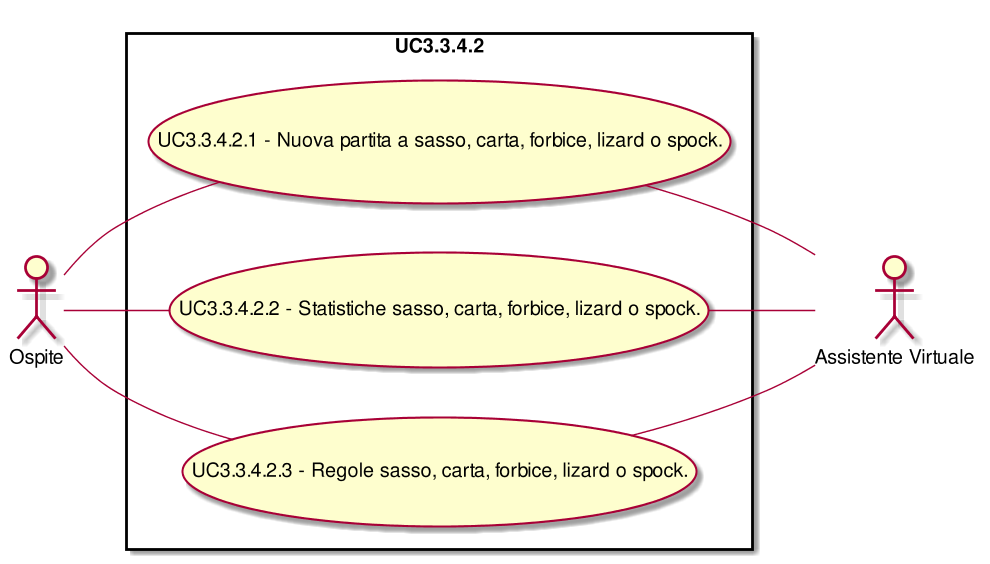
\includegraphics[width=\textwidth,height=\textheight,keepaspectratio]{images/UseCaseUC3342.png}
\caption{UC3.3.4.2: Gioco sasso, carta, forbice, lizard o spock}
\end{figure}
\begin{longtable}{l|p{10cm}}
\rowcolor[gray]{0.8} \multicolumn{2}{c}{} \\
\rowcolor[gray]{0.8} \multicolumn{2}{c}{\textbf{UC3.3.4.2 - Gioco sasso, carta, forbice, lizard o spock}} \\
\rowcolor[gray]{0.8} \multicolumn{2}{c}{} \\
\hline
&\\
\textbf{Attori} & Assistente Virtuale, Ospite.\\[7pt]
\textbf{Descrizione} & Il sistema può permettere all'ospite di giocare a  sasso, carta, forbice, lizard o spock.\\[7pt]
\textbf{Precondizione} & L'ospite si trova nella sezione dedicata al gioco sasso, carta, forbice, lizard o spock.\\[7pt]
\textbf{Postcondizione} & L'ospite ha terminato una partita a sasso, carta, forbice, lizard o spock contro il sistema.\\[7pt]
\textbf{Scenario principale} &L'utente gioca una partita a sasso, carta, forbice, lizard o spock contro il sistema.\\[7pt]\hline
\end{longtable}

\subsubsection{UC3.3.4.2.1: Nuova partita a sasso, carta, forbice, lizard o spock.}
\label{UC3.3.4.2.1}
\begin{longtable}{l|p{10cm}}
\rowcolor[gray]{0.8} \multicolumn{2}{c}{} \\
\rowcolor[gray]{0.8} \multicolumn{2}{c}{\textbf{UC3.3.4.2.1 - Nuova partita a sasso, carta, forbice, lizard o spock.}} \\
\rowcolor[gray]{0.8} \multicolumn{2}{c}{} \\
\hline
&\\
\textbf{Attori} & Assistente Virtuale, Ospite.\\[7pt]
\textbf{Descrizione} & Il sistema può permettere all'ospite di iniziare una nuova partita a sasso, carta, forbice, lizard o spock.\\[7pt]
\textbf{Precondizione} & Il sistema ha avviato il gioco sasso, carta, forbice, lizard o spock.\\[7pt]
\textbf{Postcondizione} & Il sistema ha avviato una nuova partita a sasso, carta, forbice, lizard o spock.\\[7pt]
\textbf{Scenario principale} &L'ospite chiede al sistema di iniziare una nuova partita a sasso, carta, forbice, lizard o spock.\\[7pt]\hline
\end{longtable}

\subsubsection{UC3.3.4.2.2: Statistiche sasso, carta, forbice, lizard o spock.}
\label{UC3.3.4.2.2}
\begin{longtable}{l|p{10cm}}
\rowcolor[gray]{0.8} \multicolumn{2}{c}{} \\
\rowcolor[gray]{0.8} \multicolumn{2}{c}{\textbf{UC3.3.4.2.2 - Statistiche sasso, carta, forbice, lizard o spock.}} \\
\rowcolor[gray]{0.8} \multicolumn{2}{c}{} \\
\hline
&\\
\textbf{Attori} & Assistente Virtuale, Ospite.\\[7pt]
\textbf{Descrizione} & Il sistema può offrire all'ospite la possibilità di visualizzare le statistiche delle partite.\\[7pt]
\textbf{Precondizione} & Il sistema ha avviato il gioco sasso, carta, forbice, lizard o spock.\\[7pt]
\textbf{Postcondizione} & Il sistema ha mostrato le statistiche delle partite all'ospite.\\[7pt]
\textbf{Scenario principale} &L'ospite ha richiesto di visualizzare le statistiche delle partite.\\[7pt]\hline
\end{longtable}

\subsubsection{UC3.3.4.2.3: Regole sasso, carta, forbice, lizard o spock.}
\label{UC3.3.4.2.3}
\begin{longtable}{l|p{10cm}}
\rowcolor[gray]{0.8} \multicolumn{2}{c}{} \\
\rowcolor[gray]{0.8} \multicolumn{2}{c}{\textbf{UC3.3.4.2.3 - Regole sasso, carta, forbice, lizard o spock.}} \\
\rowcolor[gray]{0.8} \multicolumn{2}{c}{} \\
\hline
&\\
\textbf{Attori} & Assistente Virtuale, Ospite.\\[7pt]
\textbf{Descrizione} & Il sistema può permettere all'ospite di visualizzare le regole del gioco sasso, carta, forbice, lizard o spock.\\[7pt]
\textbf{Precondizione} & Il sistema ha avviato il gioco sasso, carta, forbice, lizard o spock.\\[7pt]
\textbf{Postcondizione} & Il sistema ha mostrato all'ospite le regole del gioco sasso, carta, forbice, lizard o spock.\\[7pt]
\textbf{Scenario principale} &L'ospite chiede le regole del gioco sasso, carta, forbice, lizard o spock.\\[7pt]\hline
\end{longtable}

\newpage\subsubsection{UC3.3.4.3: Gioco Mankala}
\label{UC3.3.4.3}
\begin{figure}[h]
\centering
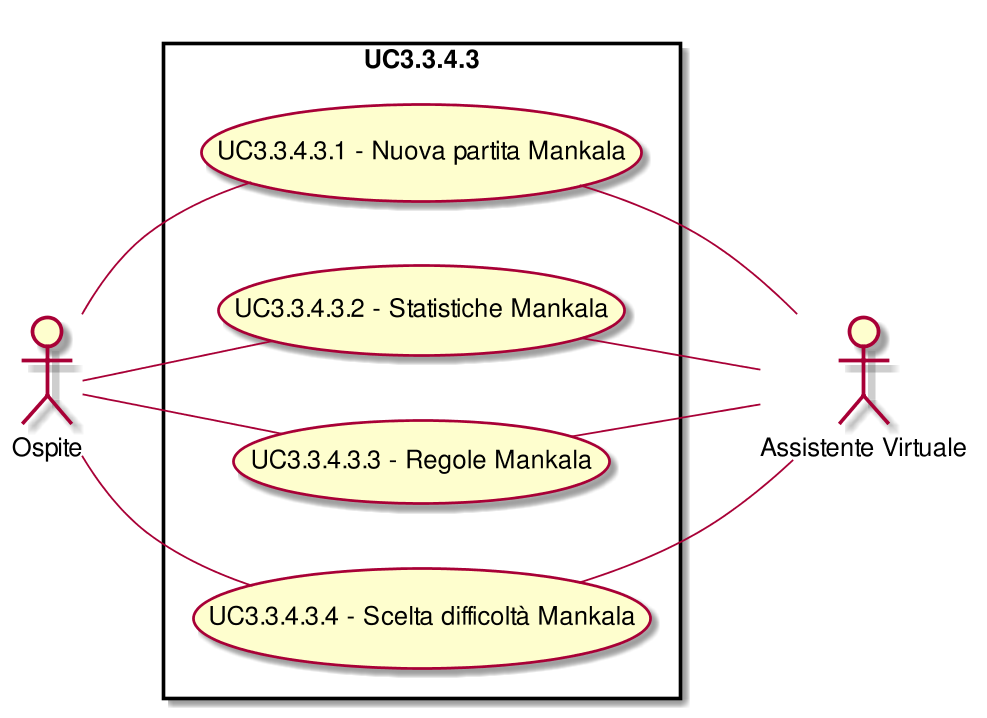
\includegraphics[width=\textwidth,height=\textheight,keepaspectratio]{images/UseCaseUC3343.png}
\caption{UC3.3.4.3: Gioco Mankala}
\end{figure}
\begin{longtable}{l|p{10cm}}
\rowcolor[gray]{0.8} \multicolumn{2}{c}{} \\
\rowcolor[gray]{0.8} \multicolumn{2}{c}{\textbf{UC3.3.4.3 - Gioco Mankala}} \\
\rowcolor[gray]{0.8} \multicolumn{2}{c}{} \\
\hline
&\\
\textbf{Attori} & Assistente Virtuale, Ospite.\\[7pt]
\textbf{Descrizione} & Il sistema può permettere all'ospite di giocare a Mankala.\\[7pt]
\textbf{Precondizione} & L'ospite si trova nella sezione dedicata al gioco Mankala.\\[7pt]
\textbf{Postcondizione} & L'ospite ha terminato una partita a Mankala contro il sistema.\\[7pt]
\textbf{Scenario principale} &L'ospite gioca una partita a Mankala contro il sistema.\\[7pt]\hline
\end{longtable}

\subsubsection{UC3.3.4.3.1: Nuova partita Mankala}
\label{UC3.3.4.3.1}
\begin{longtable}{l|p{10cm}}
\rowcolor[gray]{0.8} \multicolumn{2}{c}{} \\
\rowcolor[gray]{0.8} \multicolumn{2}{c}{\textbf{UC3.3.4.3.1 - Nuova partita Mankala}} \\
\rowcolor[gray]{0.8} \multicolumn{2}{c}{} \\
\hline
&\\
\textbf{Attori} & Assistente Virtuale, Ospite.\\[7pt]
\textbf{Descrizione} & Il sistema può permettere all'ospite di iniziare una nuova partita a Mankala.\\[7pt]
\textbf{Precondizione} & Il sistema ha avviato il gioco Mankala.\\[7pt]
\textbf{Postcondizione} & Il sistema ha avviato una nuova partita di Mankala.\\[7pt]
\textbf{Scenario principale} &L'ospite chiede al sistema di iniziare una nuova partita a Mankala.\\[7pt]\hline
\end{longtable}

\subsubsection{UC3.3.4.3.2: Statistiche Mankala}
\label{UC3.3.4.3.2}
\begin{longtable}{l|p{10cm}}
\rowcolor[gray]{0.8} \multicolumn{2}{c}{} \\
\rowcolor[gray]{0.8} \multicolumn{2}{c}{\textbf{UC3.3.4.3.2 - Statistiche Mankala}} \\
\rowcolor[gray]{0.8} \multicolumn{2}{c}{} \\
\hline
&\\
\textbf{Attori} & Assistente Virtuale, Ospite.\\[7pt]
\textbf{Descrizione} & Il sistema può offrire all'ospite la possibilità di visualizzare le statistiche delle partite.\\[7pt]
\textbf{Precondizione} & Il sistema ha avviato il gioco Mankala.\\[7pt]
\textbf{Postcondizione} & Il sistema ha mostrato le statistiche delle partite all'ospite.\\[7pt]
\textbf{Scenario principale} &L'ospite ha richiesto di visualizzare le statistiche delle partite.\\[7pt]\hline
\end{longtable}

\subsubsection{UC3.3.4.3.3: Regole Mankala}
\label{UC3.3.4.3.3}
\begin{longtable}{l|p{10cm}}
\rowcolor[gray]{0.8} \multicolumn{2}{c}{} \\
\rowcolor[gray]{0.8} \multicolumn{2}{c}{\textbf{UC3.3.4.3.3 - Regole Mankala}} \\
\rowcolor[gray]{0.8} \multicolumn{2}{c}{} \\
\hline
&\\
\textbf{Attori} & Assistente Virtuale, Ospite.\\[7pt]
\textbf{Descrizione} & Il sistema può permettere all'ospite di visualizzare le regole del gioco Mankala.\\[7pt]
\textbf{Precondizione} & Il sistema ha avviato il gioco Mankala.\\[7pt]
\textbf{Postcondizione} & Il sistema ha mostrato all'ospite le regole del gioco Mankala.\\[7pt]
\textbf{Scenario principale} &L'ospite chiede le regole del gioco Mankala.\\[7pt]\hline
\end{longtable}

\subsubsection{UC3.3.4.3.4: Scelta difficoltà Mankala}
\label{UC3.3.4.3.4}
\begin{longtable}{l|p{10cm}}
\rowcolor[gray]{0.8} \multicolumn{2}{c}{} \\
\rowcolor[gray]{0.8} \multicolumn{2}{c}{\textbf{UC3.3.4.3.4 - Scelta difficoltà Mankala}} \\
\rowcolor[gray]{0.8} \multicolumn{2}{c}{} \\
\hline
&\\
\textbf{Attori} & Assistente Virtuale, Ospite.\\[7pt]
\textbf{Descrizione} & Il sistema può offrire all'ospite la possibilità di scegliere la difficoltà delle partite di Mankala.\\[7pt]
\textbf{Precondizione} & Il sistema ha avviato il gioco Mankala.\\[7pt]
\textbf{Postcondizione} & Il sistema ha impostato la difficoltà delle partite di Mankala.\\[7pt]
\textbf{Scenario principale} &L'ospite ha richiesto di impostare la difficoltà del Mankala.\\[7pt]\hline
\end{longtable}

\newpage\subsection{UC4: Accesso funzionalità super amministratore}
\label{UC4}
\begin{figure}[h]
\centering
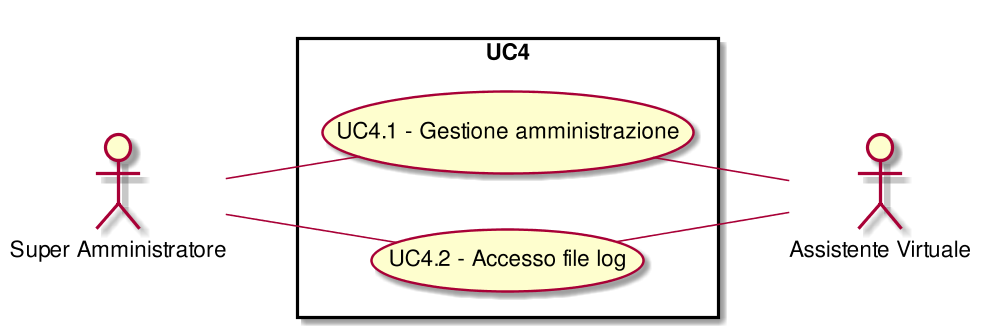
\includegraphics[width=\textwidth,height=\textheight,keepaspectratio]{images/UseCaseUC4.png}
\caption{UC4: Accesso funzionalità super amministratore}
\end{figure}
\begin{longtable}{l|p{10cm}}
\rowcolor[gray]{0.8} \multicolumn{2}{c}{} \\
\rowcolor[gray]{0.8} \multicolumn{2}{c}{\textbf{UC4 - Accesso funzionalità super amministratore}} \\
\rowcolor[gray]{0.8} \multicolumn{2}{c}{} \\
\hline
&\\
\textbf{Attori} & Super Amministratore.\\[7pt]
\textbf{Descrizione} & Il super amministratore può gestire gli amministratori ed accedere ai file \gl{log}.\\[7pt]
\textbf{Precondizione} & Il super amministratore si trova nella sezione adibita alla gestione.\\[7pt]
\textbf{Postcondizione} & Il super amministratore ha usufruito delle funzionalità di gestione.\\[7pt]
\textbf{Scenario principale} &\begin{enumerate}
\item  Il super amministratore può gestire gli amministratori del sistema; 
\item  Il super amministratore può accedere ai file log.
\end{enumerate}
\\[7pt]\hline
\end{longtable}

\newpage\subsubsection{UC4.1: Gestione amministrazione}
\label{UC4.1}
\begin{figure}[h]
\centering
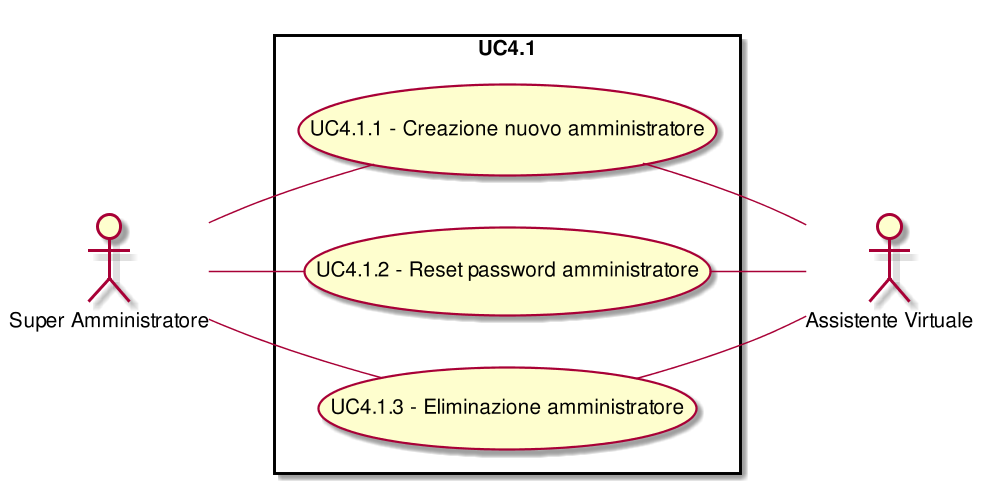
\includegraphics[width=\textwidth,height=\textheight,keepaspectratio]{images/UseCaseUC41.png}
\caption{UC4.1: Gestione amministrazione}
\end{figure}
\begin{longtable}{l|p{10cm}}
\rowcolor[gray]{0.8} \multicolumn{2}{c}{} \\
\rowcolor[gray]{0.8} \multicolumn{2}{c}{\textbf{UC4.1 - Gestione amministrazione}} \\
\rowcolor[gray]{0.8} \multicolumn{2}{c}{} \\
\hline
&\\
\textbf{Attori} & Assistente Virtuale, Super Amministratore.\\[7pt]
\textbf{Descrizione} & Il super amministratore può gestire gli amministratori del sistema.\\[7pt]
\textbf{Precondizione} & Il super amministratore si trova nella sezione per gestire gli amministratori.\\[7pt]
\textbf{Postcondizione} & Il super amministratore ha usufruito delle funzionalità per gestire gli amministratori.\\[7pt]
\textbf{Scenario principale} &\begin{enumerate}
\item  Il super amministratore può creare un nuovo amministratore;
\item  Il super amministratore può resettare la password degli amministratori;
\item  Il super amministratore può revocare i privilegi degli amministratori.
\end{enumerate}
\\[7pt]\hline
\end{longtable}

\newpage\subsubsection{UC4.1.1: Creazione nuovo amministratore}
\label{UC4.1.1}
\begin{figure}[h]
\centering
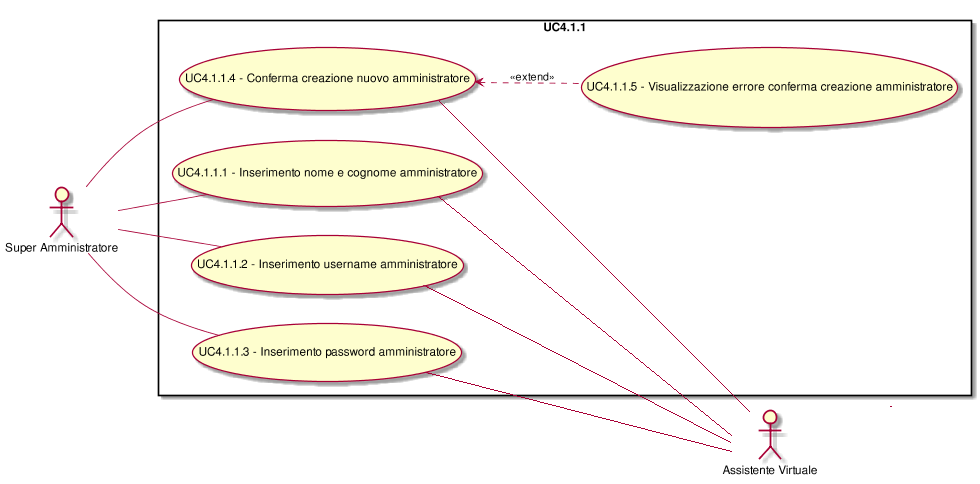
\includegraphics[width=\textwidth,height=\textheight,keepaspectratio]{images/UseCaseUC411.png}
\caption{UC4.1.1: Creazione nuovo amministratore}
\end{figure}
\begin{longtable}{l|p{10cm}}
\rowcolor[gray]{0.8} \multicolumn{2}{c}{} \\
\rowcolor[gray]{0.8} \multicolumn{2}{c}{\textbf{UC4.1.1 - Creazione nuovo amministratore}} \\
\rowcolor[gray]{0.8} \multicolumn{2}{c}{} \\
\hline
&\\
\textbf{Attori} & Assistente Virtuale, Super Amministratore.\\[7pt]
\textbf{Descrizione} & Il super amministratore può creare un nuovo amministratore.\\[7pt]
\textbf{Precondizione} & Il super amministratore si trova nella sezione per creare un nuovo amministratore.\\[7pt]
\textbf{Postcondizione} & Il super amministratore ha creato un nuovo amministratore.\\[7pt]
\textbf{Scenario principale} &\begin{enumerate}
\item  Il super amministratore può inserire nome e cognome dell'amministratore;
\item  Il super amministratore può inserire la password dell'amministratore;
\item  Il super amministratore può confermare il nuovo amministratore.
\end{enumerate}
\\[7pt]
\textbf{Scenari alternativi} & Il super amministratore visualizza un messaggio d'errore relativo alla conferma della creazione dell'amministratore.\\[7pt]\hline
\end{longtable}

\newpage\subsubsection{UC4.1.1.1: Inserimento nome e cognome amministratore}
\label{UC4.1.1.1}
\begin{longtable}{l|p{10cm}}
\rowcolor[gray]{0.8} \multicolumn{2}{c}{} \\
\rowcolor[gray]{0.8} \multicolumn{2}{c}{\textbf{UC4.1.1.1 - Inserimento nome e cognome amministratore}} \\
\rowcolor[gray]{0.8} \multicolumn{2}{c}{} \\
\hline
&\\
\textbf{Attori} & Assistente Virtuale, Super Amministratore.\\[7pt]
\textbf{Descrizione} & Il super amministratore può inserire nome e cognome del nuovo amministratore.\\[7pt]
\textbf{Precondizione} & Il super amministratore si trova nella sezione per creare un nuovo amministratore. \\[7pt]
\textbf{Postcondizione} & Il super amministratore ha inserito nome e cognome del nuovo amministratore.\\[7pt]
\textbf{Scenario principale} &Il super amministratore inserisce nome e cognome di un nuovo amministratore.\\[7pt]\hline
\end{longtable}

\subsubsection{UC4.1.1.2: Inserimento username amministratore}
\label{UC4.1.1.2}
\begin{longtable}{l|p{10cm}}
\rowcolor[gray]{0.8} \multicolumn{2}{c}{} \\
\rowcolor[gray]{0.8} \multicolumn{2}{c}{\textbf{UC4.1.1.2 - Inserimento username amministratore}} \\
\rowcolor[gray]{0.8} \multicolumn{2}{c}{} \\
\hline
&\\
\textbf{Attori} & Assistente Virtuale, Super Amministratore.\\[7pt]
\textbf{Descrizione} & Il super amministratore può inserire lo username di un nuovo amministratore.\\[7pt]
\textbf{Precondizione} & Il super amministratore si trova nella sezione per la creazione di un nuovo amministratore.\\[7pt]
\textbf{Postcondizione} & Il sistema ha ricevuto lo username di un nuovo amministratore.\\[7pt]
\textbf{Scenario principale} &Il super amministratore fornisce al sistema lo username di un nuovo amministratore.\\[7pt]\hline
\end{longtable}

\subsubsection{UC4.1.1.3: Inserimento password amministratore}
\label{UC4.1.1.3}
\begin{longtable}{l|p{10cm}}
\rowcolor[gray]{0.8} \multicolumn{2}{c}{} \\
\rowcolor[gray]{0.8} \multicolumn{2}{c}{\textbf{UC4.1.1.3 - Inserimento password amministratore}} \\
\rowcolor[gray]{0.8} \multicolumn{2}{c}{} \\
\hline
&\\
\textbf{Attori} & Assistente Virtuale, Super Amministratore.\\[7pt]
\textbf{Descrizione} & Il super amministratore può inserire la password di un nuovo amministratore.\\[7pt]
\textbf{Precondizione} & Il super amministratore si trova nella sezione per creare un nuovo amministratore. \\[7pt]
\textbf{Postcondizione} & Il super amministratore ha inserito la password del nuovo amministratore.\\[7pt]
\textbf{Scenario principale} &Il super amministratore inserisce la password per il nuovo amministratore.\\[7pt]\hline
\end{longtable}

\subsubsection{UC4.1.1.4: Conferma creazione nuovo amministratore}
\label{UC4.1.1.4}
\begin{longtable}{l|p{10cm}}
\rowcolor[gray]{0.8} \multicolumn{2}{c}{} \\
\rowcolor[gray]{0.8} \multicolumn{2}{c}{\textbf{UC4.1.1.4 - Conferma creazione nuovo amministratore}} \\
\rowcolor[gray]{0.8} \multicolumn{2}{c}{} \\
\hline
&\\
\textbf{Attori} & Assistente Virtuale, Super Amministratore.\\[7pt]
\textbf{Descrizione} & Il super amministratore può confermare i dati inseriti per la creazione di un nuovo amministratore.\\[7pt]
\textbf{Precondizione} & Il super amministratore si trova nella sezione per creare un nuovo amministratore. \\[7pt]
\textbf{Postcondizione} & Il super amministratore ha confermato la creazione del nuovo amministratore.\\[7pt]
\textbf{Scenario principale} &Il super amministratore conferma la creazione di un nuovo amministratore.\\[7pt]
\textbf{Scenari alternativi} & Il super amministratore non conferma di voler creare il nuovo amministratore. Il super amministratore viene rimandato alla pagina dedicata alla gestione degli amministratori.\\[7pt]\hline
\end{longtable}

\subsubsection{UC4.1.1.5: Visualizzazione errore conferma creazione amministratore}
\label{UC4.1.1.5}
\begin{longtable}{l|p{10cm}}
\rowcolor[gray]{0.8} \multicolumn{2}{c}{} \\
\rowcolor[gray]{0.8} \multicolumn{2}{c}{\textbf{UC4.1.1.5 - Visualizzazione errore conferma creazione amministratore}} \\
\rowcolor[gray]{0.8} \multicolumn{2}{c}{} \\
\hline
&\\
\textbf{Attori} & Assistente Virtuale, Super Amministratore.\\[7pt]
\textbf{Descrizione} & Il super amministratore può visualizzare un messaggio d'errore se ha comunicato dei dati non validi per la creazione di un nuovo amministratore.
I dati non validi sono: username già esistente.\\[7pt]
\textbf{Precondizione} & Il sistema ha ricevuto dati non validi.\\[7pt]
\textbf{Postcondizione} & Il sistema mostra un messaggio d'errore.\\[7pt]
\textbf{Scenario principale} &Il super amministratore visualizza un messaggio d'errore.\\[7pt]\hline
\end{longtable}

\newpage\subsubsection{UC4.1.2: Reset password amministratore}
\label{UC4.1.2}
\begin{figure}[h]
\centering
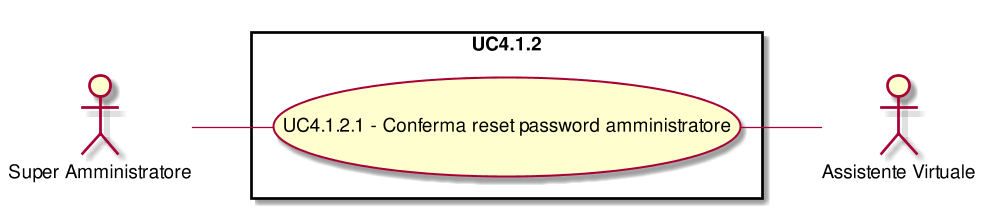
\includegraphics[width=\textwidth,height=\textheight,keepaspectratio]{images/UseCaseUC412.png}
\caption{UC4.1.2: Reset password amministratore}
\end{figure}
\begin{longtable}{l|p{10cm}}
\rowcolor[gray]{0.8} \multicolumn{2}{c}{} \\
\rowcolor[gray]{0.8} \multicolumn{2}{c}{\textbf{UC4.1.2 - Reset password amministratore}} \\
\rowcolor[gray]{0.8} \multicolumn{2}{c}{} \\
\hline
&\\
\textbf{Attori} & Assistente Virtuale, Super Amministratore.\\[7pt]
\textbf{Descrizione} & Il super amministratore può resettare la password dell'amministratore.\\[7pt]
\textbf{Precondizione} & Il super amministratore si trova nella sezione per resettare la password di un amministratore.\\[7pt]
\textbf{Postcondizione} & Il super amministratore ha resettato la password dell'amministratore.\\[7pt]
\textbf{Scenario principale} &\begin{enumerate}
\item  Il super amministratore può inserire la nuova password dell'amministratore;
\item  il super amministratore può confermare la nuova password dell'amministratore;
\item  il super amministratore può confermare il reset della password.
\end{enumerate}
\\[7pt]
\textbf{Scenari alternativi} & Il super amministratore visualizza un messaggio d'errore relativo al reset della password dell'amministratore.\\[7pt]\hline
\end{longtable}

\subsubsection{UC4.1.2.1: Conferma reset password amministratore}
\label{UC4.1.2.1}
\begin{longtable}{l|p{10cm}}
\rowcolor[gray]{0.8} \multicolumn{2}{c}{} \\
\rowcolor[gray]{0.8} \multicolumn{2}{c}{\textbf{UC4.1.2.1 - Conferma reset password amministratore}} \\
\rowcolor[gray]{0.8} \multicolumn{2}{c}{} \\
\hline
&\\
\textbf{Attori} & Assistente Virtuale, Super Amministratore.\\[7pt]
\textbf{Descrizione} & Il super amministratore può confermare il reset della password.\\[7pt]
\textbf{Precondizione} & Il super amministratore si trova nella sezione per confermare il reset della password dell'amministratore.\\[7pt]
\textbf{Postcondizione} & Il super amministratore ha confermato il reset della password dell'amministratore.\\[7pt]
\textbf{Scenario principale} &Il super amministratore conferma il reset della password dell'amministratore.\\[7pt]
\textbf{Scenari alternativi} & Il super amministratore non conferma di voler resettare la password dell'amministratore. Il super amministratore viene rimandato alla pagina dedicata alla gestione degli amministratori.\\[7pt]\hline
\end{longtable}

\newpage\subsubsection{UC4.1.3: Eliminazione amministratore}
\label{UC4.1.3}
\begin{figure}[h]
\centering
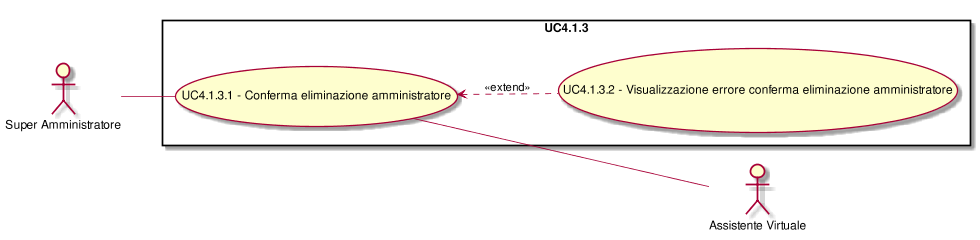
\includegraphics[width=\textwidth,height=\textheight,keepaspectratio]{images/UseCaseUC413.png}
\caption{UC4.1.3: Eliminazione amministratore}
\end{figure}
\begin{longtable}{l|p{10cm}}
\rowcolor[gray]{0.8} \multicolumn{2}{c}{} \\
\rowcolor[gray]{0.8} \multicolumn{2}{c}{\textbf{UC4.1.3 - Eliminazione amministratore}} \\
\rowcolor[gray]{0.8} \multicolumn{2}{c}{} \\
\hline
&\\
\textbf{Attori} & Assistente Virtuale, Super Amministratore.\\[7pt]
\textbf{Descrizione} & Il super amministratore può rimuovere un amministratore dal sistema\\[7pt]
\textbf{Precondizione} & Il super amministratore si trova nella sezione per l'eliminazione di un amministratore.\\[7pt]
\textbf{Postcondizione} & Il super amministratore ha eliminato un amministratore dal sistema.\\[7pt]
\textbf{Scenario principale} &\begin{enumerate}
\item  Il super amministratore può eliminare un amministratore;
\item  il super amministratore può confermare l'eliminazione dell'amministratore.
\end{enumerate}
\\[7pt]
\textbf{Scenari alternativi} & Il super amministratore visualizza un messaggio d'errore relativo alla revoca dei privilegi dell'amministratore.\\[7pt]\hline
\end{longtable}

\subsubsection{UC4.1.3.1: Conferma eliminazione amministratore}
\label{UC4.1.3.1}
\begin{longtable}{l|p{10cm}}
\rowcolor[gray]{0.8} \multicolumn{2}{c}{} \\
\rowcolor[gray]{0.8} \multicolumn{2}{c}{\textbf{UC4.1.3.1 - Conferma eliminazione amministratore}} \\
\rowcolor[gray]{0.8} \multicolumn{2}{c}{} \\
\hline
&\\
\textbf{Attori} & Assistente Virtuale, Super Amministratore.\\[7pt]
\textbf{Descrizione} & Il super amministratore può confermare l'eliminazione di un amministratore.\\[7pt]
\textbf{Precondizione} & Il super amministratore ha comunicato l'amministratore che vuole eliminare.\\[7pt]
\textbf{Postcondizione} & Il super amministratore ha eliminato un amministratore.\\[7pt]
\textbf{Scenario principale} &Il super amministratore conferma di volere eliminare un amministratore.\\[7pt]
\textbf{Scenari alternativi} & Il super amministratore non conferma di voler eliminare l'amministratore. Il super amministratore viene rimandato alla pagina dedicata alla gestione degli amministratori.\\[7pt]\hline
\end{longtable}

\subsubsection{UC4.1.3.2: Visualizzazione errore conferma eliminazione amministratore}
\label{UC4.1.3.2}
\begin{longtable}{l|p{10cm}}
\rowcolor[gray]{0.8} \multicolumn{2}{c}{} \\
\rowcolor[gray]{0.8} \multicolumn{2}{c}{\textbf{UC4.1.3.2 - Visualizzazione errore conferma eliminazione amministratore}} \\
\rowcolor[gray]{0.8} \multicolumn{2}{c}{} \\
\hline
&\\
\textbf{Attori} & Assistente Virtuale, Super Amministratore.\\[7pt]
\textbf{Descrizione} & L'amministratore può visualizzare un messaggio d'errore se ha comunicato dei dati non validi per l'eliminazione di un amministratore.
I dati non validi sono: username amministratore inesistente.\\[7pt]
\textbf{Precondizione} & Il sistema ha ricevuto dati non validi.\\[7pt]
\textbf{Postcondizione} & Il sistema mostra un messaggio d'errore.\\[7pt]
\textbf{Scenario principale} &Il super amministratore visualizza un messaggio d'errore.\\[7pt]\hline
\end{longtable}

\subsubsection{UC4.2: Accesso file log}
\label{UC4.2}
\begin{longtable}{l|p{10cm}}
\rowcolor[gray]{0.8} \multicolumn{2}{c}{} \\
\rowcolor[gray]{0.8} \multicolumn{2}{c}{\textbf{UC4.2 - Accesso file log}} \\
\rowcolor[gray]{0.8} \multicolumn{2}{c}{} \\
\hline
&\\
\textbf{Attori} & Assistente Virtuale, Super Amministratore.\\[7pt]
\textbf{Descrizione} & Il super amministratore può accedere ai file log.\\[7pt]
\textbf{Precondizione} & Il super amministratore si trova nella sezione adibita alla visualizzazione dei file log.\\[7pt]
\textbf{Postcondizione} & Il super amministratore ha fatto accesso ai file log.\\[7pt]
\textbf{Scenario principale} &Il super amministratore accede e visualizza i file log.\\[7pt]\hline
\end{longtable}

\subsection{UC5: Comunicazione non comprensibile}
\label{UC5}
\begin{longtable}{l|p{10cm}}
\rowcolor[gray]{0.8} \multicolumn{2}{c}{} \\
\rowcolor[gray]{0.8} \multicolumn{2}{c}{\textbf{UC5 - Comunicazione non comprensibile}} \\
\rowcolor[gray]{0.8} \multicolumn{2}{c}{} \\
\hline
&\\
\textbf{Attori} & Assistente Virtuale.\\[7pt]
\textbf{Descrizione} & Il sistema richiederà all'utente una chiarimento nel caso in cui non riesca a interpretare la sua risposta.\\[7pt]
\textbf{Precondizione} & Il sistema non è riuscito ad interpretare una comunicazione dell'utente.\\[7pt]
\textbf{Postcondizione} & Il sistema comunica l'errore richiedendo nuovamente l'informazione all'utente.\\[7pt]
\textbf{Scenario principale} &L'utente comunica nuovamente l'informazione non compresa dal sistema.\\[7pt]\hline
\end{longtable}

\subsection{UC6: Scadenza timeout input}
\label{UC6}
\begin{longtable}{l|p{10cm}}
\rowcolor[gray]{0.8} \multicolumn{2}{c}{} \\
\rowcolor[gray]{0.8} \multicolumn{2}{c}{\textbf{UC6 - Scadenza timeout input}} \\
\rowcolor[gray]{0.8} \multicolumn{2}{c}{} \\
\hline
&\\
\textbf{Attori} & Assistente Virtuale.\\[7pt]
\textbf{Descrizione} & L'utente, per ogni interazione con il sistema, ha un tempo limitato di risposta. Scaduto questo lasso di tempo l'utente visualizzerà un opportuno messaggio, attraverso il quale potrà tornare alla schermata precedente.\\[7pt]
\textbf{Precondizione} & L'utente non ha interagito con il sistema entro il tempo prestabilito di risposta.\\[7pt]
\textbf{Postcondizione} & L'utente ha visualizzato il messaggio oppure il sistema si è disattivato.\\[7pt]
\textbf{Scenario principale} &L'utente visualizza un messaggio opportuno. \\[7pt]
\textbf{Scenari alternativi} & Nel caso in cui l'utente non confermi la sua presenza il sistema si disattiva.\\[7pt]\hline
\end{longtable}


	\newpage
	\section{Requisiti}
	\subfile{sezioni/introRequisiti}
	 In questa sezione verranno presentati i requisiti individuati dal team durante l'analisi del capitolato
e dei casi d'uso, discussi con il proponente durante le riunioni esterne e decisi dai componenti
nelle riunioni interne.
Ogni requisito individuato avrà un codice identificativo univoco così formato: \\ \\
\centerline{R\textbraceleft{}Tipo\textbraceright{}\textbraceleft{}Importanza\textbraceright{}\textbraceleft{}Codice\textbraceright{}}
 \\ \\
dove:
\begin{itemize}
 	\item \textbf{Tipo}: può assumere uno di questi valori:
 	\begin{itemize}
 		\item \textbf{F}: indica un requisito funzionale;
 		\item \textbf{Q}: indica un requisito di qualità;
 		\item \textbf{P}: indica un requisito prestazionale;
 		\item \textbf{V}: indica un requisito di vincolo.
 	\end{itemize}
 	\item \textbf{Importanza}: può assumere uno di questi valori:
 	\begin{itemize}
 		\item \textbf{O}: indica un requisito obbligatorio;
 		\item \textbf{D}: indica un requisito desiderabile;
 		\item \textbf{F}: indica un requisito facoltativo.
 	\end{itemize}
 	\item \textbf{Codice}: indica il codice identificativo del requisito, è univoco e deve essere identificato in forma gerarchica.
 \end{itemize}
Per ogni requisito inoltre verranno riportate:
\begin{itemize}
	\item \textbf{Descrizione}: breve testo ma completo che andrà a descrivere il requisito in esame;
	\item \textbf{Fonte}: che potrà essere una tra le seguenti:
	\begin{itemize}
		\item Capitolato: requisito dedotto direttamente dall'analisi del capitolato;
		\item Verbale Esterno 1: requisito derivato dal verbale esterno \textit{Verbale\textunderscore{}E\textunderscore{}2016-12-17};
		\item Interno: requisito identificato dagli \ANP;
		\item Caso d'uso: si tratta di un requisito emerso da un caso d'uso; viene riportato l'identificativo del caso d'uso associato.
	\end{itemize}
\end{itemize}
\subsection{Requisiti Funzionali}
\normalsize
\begin{longtable}{|c|>{\centering}m{7cm}|c|}
\hline 
\textbf{Id Requisito} & \textbf{Descrizione} & \textbf{Stato}\\
\hline
\endhead
\hypertarget{RFO1}{RFO1} & Il sistema deve permettere all'utente di fornire i propri dati identificativi. & \textcolor{Red}{\textit{Non Soddisfatto}}\\ \hline

\hypertarget{RFO2}{RFO2} & L'amministratore deve poter accedere alla sezione amministrativa. & \textcolor{Red}{\textit{Non Soddisfatto}}\\ \hline

\hypertarget{RFO2.1}{RFO2.1} & L'amministratore deve poter gestire le direttive da lui accessibili. & \textcolor{Red}{\textit{Non Soddisfatto}}\\ \hline

\hypertarget{RFO2.1.1}{RFO2.1.1} & L'amministratore deve poter creare una nuova direttiva. & \textcolor{Red}{\textit{Non Soddisfatto}}\\ \hline

\hypertarget{RFO2.1.1.1}{RFO2.1.1.1} & L'amministratore deve poter inserire la funzione di una direttiva. & \textcolor{Red}{\textit{Non Soddisfatto}}\\ \hline

\hypertarget{RFO2.1.1.2}{RFO2.1.1.2} & L'amministratore deve poter inserire il nome di una direttiva. & \textcolor{Red}{\textit{Non Soddisfatto}}\\ \hline

\hypertarget{RFO2.1.1.3}{RFO2.1.1.3} & L'amministratore deve poter inserire il target di una direttiva. & \textcolor{Red}{\textit{Non Soddisfatto}}\\ \hline

\hypertarget{RFD2.1.1.4}{RFD2.1.1.4} & L'amministratore deve poter concedere i privilegi per la direttiva ad altri amministratori. & \textcolor{Red}{\textit{Non Soddisfatto}}\\ \hline

\hypertarget{RFO2.1.1.5}{RFO2.1.1.5} & L'amministratore deve poter confermare la creazione di una direttiva. & \textcolor{Red}{\textit{Non Soddisfatto}}\\ \hline

\hypertarget{RFO2.1.1.6}{RFO2.1.1.6} & L'amministratore deve poter visualizzare un messaggio d'errore se ha comunicato dei dati nulli o non validi per la creazione di una nuova direttiva. & \textcolor{Red}{\textit{Non Soddisfatto}}\\ \hline

\hypertarget{RFO2.1.2}{RFO2.1.2} & L'amministratore deve poter eliminare dal sistema una direttiva di cui ha i privilegi. & \textcolor{Red}{\textit{Non Soddisfatto}}\\ \hline

\hypertarget{RFO2.1.2.1}{RFO2.1.2.1} & L'amministratore deve poter confermare l'eliminazione di una direttiva. & \textcolor{Red}{\textit{Non Soddisfatto}}\\ \hline

\hypertarget{RFD2.1.3}{RFD2.1.3} & L'amministratore deve poter modificare una direttiva di cui ha i privilegi di modifica. & \textcolor{Red}{\textit{Non Soddisfatto}}\\ \hline

\hypertarget{RFD2.1.3.1}{RFD2.1.3.1} & L'amministratore deve poter modificare il nome di una direttiva. & \textcolor{Red}{\textit{Non Soddisfatto}}\\ \hline

\hypertarget{RFD2.1.3.2}{RFD2.1.3.2} & L'amministratore deve poter modificare i target di una direttiva. & \textcolor{Red}{\textit{Non Soddisfatto}}\\ \hline

\hypertarget{RFD2.1.3.3}{RFD2.1.3.3} & L'amministratore deve poter modificare la funzione di una direttiva. & \textcolor{Red}{\textit{Non Soddisfatto}}\\ \hline

\hypertarget{RFD2.1.3.4}{RFD2.1.3.4} & L'amministratore deve poter modificare l'abilitazione di una direttiva. & \textcolor{Red}{\textit{Non Soddisfatto}}\\ \hline

\hypertarget{RFD2.1.3.5}{RFD2.1.3.5} & L'amministratore deve poter modificare i privilegi degli altri amministratori per la direttiva. & \textcolor{Red}{\textit{Non Soddisfatto}}\\ \hline

\hypertarget{RFD2.1.3.5.1}{RFD2.1.3.5.1} & L'amministratore deve poter concedere ad altri amministratori i privilegi per la direttiva. & \textcolor{Red}{\textit{Non Soddisfatto}}\\ \hline

\hypertarget{RFD2.1.3.5.2}{RFD2.1.3.5.2} & L'amministratore deve poter revocare i privilegi degli altri amministratori per la direttiva. & \textcolor{Red}{\textit{Non Soddisfatto}}\\ \hline

\hypertarget{RFD2.1.3.6}{RFD2.1.3.6} & L'amministratore deve poter confermare la modifica di una direttiva. & \textcolor{Red}{\textit{Non Soddisfatto}}\\ \hline

\hypertarget{RFD2.1.3.7}{RFD2.1.3.7} & L'amministratore deve poter visualizzare un messaggio d'errore se ha comunicato dei dati nulli o non validi per la modifica di una direttiva. & \textcolor{Red}{\textit{Non Soddisfatto}}\\ \hline

\hypertarget{RFO2.1.4}{RFO2.1.4} & L'amministratore deve poter visualizzare tutte le direttive da lui accessibili. & \textcolor{Red}{\textit{Non Soddisfatto}}\\ \hline

\hypertarget{RFO2.1.4.1}{RFO2.1.4.1} & L'amministratore deve poter cercare delle direttive in base al nome. & \textcolor{Red}{\textit{Non Soddisfatto}}\\ \hline

\hypertarget{RFD2.1.4.2}{RFD2.1.4.2} & L'amministratore deve poter cercare delle direttive in base ai target. & \textcolor{Red}{\textit{Non Soddisfatto}}\\ \hline

\hypertarget{RFD2.1.4.3}{RFD2.1.4.3} & L'amministratore deve poter cercare le direttive in base alla loro funzione. & \textcolor{Red}{\textit{Non Soddisfatto}}\\ \hline

\hypertarget{RFD2.1.4.4}{RFD2.1.4.4} & L'amministratore deve poter cercare le direttive in base alla loro abilitazione. & \textcolor{Red}{\textit{Non Soddisfatto}}\\ \hline

\hypertarget{RFO2.2}{RFO2.2} & L'amministratore deve poter gestire le impostazioni del proprio profilo. & \textcolor{Red}{\textit{Non Soddisfatto}}\\ \hline

\hypertarget{RFF2.2.1}{RFF2.2.1} & L'amministratore deve poter modificare il nome e cognome del suo profilo. & \textcolor{Red}{\textit{Non Soddisfatto}}\\ \hline

\hypertarget{RFO2.2.2}{RFO2.2.2} & L'amministratore deve poter modificare la password del suo profilo. & \textcolor{Red}{\textit{Non Soddisfatto}}\\ \hline

\hypertarget{RFO2.2.2.1}{RFO2.2.2.1} & L'amministratore deve poter inserire la vecchia password. & \textcolor{Red}{\textit{Non Soddisfatto}}\\ \hline

\hypertarget{RFO2.2.2.2}{RFO2.2.2.2} & L'amministratore deve poter inserire la nuova password. & \textcolor{Red}{\textit{Non Soddisfatto}}\\ \hline

\hypertarget{RFO2.2.3}{RFO2.2.3} & L'amministratore deve poter confermare le modifiche al profilo. & \textcolor{Red}{\textit{Non Soddisfatto}}\\ \hline

\hypertarget{RFO2.2.4}{RFO2.2.4} & L'amministratore deve poter visualizzare un messaggio d'errore se ha comunicato dei dati nulli o non validi per la modifica del profilo d'amministratore. & \textcolor{Red}{\textit{Non Soddisfatto}}\\ \hline

\hypertarget{RFO3}{RFO3} & L'ospite deve venire accolto dal sistema. & \textcolor{Red}{\textit{Non Soddisfatto}}\\ \hline

\hypertarget{RFO3.1}{RFO3.1} & L'ospite deve poter comunicare al sistema la persona che desidera incontrare. & \textcolor{Red}{\textit{Non Soddisfatto}}\\ \hline

\hypertarget{RFD3.2}{RFD3.2} & L'ospite deve poter comunicare al sistema particolari necessità  per l'incontro. & \textcolor{Red}{\textit{Non Soddisfatto}}\\ \hline

\hypertarget{RFD3.2.1}{RFD3.2.1} & L'ospite deve poter richiedere un caffè. & \textcolor{Red}{\textit{Non Soddisfatto}}\\ \hline

\hypertarget{RFD3.2.2}{RFD3.2.2} & L'ospite deve poter chiedere informazioni riguardanti una particolare stanza. & \textcolor{Red}{\textit{Non Soddisfatto}}\\ \hline

\hypertarget{RFD3.2.3}{RFD3.2.3} & L'ospite deve poter richiedere le indicazioni necessarie a raggiungere una particolare stanza. & \textcolor{Red}{\textit{Non Soddisfatto}}\\ \hline

\hypertarget{RFD3.2.4}{RFD3.2.4} & L'ospite deve poter richiedere particolare materiale per l'incontro. & \textcolor{Red}{\textit{Non Soddisfatto}}\\ \hline

\hypertarget{RFD3.2.5}{RFD3.2.5} & L'ospite deve poter visualizzare un errore nel caso richieda informazioni su una stanza inesistente. & \textcolor{Red}{\textit{Non Soddisfatto}}\\ \hline

\hypertarget{RFD3.3}{RFD3.3} & L'ospite deve poter scegliere tra alcuni tipi di intrattenimento forniti dal sistema. & \textcolor{Red}{\textit{Non Soddisfatto}}\\ \hline

\hypertarget{RFF3.3.1}{RFF3.3.1} & L'ospite deve poter rispondere ad alcuni indovinelli fatti dal sistema. & \textcolor{Red}{\textit{Non Soddisfatto}}\\ \hline

\hypertarget{RFD3.3.2}{RFD3.3.2} & L'ospite deve poter visualizzare curiosità  di vario genere. & \textcolor{Red}{\textit{Non Soddisfatto}}\\ \hline

\hypertarget{RFF3.3.3}{RFF3.3.3} & L'ospite deve poter visualizzare le ultime notizie riguardanti categorie di vario genere. & \textcolor{Red}{\textit{Non Soddisfatto}}\\ \hline

\hypertarget{RFF3.3.4}{RFF3.3.4} & L'ospite deve poter essere intrattenuto tramite alcuni giochi forniti dal sistema. & \textcolor{Red}{\textit{Non Soddisfatto}}\\ \hline

\hypertarget{RFO4}{RFO4} & L'ospite deve poter comunicare il nome dell'azienda di cui fa parte. & \textcolor{Red}{\textit{Non Soddisfatto}}\\ \hline

\hypertarget{RFO5}{RFO5} & Il sistema, nel caso in cui non riesca ad interpretare la risposta, deve chiedere nuovamente l'informazione all'utente. & \textcolor{Red}{\textit{Non Soddisfatto}}\\ \hline

\hypertarget{RFD6}{RFD6} & Il sistema deve mostrare un opportuno messaggio qualora il tempo trascorso tra due successive interazioni superi un certo limite. & \textcolor{Red}{\textit{Non Soddisfatto}}\\ \hline

\hypertarget{RFO7}{RFO7} & Il sistema deve riconoscere gli ospiti passati e modificare il proprio comportamento in base alle interazioni passate. & \textcolor{Red}{\textit{Non Soddisfatto}}\\ \hline

\hypertarget{RFO7.1}{RFO7.1} & Il sistema deve prevedere metodi di apprendimento per migliorare la comunicazione con gli utenti. & \textcolor{Red}{\textit{Non Soddisfatto}}\\ \hline

\hypertarget{RFO8}{RFO8} & Il sistema deve sollecitare la persona desiderata ed eventualmente avvisare gli altri membri dell'azienda su richiesta dell'ospite. & \textcolor{Red}{\textit{Non Soddisfatto}}\\ \hline

\hypertarget{RFD9}{RFD9} & Il super amministratore deve poter accedere alla sezione dedicata al super amministratore. & \textcolor{Red}{\textit{Non Soddisfatto}}\\ \hline

\hypertarget{RFD9.1}{RFD9.1} & Il super amministratore deve poter gestire gli amministratori del sistema. & \textcolor{Red}{\textit{Non Soddisfatto}}\\ \hline

\hypertarget{RFD9.1.1}{RFD9.1.1} & Il super amministratore deve poter creare un nuovo amministratore. & \textcolor{Red}{\textit{Non Soddisfatto}}\\ \hline

\hypertarget{RFD9.1.1.1}{RFD9.1.1.1} & Il super amministratore deve poter inserire nome e cognome del nuovo amministratore. & \textcolor{Red}{\textit{Non Soddisfatto}}\\ \hline

\hypertarget{RFD9.1.1.2}{RFD9.1.1.2} & Il super amministratore deve poter inserire la password di un nuovo amministratore. & \textcolor{Red}{\textit{Non Soddisfatto}}\\ \hline

\hypertarget{RFD9.1.1.3}{RFD9.1.1.3} & Il super amministratore deve poter confermare i dati inseriti per un nuovo amministratore. & \textcolor{Red}{\textit{Non Soddisfatto}}\\ \hline

\hypertarget{RFD9.1.1.4}{RFD9.1.1.4} & Il super amministratore deve poter visualizzare un messaggio d'errore se ha comunicato dei dati nulli o non validi per la creazione di un nuovo amministratore. & \textcolor{Red}{\textit{Non Soddisfatto}}\\ \hline

\hypertarget{RFD9.1.2}{RFD9.1.2} & Il super amministratore deve poter resettare la password dell'amministratore. & \textcolor{Red}{\textit{Non Soddisfatto}}\\ \hline

\hypertarget{RFD9.1.2.1}{RFD9.1.2.1} & Il super amministratore deve poter confermare il reset della password di un amministratore. & \textcolor{Red}{\textit{Non Soddisfatto}}\\ \hline

\hypertarget{RFD9.1.3}{RFD9.1.3} & Il super amministratore deve poter eliminare un amministratore dal sistema. & \textcolor{Red}{\textit{Non Soddisfatto}}\\ \hline

\hypertarget{RFD9.1.3.1}{RFD9.1.3.1} & Il super amministratore dever poter confermare la revoca dei privilegi ad un amministratore. & \textcolor{Red}{\textit{Non Soddisfatto}}\\ \hline

\hypertarget{RFD9.1.3.2}{RFD9.1.3.2} & L'amministratore può visualizzare un messaggio d'errore se ha comunicato dei dati nulli o non validi per l'eliminazione di un amministratore. & \textcolor{Red}{\textit{Non Soddisfatto}}\\ \hline

\hypertarget{RFD9.2}{RFD9.2} & Il super amministratore può accedere ai file log. & \textcolor{Red}{\textit{Non Soddisfatto}}\\ \hline

\hypertarget{RFO10}{RFO10} & Il sistema deve permettere all'amministratore di definire il comportamento del sistema stesso in base alla persona che sta interagendo con esso. & \textcolor{Red}{\textit{Non Soddisfatto}}\\ \hline

\hypertarget{RFD11}{RFD11} & Il sistema deve notificare l'arrivo di ospiti in modo differente in base alla loro azienda di provenienza. & \textcolor{Red}{\textit{Non Soddisfatto}}\\ \hline

\hypertarget{RFO12}{RFO12} & Il sistema deve memorizzare i dati relativi alle interazioni con gli ospiti. & \textcolor{Red}{\textit{Non Soddisfatto}}\\ \hline

\hypertarget{RFO12.1}{RFO12.1} & Il sistema deve registrare i dati identificativi dell'ospite & \textcolor{Red}{\textit{Non Soddisfatto}}\\ \hline

\hypertarget{RFO12.2}{RFO12.2} & Il sistema deve registrare l'azienda di provenienza dell'ospite. & \textcolor{Red}{\textit{Non Soddisfatto}}\\ \hline

\hypertarget{RFO12.3}{RFO12.3} & Il sistema deve registrare le diverse persone che l'ospite viene a trovare e con quale frequenza & \textcolor{Red}{\textit{Non Soddisfatto}}\\ \hline

\hypertarget{RFD12.4}{RFD12.4} & Il sistema deve registrare i dati relativi alle necessità  dell'ospite. & \textcolor{Red}{\textit{Non Soddisfatto}}\\ \hline

\hypertarget{RFD12.5}{RFD12.5} & Il sistema deve registrare dati relativi ai metodi di intrattenimento selezionati dall'ospite. & \textcolor{Red}{\textit{Non Soddisfatto}}\\ \hline

\hypertarget{RFF12.6}{RFF12.6} & Il sistema deve registrare i dati relativi all'ora di arrivo dell'ospite. & \textcolor{Red}{\textit{Non Soddisfatto}}\\ \hline

\hypertarget{RFF12.7}{RFF12.7} & Il sistema deve registrare dati relativi agli errori verificatisi nell'interazione con l'ospite. & \textcolor{Red}{\textit{Non Soddisfatto}}\\ \hline

\caption[Requisiti Funzionali]{Requisiti Funzionali}
\label{tabella:req0}
\end{longtable}
\clearpage
\subsection{Requisiti di Qualità }
\normalsize
\begin{longtable}{|c|>{\centering}m{7cm}|c|}
\hline 
\textbf{Id Requisito} & \textbf{Descrizione} & \textbf{Stato}\\
\hline
\endhead
\hypertarget{RQO1}{RQO1} & Il gruppo deve fare un'analisi preliminare degli SDK dei principali assistenti virtuali presenti sul mercato. & \textcolor{Red}{\textit{Non Soddisfatto}}\\ \hline

\hypertarget{RQO2}{RQO2} & Il gruppo deve fornire uno schema design per la base di dati NoSQL.
 & \textcolor{Red}{\textit{Non Soddisfatto}}\\ \hline

\hypertarget{RQO3}{RQO3} & Deve essere prodotto un piano di test di unità per il sistema. & \textcolor{Red}{\textit{Non Soddisfatto}}\\ \hline

\hypertarget{RQO4}{RQO4} & Deve essere fornita una documentazione dettagliata di tutte le API. & \textcolor{Red}{\textit{Non Soddisfatto}}\\ \hline

\caption[Requisiti di Qualità ]{Requisiti di Qualità }
\label{tabella:req2}
\end{longtable}
\clearpage
\subsection{Requisiti di Vincolo}
\normalsize
\begin{longtable}{|c|>{\centering}m{7cm}|c|}
\hline 
\textbf{Id Requisito} & \textbf{Descrizione} & \textbf{Stato}\\
\hline
\endhead
\hypertarget{RVO1}{RVO1} & Il sistema deve interagire con i membri dell'azienda mediante Slack. & \textcolor{Red}{\textit{Non Soddisfatto}}\\ \hline

\hypertarget{RVO2}{RVO2} & Il sistema deve essere sviluppato utilizzando AWS, con lambda function o server dedicato. & \textcolor{Red}{\textit{Non Soddisfatto}}\\ \hline

\hypertarget{RVO3}{RVO3} & Il sistema deve utilizzare un database NoSQL per la memorizzazione dei dati. & \textcolor{Red}{\textit{Non Soddisfatto}}\\ \hline

\hypertarget{RVO4}{RVO4} & Il sistema deve presentare un'interfaccia web. & \textcolor{Red}{\textit{Non Soddisfatto}}\\ \hline

\hypertarget{RVO5}{RVO5} & L'interazione col sistema deve essere principalmente vocale. & \textcolor{Red}{\textit{Non Soddisfatto}}\\ \hline

\hypertarget{RVF6}{RVF6} & Il sistema deve permettere all'amministratore di interagire con il sistema anche tramite l'invio di messaggi con Slack. & \textcolor{Red}{\textit{Non Soddisfatto}}\\ \hline

\hypertarget{RVO7}{RVO7} & L'assistente virtuale deve essere sviluppato in lingua inglese. & \textcolor{Red}{\textit{Non Soddisfatto}}\\ \hline

\hypertarget{RVO8}{RVO8} & L'interfaccia web deve funzionare su PC, Mac e Tablet (Android/iOs). & \textcolor{Red}{\textit{Non Soddisfatto}}\\ \hline

\hypertarget{RVD9}{RVD9} & Il sistema deve permettere l'interazione in altre lingue. & \textcolor{Red}{\textit{Non Soddisfatto}}\\ \hline

\caption[Requisiti di Vincolo]{Requisiti di Vincolo}
\label{tabella:req3}
\end{longtable}
\clearpage

\subsection{Tracciamento fonti-requisiti}
\subsection{Tracciamento requisiti-fonti}
\subsection{Riepilogo requisiti}
	\subsection{Tracciamento fonti-requisiti}
	\normalsize
\begin{longtable}{|>{\centering}m{5cm}|m{5cm}<{\centering}|}
\hline
\textbf{Fonte} & \textbf{Id Requisiti}\\
\hline
\endhead
\hyperlink{Capitolato}{Capitolato} & \hyperlink{RFO1}{RFO1}\\
& \hyperlink{RFO3}{RFO3}\\
& \hyperlink{RFO3.1}{RFO3.1}\\
& \hyperlink{RFD3.2}{RFD3.2}\\
& \hyperlink{RFD3.2.1}{RFD3.2.1}\\
& \hyperlink{RFO7}{RFO7}\\
& \hyperlink{RQO1}{RQO1}\\
& \hyperlink{RQO2}{RQO2}\\
& \hyperlink{RQO3}{RQO3}\\
& \hyperlink{RQO4}{RQO4}\\
& \hyperlink{RVO1}{RVO1}\\
& \hyperlink{RVO2}{RVO2}\\
& \hyperlink{RVO3}{RVO3}\\
& \hyperlink{RVO5}{RVO5}\\
& \hyperlink{RVO7}{RVO7}\\ \hline
\hyperlink{Interno}{Interno} & \hyperlink{RFO2.1.1}{RFO2.1.1}\\
& \hyperlink{RFO2.1.1.1}{RFO2.1.1.1}\\
& \hyperlink{RFO2.1.1.2}{RFO2.1.1.2}\\
& \hyperlink{RFO2.1.1.3}{RFO2.1.1.3}\\
& \hyperlink{RFO2.1.1.3.1}{RFO2.1.1.3.1}\\
& \hyperlink{RFO2.1.1.3.2}{RFO2.1.1.3.2}\\
& \hyperlink{RFO2.1.1.3.3}{RFO2.1.1.3.3}\\
& \hyperlink{RFD2.1.1.4}{RFD2.1.1.4}\\
& \hyperlink{RFO2.1.1.5}{RFO2.1.1.5}\\
& \hyperlink{RFO2.1.1.6}{RFO2.1.1.6}\\
& \hyperlink{RFO2.1.2}{RFO2.1.2}\\
& \hyperlink{RFO2.1.2.1}{RFO2.1.2.1}\\
& \hyperlink{RFD2.1.3}{RFD2.1.3}\\
& \hyperlink{RFD2.1.3.1}{RFD2.1.3.1}\\
& \hyperlink{RFD2.1.3.2}{RFD2.1.3.2}\\
& \hyperlink{RFD2.1.3.2.1}{RFD2.1.3.2.1}\\
& \hyperlink{RFD2.1.3.2.2}{RFD2.1.3.2.2}\\
& \hyperlink{RFD2.1.3.3}{RFD2.1.3.3}\\
& \hyperlink{RFD2.1.3.4}{RFD2.1.3.4}\\
& \hyperlink{RFD2.1.3.5}{RFD2.1.3.5}\\
& \hyperlink{RFD2.1.3.5.1}{RFD2.1.3.5.1}\\
& \hyperlink{RFD2.1.3.5.2}{RFD2.1.3.5.2}\\
& \hyperlink{RFD2.1.3.6}{RFD2.1.3.6}\\
& \hyperlink{RFD2.1.3.7}{RFD2.1.3.7}\\
& \hyperlink{RFO2.1.4}{RFO2.1.4}\\
& \hyperlink{RFO2.1.4.1}{RFO2.1.4.1}\\
& \hyperlink{RFD2.1.4.2}{RFD2.1.4.2}\\
& \hyperlink{RFD2.1.4.3}{RFD2.1.4.3}\\
& \hyperlink{RFD2.1.4.4}{RFD2.1.4.4}\\
& \hyperlink{RFO2.2}{RFO2.2}\\
& \hyperlink{RFF2.2.1}{RFF2.2.1}\\
& \hyperlink{RFO2.2.2}{RFO2.2.2}\\
& \hyperlink{RFO2.2.2.1}{RFO2.2.2.1}\\
& \hyperlink{RFO2.2.2.2}{RFO2.2.2.2}\\
& \hyperlink{RFO2.2.3}{RFO2.2.3}\\
& \hyperlink{RFO2.2.4}{RFO2.2.4}\\
& \hyperlink{RFD3.2.3}{RFD3.2.3}\\
& \hyperlink{RFD3.2.3.1}{RFD3.2.3.1}\\
& \hyperlink{RFD3.2.3.2}{RFD3.2.3.2}\\
& \hyperlink{RFD3.2.4}{RFD3.2.4}\\
& \hyperlink{RFD3.2.5}{RFD3.2.5}\\
& \hyperlink{RFF3.3.1}{RFF3.3.1}\\
& \hyperlink{RFD3.3.2}{RFD3.3.2}\\
& \hyperlink{RFF3.3.3}{RFF3.3.3}\\
& \hyperlink{RFF3.3.4}{RFF3.3.4}\\
& \hyperlink{RFF3.3.4.1}{RFF3.3.4.1}\\
& \hyperlink{RFF3.3.4.2}{RFF3.3.4.2}\\
& \hyperlink{RFF3.3.4.3}{RFF3.3.4.3}\\
& \hyperlink{RFO5}{RFO5}\\
& \hyperlink{RFD6}{RFD6}\\
& \hyperlink{RFD9}{RFD9}\\
& \hyperlink{RFD9.1}{RFD9.1}\\
& \hyperlink{RFD9.1.1}{RFD9.1.1}\\
& \hyperlink{RFD9.1.1.1}{RFD9.1.1.1}\\
& \hyperlink{RFD9.1.1.2}{RFD9.1.1.2}\\
& \hyperlink{RFD9.1.1.3}{RFD9.1.1.3}\\
& \hyperlink{RFD9.1.1.4}{RFD9.1.1.4}\\
& \hyperlink{RFD9.1.1.5}{RFD9.1.1.5}\\
& \hyperlink{RFD9.1.2}{RFD9.1.2}\\
& \hyperlink{RFD9.1.2.1}{RFD9.1.2.1}\\
& \hyperlink{RFD9.1.3}{RFD9.1.3}\\
& \hyperlink{RFD9.1.3.1}{RFD9.1.3.1}\\
& \hyperlink{RFD9.1.3.2}{RFD9.1.3.2}\\
& \hyperlink{RFD9.2}{RFD9.2}\\
& \hyperlink{RFD12.4}{RFD12.4}\\
& \hyperlink{RFD12.5}{RFD12.5}\\
& \hyperlink{RFF12.6}{RFF12.6}\\
& \hyperlink{RFF12.7}{RFF12.7}\\
& \hyperlink{RFO13}{RFO13}\\
& \hyperlink{RFO14}{RFO14}\\
& \hyperlink{RFO14.1}{RFO14.1}\\
& \hyperlink{RFO14.2}{RFO14.2}\\
& \hyperlink{RFO14.3}{RFO14.3}\\
& \hyperlink{RFO15}{RFO15}\\
& \hyperlink{RQD5}{RQD5}\\
& \hyperlink{RQD5.1}{RQD5.1}\\
& \hyperlink{RQD5.2}{RQD5.2}\\
& \hyperlink{RQF6}{RQF6}\\
& \hyperlink{RQF6.1}{RQF6.1}\\
& \hyperlink{RQF6.2}{RQF6.2}\\
& \hyperlink{RQF6.3}{RQF6.3}\\
& \hyperlink{RVD4}{RVD4}\\
& \hyperlink{RVF6}{RVF6}\\ \hline
\hyperlink{Verbale Esterno 1}{Verbale Esterno 1} & \hyperlink{RFO2}{RFO2}\\
& \hyperlink{RFO2.1}{RFO2.1}\\
& \hyperlink{RFD3.2.2}{RFD3.2.2}\\
& \hyperlink{RFD3.3}{RFD3.3}\\
& \hyperlink{RFO4}{RFO4}\\
& \hyperlink{RFO7.1}{RFO7.1}\\
& \hyperlink{RFO8}{RFO8}\\
& \hyperlink{RFO10}{RFO10}\\
& \hyperlink{RFD11}{RFD11}\\
& \hyperlink{RFO12}{RFO12}\\
& \hyperlink{RFO12.1}{RFO12.1}\\
& \hyperlink{RFO12.2}{RFO12.2}\\
& \hyperlink{RFO12.3}{RFO12.3}\\
& \hyperlink{RVO8}{RVO8}\\ \hline
\hyperref[UC1]{UC1} & \hyperlink{RFO1}{RFO1}\\ \hline
\hyperref[UC2]{UC2} & \hyperlink{RFO2}{RFO2}\\ \hline
\hyperref[UC2.1]{UC2.1} & \hyperlink{RFO2.1}{RFO2.1}\\ \hline
\hyperref[UC2.1.1]{UC2.1.1} & \hyperlink{RFO2.1.1}{RFO2.1.1}\\ \hline
\hyperref[UC2.1.1.1]{UC2.1.1.1} & \hyperlink{RFO2.1.1.1}{RFO2.1.1.1}\\ \hline
\hyperref[UC2.1.1.2]{UC2.1.1.2} & \hyperlink{RFO2.1.1.2}{RFO2.1.1.2}\\ \hline
\hyperref[UC2.1.1.3]{UC2.1.1.3} & \hyperlink{RFO2.1.1.3}{RFO2.1.1.3}\\ \hline
\hyperref[UC2.1.1.3.1]{UC2.1.1.3.1} & \hyperlink{RFO2.1.1.3.1}{RFO2.1.1.3.1}\\ \hline
\hyperref[UC2.1.1.3.2]{UC2.1.1.3.2} & \hyperlink{RFO2.1.1.3.2}{RFO2.1.1.3.2}\\ \hline
\hyperref[UC2.1.1.3.3]{UC2.1.1.3.3} & \hyperlink{RFO2.1.1.3.3}{RFO2.1.1.3.3}\\ \hline
\hyperref[UC2.1.1.4]{UC2.1.1.4} & \hyperlink{RFD2.1.1.4}{RFD2.1.1.4}\\ \hline
\hyperref[UC2.1.1.5]{UC2.1.1.5} & \hyperlink{RFO2.1.1.5}{RFO2.1.1.5}\\ \hline
\hyperref[UC2.1.1.6]{UC2.1.1.6} & \hyperlink{RFO2.1.1.6}{RFO2.1.1.6}\\ \hline
\hyperref[UC2.1.2]{UC2.1.2} & \hyperlink{RFO2.1.2}{RFO2.1.2}\\ \hline
\hyperref[UC2.1.2.1]{UC2.1.2.1} & \hyperlink{RFO2.1.2.1}{RFO2.1.2.1}\\ \hline
\hyperref[UC2.1.3]{UC2.1.3} & \hyperlink{RFD2.1.3}{RFD2.1.3}\\ \hline
\hyperref[UC2.1.3.1]{UC2.1.3.1} & \hyperlink{RFD2.1.3.1}{RFD2.1.3.1}\\ \hline
\hyperref[UC2.1.3.2]{UC2.1.3.2} & \hyperlink{RFD2.1.3.2}{RFD2.1.3.2}\\ \hline
\hyperref[UC2.1.3.2.1]{UC2.1.3.2.1} & \hyperlink{RFD2.1.3.2.1}{RFD2.1.3.2.1}\\ \hline
\hyperref[UC2.1.3.2.2]{UC2.1.3.2.2} & \hyperlink{RFD2.1.3.2.2}{RFD2.1.3.2.2}\\ \hline
\hyperref[UC2.1.3.3]{UC2.1.3.3} & \hyperlink{RFD2.1.3.3}{RFD2.1.3.3}\\ \hline
\hyperref[UC2.1.3.4]{UC2.1.3.4} & \hyperlink{RFD2.1.3.4}{RFD2.1.3.4}\\ \hline
\hyperref[UC2.1.3.5]{UC2.1.3.5} & \hyperlink{RFD2.1.3.5}{RFD2.1.3.5}\\ \hline
\hyperref[UC2.1.3.5.1]{UC2.1.3.5.1} & \hyperlink{RFD2.1.3.5.1}{RFD2.1.3.5.1}\\ \hline
\hyperref[UC2.1.3.5.2]{UC2.1.3.5.2} & \hyperlink{RFD2.1.3.5.2}{RFD2.1.3.5.2}\\ \hline
\hyperref[UC2.1.3.6]{UC2.1.3.6} & \hyperlink{RFD2.1.3.6}{RFD2.1.3.6}\\ \hline
\hyperref[UC2.1.3.7]{UC2.1.3.7} & \hyperlink{RFD2.1.3.7}{RFD2.1.3.7}\\ \hline
\hyperref[UC2.1.4]{UC2.1.4} & \hyperlink{RFO2.1.4}{RFO2.1.4}\\ \hline
\hyperref[UC2.1.4.1]{UC2.1.4.1} & \hyperlink{RFO2.1.4.1}{RFO2.1.4.1}\\ \hline
\hyperref[UC2.1.4.2]{UC2.1.4.2} & \hyperlink{RFD2.1.4.2}{RFD2.1.4.2}\\ \hline
\hyperref[UC2.1.4.3]{UC2.1.4.3} & \hyperlink{RFD2.1.4.3}{RFD2.1.4.3}\\ \hline
\hyperref[UC2.1.4.4]{UC2.1.4.4} & \hyperlink{RFD2.1.4.4}{RFD2.1.4.4}\\ \hline
\hyperref[UC2.2]{UC2.2} & \hyperlink{RFO2.2}{RFO2.2}\\ \hline
\hyperref[UC2.2.1]{UC2.2.1} & \hyperlink{RFF2.2.1}{RFF2.2.1}\\ \hline
\hyperref[UC2.2.2]{UC2.2.2} & \hyperlink{RFO2.2.2}{RFO2.2.2}\\ \hline
\hyperref[UC2.2.2.1]{UC2.2.2.1} & \hyperlink{RFO2.2.2.1}{RFO2.2.2.1}\\ \hline
\hyperref[UC2.2.2.2]{UC2.2.2.2} & \hyperlink{RFO2.2.2.2}{RFO2.2.2.2}\\ \hline
\hyperref[UC2.2.3]{UC2.2.3} & \hyperlink{RFO2.2.3}{RFO2.2.3}\\ \hline
\hyperref[UC2.2.4]{UC2.2.4} & \hyperlink{RFO2.2.4}{RFO2.2.4}\\ \hline
\hyperref[UC3]{UC3} & \hyperlink{RFO3}{RFO3}\\ \hline
\hyperref[UC3.1]{UC3.1} & \hyperlink{RFO3.1}{RFO3.1}\\ \hline
\hyperref[UC3.2]{UC3.2} & \hyperlink{RFD3.2}{RFD3.2}\\ \hline
\hyperref[UC3.2.1]{UC3.2.1} & \hyperlink{RFD3.2.1}{RFD3.2.1}\\ \hline
\hyperref[UC3.2.2]{UC3.2.2} & \hyperlink{RFD3.2.2}{RFD3.2.2}\\ \hline
\hyperref[UC3.2.3]{UC3.2.3} & \hyperlink{RFD3.2.3}{RFD3.2.3}\\
& \hyperlink{RFD3.2.3.1}{RFD3.2.3.1}\\ \hline
\hyperref[UC3.2.3.2]{UC3.2.3.2} & \hyperlink{RFD3.2.3.2}{RFD3.2.3.2}\\ \hline
\hyperref[UC3.2.3.3]{UC3.2.3.3} & \hyperlink{RFD3.2.5}{RFD3.2.5}\\ \hline
\hyperref[UC3.2.4]{UC3.2.4} & \hyperlink{RFD3.2.4}{RFD3.2.4}\\ \hline
\hyperref[UC3.3]{UC3.3} & \hyperlink{RFD3.3}{RFD3.3}\\ \hline
\hyperref[UC3.3.1]{UC3.3.1} & \hyperlink{RFF3.3.1}{RFF3.3.1}\\ \hline
\hyperref[UC3.3.2]{UC3.3.2} & \hyperlink{RFD3.3.2}{RFD3.3.2}\\ \hline
\hyperref[UC3.3.3]{UC3.3.3} & \hyperlink{RFF3.3.3}{RFF3.3.3}\\ \hline
\hyperref[UC3.3.4]{UC3.3.4} & \hyperlink{RFF3.3.4}{RFF3.3.4}\\ \hline
\hyperref[UC3.3.4.1]{UC3.3.4.1} & \hyperlink{RFF3.3.4.1}{RFF3.3.4.1}\\ \hline
\hyperref[UC3.3.4.2]{UC3.3.4.2} & \hyperlink{RFF3.3.4.2}{RFF3.3.4.2}\\ \hline
\hyperref[UC3.3.4.3]{UC3.3.4.3} & \hyperlink{RFF3.3.4.3}{RFF3.3.4.3}\\ \hline
\hyperref[UC4]{UC4} & \hyperlink{RFO4}{RFO4}\\ \hline
\hyperref[UC5]{UC5} & \hyperlink{RFO5}{RFO5}\\ \hline
\hyperref[UC6]{UC6} & \hyperlink{RFD6}{RFD6}\\ \hline
\hyperref[UC7]{UC7} & \hyperlink{RFD9}{RFD9}\\ \hline
\hyperref[UC7.1]{UC7.1} & \hyperlink{RFD9.1}{RFD9.1}\\ \hline
\hyperref[UC7.1.1]{UC7.1.1} & \hyperlink{RFD9.1.1}{RFD9.1.1}\\ \hline
\hyperref[UC7.1.1.1]{UC7.1.1.1} & \hyperlink{RFD9.1.1.1}{RFD9.1.1.1}\\ \hline
\hyperref[UC7.1.1.2]{UC7.1.1.2} & \hyperlink{RFD9.1.1.2}{RFD9.1.1.2}\\ \hline
\hyperref[UC7.1.1.3]{UC7.1.1.3} & \hyperlink{RFD9.1.1.3}{RFD9.1.1.3}\\ \hline
\hyperref[UC7.1.1.4]{UC7.1.1.4} & \hyperlink{RFD9.1.1.4}{RFD9.1.1.4}\\ \hline
\hyperref[UC7.1.1.5]{UC7.1.1.5} & \hyperlink{RFD9.1.1.5}{RFD9.1.1.5}\\ \hline
\hyperref[UC7.1.2]{UC7.1.2} & \hyperlink{RFD9.1.2}{RFD9.1.2}\\ \hline
\hyperref[UC7.1.2.1]{UC7.1.2.1} & \hyperlink{RFD9.1.2.1}{RFD9.1.2.1}\\ \hline
\hyperref[UC7.1.3]{UC7.1.3} & \hyperlink{RFD9.1.3}{RFD9.1.3}\\ \hline
\hyperref[UC7.1.3.1]{UC7.1.3.1} & \hyperlink{RFD9.1.3.1}{RFD9.1.3.1}\\ \hline
\hyperref[UC7.1.3.2]{UC7.1.3.2} & \hyperlink{RFD9.1.3.2}{RFD9.1.3.2}\\ \hline
\hyperref[UC7.2]{UC7.2} & \hyperlink{RFD9.2}{RFD9.2}\\ \hline
\hyperref[UC8]{UC8} & \hyperlink{RFO13}{RFO13}\\ \hline
\hyperref[UC9]{UC9} & \hyperlink{RFO14}{RFO14}\\ \hline
\hyperref[UC9.1]{UC9.1} & \hyperlink{RFO14.1}{RFO14.1}\\ \hline
\hyperref[UC9.2]{UC9.2} & \hyperlink{RFO14.2}{RFO14.2}\\ \hline
\hyperref[UC9.3]{UC9.3} & \hyperlink{RFO14.3}{RFO14.3}\\ \hline
\hyperref[UC9.4]{UC9.4} & \hyperlink{RFO15}{RFO15}\\ \hline
\caption[Tracciamento Fonti-Requisiti]{Tracciamento Fonti-Requisiti}
\label{tabella:fonti-requi}
\end{longtable}
\clearpage

	\subsection{Tracciamento requisiti-fonti}
	\normalsize
\begin{longtable}{|>{\centering}m{5cm}|m{5cm}<{\centering}|}
\hline
\textbf{Id Requisito} & \textbf{Fonti}\\
\hline
\endhead
\hyperlink{RFO1}{RFO1} & \hyperlink{Capitolato}{Capitolato}\\
& \hyperref[UC1]{UC1}\\ \hline

\hyperlink{RFO1.1}{RFO1.1} & \hyperlink{Capitolato}{Capitolato}\\
& \hyperref[UC7]{UC7}\\ \hline

\hyperlink{RFO1.1.1}{RFO1.1.1} & \hyperlink{Capitolato}{Capitolato}\\
& \hyperref[UC7.1]{UC7.1}\\ \hline

\hyperlink{RFO1.1.1.1}{RFO1.1.1.1} & \hyperlink{Capitolato}{Capitolato}\\
& \hyperref[UC7.1]{UC7.1}\\ \hline

\hyperlink{RFO1.1.1.2}{RFO1.1.1.2} & \hyperlink{Capitolato}{Capitolato}\\
& \hyperref[UC7.1]{UC7.1}\\ \hline

\hyperlink{RFO1.1.2}{RFO1.1.2} & \hyperlink{Verbale Esterno 1}{Verbale Esterno 1}\\
& \hyperref[UC9]{UC9}\\ \hline

\hyperlink{RFO1.1.2.1}{RFO1.1.2.1} & \hyperlink{Verbale Esterno 1}{Verbale Esterno 1}\\
& \hyperref[UC9.1]{UC9.1}\\ \hline

\hyperlink{RFF1.1.2.2}{RFF1.1.2.2} & \hyperlink{Interno}{Interno}\\
& \hyperref[UC9.2]{UC9.2}\\ \hline

\hyperlink{RFO1.1.3}{RFO1.1.3} & \hyperlink{Verbale Esterno 1}{Verbale Esterno 1}\\
& \hyperref[UC7.2]{UC7.2}\\ \hline

\hyperlink{RFF1.2}{RFF1.2} & \hyperlink{Interno}{Interno}\\
& \hyperref[UC8]{UC8}\\ \hline

\hyperlink{RFF1.2.1}{RFF1.2.1} & \hyperlink{Interno}{Interno}\\
& \hyperref[UC8]{UC8}\\ \hline

\hyperlink{RFO2}{RFO2} & \hyperlink{Verbale Esterno 1}{Verbale Esterno 1}\\
& \hyperref[UC2]{UC2}\\ \hline

\hyperlink{RFO2.1}{RFO2.1} & \hyperlink{Verbale Esterno 1}{Verbale Esterno 1}\\
& \hyperref[UC2.1]{UC2.1}\\ \hline

\hyperlink{RFO2.1.1}{RFO2.1.1} & \hyperlink{Interno}{Interno}\\
& \hyperref[UC2.1.1]{UC2.1.1}\\ \hline

\hyperlink{RFO2.1.1.1}{RFO2.1.1.1} & \hyperlink{Interno}{Interno}\\
& \hyperref[UC2.1.1.1]{UC2.1.1.1}\\ \hline

\hyperlink{RFO2.1.1.1.1}{RFO2.1.1.1.1} & \hyperlink{Interno}{Interno}\\
& \hyperref[UC2.1.1.1]{UC2.1.1.1}\\ \hline

\hyperlink{RFO2.1.1.2}{RFO2.1.1.2} & \hyperlink{Interno}{Interno}\\
& \hyperref[UC2.1.1.2]{UC2.1.1.2}\\ \hline

\hyperlink{RFO2.1.1.3}{RFO2.1.1.3} & \hyperlink{Interno}{Interno}\\
& \hyperref[UC2.1.1.3]{UC2.1.1.3}\\ \hline

\hyperlink{RFO2.1.1.3.1}{RFO2.1.1.3.1} & \hyperlink{Interno}{Interno}\\
& \hyperref[UC2.1.1.3.1]{UC2.1.1.3.1}\\ \hline

\hyperlink{RFO2.1.1.3.2}{RFO2.1.1.3.2} & \hyperlink{Interno}{Interno}\\
& \hyperref[UC2.1.1.3.2]{UC2.1.1.3.2}\\ \hline

\hyperlink{RFO2.1.1.3.3}{RFO2.1.1.3.3} & \hyperlink{Interno}{Interno}\\
& \hyperref[UC2.1.1.3.3]{UC2.1.1.3.3}\\ \hline

\hyperlink{RFD2.1.1.4}{RFD2.1.1.4} & \hyperlink{Interno}{Interno}\\
& \hyperref[UC2.1.1.4]{UC2.1.1.4}\\ \hline

\hyperlink{RFD2.1.1.4.1}{RFD2.1.1.4.1} & \hyperlink{Interno}{Interno}\\
& \hyperref[UC2.1.1.4]{UC2.1.1.4}\\ \hline

\hyperlink{RFO2.1.1.5}{RFO2.1.1.5} & \hyperlink{Interno}{Interno}\\
& \hyperref[UC2.1.1.5]{UC2.1.1.5}\\ \hline

\hyperlink{RFO2.1.1.6}{RFO2.1.1.6} & \hyperlink{Interno}{Interno}\\
& \hyperref[UC2.1.1.6]{UC2.1.1.6}\\ \hline

\hyperlink{RFO2.1.2}{RFO2.1.2} & \hyperlink{Interno}{Interno}\\
& \hyperref[UC2.1.2]{UC2.1.2}\\ \hline

\hyperlink{RFO2.1.2.1}{RFO2.1.2.1} & \hyperlink{Interno}{Interno}\\
& \hyperref[UC2.1.2.1]{UC2.1.2.1}\\ \hline

\hyperlink{RFO2.1.2.2}{RFO2.1.2.2} & \hyperlink{Interno}{Interno}\\
& \hyperref[UC2.1.2]{UC2.1.2}\\ \hline

\hyperlink{RFD2.1.2.3}{RFD2.1.2.3} & \hyperlink{Interno}{Interno}\\
& \hyperref[UC2.1.2]{UC2.1.2}\\ \hline

\hyperlink{RFD2.1.3}{RFD2.1.3} & \hyperlink{Interno}{Interno}\\
& \hyperref[UC2.1.3]{UC2.1.3}\\ \hline

\hyperlink{RFD2.1.3.1}{RFD2.1.3.1} & \hyperlink{Interno}{Interno}\\
& \hyperref[UC2.1.3.1]{UC2.1.3.1}\\ \hline

\hyperlink{RFD2.1.3.2}{RFD2.1.3.2} & \hyperlink{Interno}{Interno}\\
& \hyperref[UC2.1.3.2]{UC2.1.3.2}\\ \hline

\hyperlink{RFD2.1.3.2.1}{RFD2.1.3.2.1} & \hyperlink{Interno}{Interno}\\
& \hyperref[UC2.1.3.2.1]{UC2.1.3.2.1}\\ \hline

\hyperlink{RFD2.1.3.2.2}{RFD2.1.3.2.2} & \hyperlink{Interno}{Interno}\\
& \hyperref[UC2.1.3.2.2]{UC2.1.3.2.2}\\ \hline

\hyperlink{RFD2.1.3.3}{RFD2.1.3.3} & \hyperlink{Interno}{Interno}\\
& \hyperref[UC2.1.3.3]{UC2.1.3.3}\\ \hline

\hyperlink{RFD2.1.3.4}{RFD2.1.3.4} & \hyperlink{Interno}{Interno}\\
& \hyperref[UC2.1.3.4]{UC2.1.3.4}\\ \hline

\hyperlink{RFD2.1.3.5}{RFD2.1.3.5} & \hyperlink{Interno}{Interno}\\
& \hyperref[UC2.1.3.5]{UC2.1.3.5}\\ \hline

\hyperlink{RFD2.1.3.5.1}{RFD2.1.3.5.1} & \hyperlink{Interno}{Interno}\\
& \hyperref[UC2.1.3.5.1]{UC2.1.3.5.1}\\ \hline

\hyperlink{RFD2.1.3.5.2}{RFD2.1.3.5.2} & \hyperlink{Interno}{Interno}\\
& \hyperref[UC2.1.3.5.2]{UC2.1.3.5.2}\\ \hline

\hyperlink{RFD2.1.3.5.3}{RFD2.1.3.5.3} & \hyperlink{Interno}{Interno}\\
& \hyperref[UC2.1.3.5]{UC2.1.3.5}\\ \hline

\hyperlink{RFD2.1.3.5.4}{RFD2.1.3.5.4} & \hyperlink{Interno}{Interno}\\
& \hyperref[UC2.1.3.5]{UC2.1.3.5}\\ \hline

\hyperlink{RFD2.1.3.6}{RFD2.1.3.6} & \hyperlink{Interno}{Interno}\\
& \hyperref[UC2.1.3.6]{UC2.1.3.6}\\ \hline

\hyperlink{RFD2.1.3.7}{RFD2.1.3.7} & \hyperlink{Interno}{Interno}\\
& \hyperref[UC2.1.3.7]{UC2.1.3.7}\\ \hline

\hyperlink{RFO2.1.4}{RFO2.1.4} & \hyperlink{Interno}{Interno}\\
& \hyperref[UC2.1.4]{UC2.1.4}\\ \hline

\hyperlink{RFD2.1.4.1}{RFD2.1.4.1} & \hyperlink{Interno}{Interno}\\
& \hyperref[UC2.1.4]{UC2.1.4}\\ \hline

\hyperlink{RFD2.1.4.2}{RFD2.1.4.2} & \hyperlink{Interno}{Interno}\\
& \hyperref[UC2.1.4]{UC2.1.4}\\ \hline

\hyperlink{RFO2.1.4.3}{RFO2.1.4.3} & \hyperlink{Interno}{Interno}\\
& \hyperref[UC2.1.4]{UC2.1.4}\\ \hline

\hyperlink{RFD2.1.4.4}{RFD2.1.4.4} & \hyperlink{Interno}{Interno}\\
& \hyperref[UC2.1.4]{UC2.1.4}\\ \hline

\hyperlink{RFO2.2}{RFO2.2} & \hyperlink{Interno}{Interno}\\
& \hyperref[UC2.2]{UC2.2}\\ \hline

\hyperlink{RFO2.2.1}{RFO2.2.1} & \hyperlink{Interno}{Interno}\\
& \hyperref[UC2.2.1]{UC2.2.1}\\ \hline

\hyperlink{RFO2.2.1.1}{RFO2.2.1.1} & \hyperlink{Interno}{Interno}\\
& \hyperref[UC2.2.1]{UC2.2.1}\\ \hline

\hyperlink{RFF2.2.2}{RFF2.2.2} & \hyperlink{Interno}{Interno}\\
& \hyperref[UC2.2.2]{UC2.2.2}\\ \hline

\hyperlink{RFF2.2.2.1}{RFF2.2.2.1} & \hyperlink{Interno}{Interno}\\
& \hyperref[UC2.2.2.1]{UC2.2.2.1}\\ \hline

\hyperlink{RFF2.2.2.2}{RFF2.2.2.2} & \hyperlink{Interno}{Interno}\\
& \hyperref[UC2.2.2.2]{UC2.2.2.2}\\ \hline

\hyperlink{RFO2.2.3}{RFO2.2.3} & \hyperlink{Interno}{Interno}\\
& \hyperref[UC2.2.3]{UC2.2.3}\\ \hline

\hyperlink{RFO2.2.4}{RFO2.2.4} & \hyperlink{Interno}{Interno}\\
& \hyperref[UC2.2.4]{UC2.2.4}\\ \hline

\hyperlink{RFO3}{RFO3} & \hyperlink{Capitolato}{Capitolato}\\
& \hyperref[UC3]{UC3}\\ \hline

\hyperlink{RFO3.1}{RFO3.1} & \hyperlink{Capitolato}{Capitolato}\\
& \hyperref[UC3.1]{UC3.1}\\ \hline

\hyperlink{RFD3.2}{RFD3.2} & \hyperlink{Capitolato}{Capitolato}\\
& \hyperref[UC3.2]{UC3.2}\\ \hline

\hyperlink{RFD3.2.1}{RFD3.2.1} & \hyperlink{Capitolato}{Capitolato}\\
& \hyperref[UC3.2.1]{UC3.2.1}\\ \hline

\hyperlink{RFD3.2.2}{RFD3.2.2} & \hyperlink{Verbale Esterno 1}{Verbale Esterno 1}\\
& \hyperref[UC3.2.4]{UC3.2.4}\\ \hline

\hyperlink{RFD3.2.3}{RFD3.2.3} & \hyperlink{Interno}{Interno}\\
& \hyperref[UC3.2.3]{UC3.2.3}\\ \hline

\hyperlink{RFD3.2.3.1}{RFD3.2.3.1} & \hyperlink{Interno}{Interno}\\
& \hyperref[UC3.2.3]{UC3.2.3}\\ \hline

\hyperlink{RFD3.2.3.2}{RFD3.2.3.2} & \hyperlink{Interno}{Interno}\\
& \hyperref[UC3.2.3]{UC3.2.3}\\ \hline

\hyperlink{RFD3.2.3.3}{RFD3.2.3.3} & \hyperlink{Interno}{Interno}\\
& \hyperref[UC3.2.3.2]{UC3.2.3.2}\\ \hline

\hyperlink{RFD3.2.4}{RFD3.2.4} & \hyperlink{Interno}{Interno}\\
& \hyperref[UC3.2.2]{UC3.2.2}\\ \hline

\hyperlink{RFD3.3}{RFD3.3} & \hyperlink{Verbale Esterno 1}{Verbale Esterno 1}\\
& \hyperref[UC3.3]{UC3.3}\\ \hline

\hyperlink{RFF3.3.1}{RFF3.3.1} & \hyperlink{Interno}{Interno}\\
& \hyperref[UC3.3.1]{UC3.3.1}\\ \hline

\hyperlink{RFF3.3.1.1}{RFF3.3.1.1} & \hyperlink{Interno}{Interno}\\
& \hyperref[UC3.3.1]{UC3.3.1}\\ \hline

\hyperlink{RFF3.3.1.2}{RFF3.3.1.2} & \hyperlink{Interno}{Interno}\\
& \hyperref[UC3.3.1]{UC3.3.1}\\ \hline

\hyperlink{RFD3.3.2}{RFD3.3.2} & \hyperlink{Interno}{Interno}\\
& \hyperref[UC3.3.2]{UC3.3.2}\\ \hline

\hyperlink{RFD3.3.2.1}{RFD3.3.2.1} & \hyperlink{Interno}{Interno}\\
& \hyperref[UC3.3.2]{UC3.3.2}\\ \hline

\hyperlink{RFF3.3.3}{RFF3.3.3} & \hyperlink{Interno}{Interno}\\
& \hyperref[UC3.3.3]{UC3.3.3}\\ \hline

\hyperlink{RFF3.3.3.1}{RFF3.3.3.1} & \hyperlink{Interno}{Interno}\\
& \hyperref[UC3.3.3.1]{UC3.3.3.1}\\ \hline

\hyperlink{RFF3.3.3.2}{RFF3.3.3.2} & \hyperlink{Interno}{Interno}\\
& \hyperref[UC3.3.3.2]{UC3.3.3.2}\\ \hline

\hyperlink{RFF3.3.4}{RFF3.3.4} & \hyperlink{Interno}{Interno}\\
& \hyperref[UC3.3.4]{UC3.3.4}\\ \hline

\hyperlink{RFF3.3.4.1}{RFF3.3.4.1} & \hyperlink{Interno}{Interno}\\
& \hyperref[UC3.3.4.1]{UC3.3.4.1}\\ \hline

\hyperlink{RFF3.3.4.1.1}{RFF3.3.4.1.1} & \hyperlink{Interno}{Interno}\\
& \hyperref[UC3.3.4.1.1]{UC3.3.4.1.1}\\ \hline

\hyperlink{RFF3.3.4.1.2}{RFF3.3.4.1.2} & \hyperlink{Interno}{Interno}\\
& \hyperref[UC3.3.4.1.2]{UC3.3.4.1.2}\\ \hline

\hyperlink{RFF3.3.4.1.3}{RFF3.3.4.1.3} & \hyperlink{Interno}{Interno}\\
& \hyperref[UC3.3.4.1.3]{UC3.3.4.1.3}\\ \hline

\hyperlink{RFF3.3.4.2}{RFF3.3.4.2} & \hyperlink{Interno}{Interno}\\
& \hyperref[UC3.3.4.2]{UC3.3.4.2}\\ \hline

\hyperlink{RFF3.3.4.2.1}{RFF3.3.4.2.1} & \hyperlink{Interno}{Interno}\\
& \hyperref[UC3.3.4.2.1]{UC3.3.4.2.1}\\ \hline

\hyperlink{RFF3.3.4.2.2}{RFF3.3.4.2.2} & \hyperlink{Interno}{Interno}\\
& \hyperref[UC3.3.4.2.2]{UC3.3.4.2.2}\\ \hline

\hyperlink{RFF3.3.4.2.3}{RFF3.3.4.2.3} & \hyperlink{Interno}{Interno}\\
& \hyperref[UC3.3.4.2.3]{UC3.3.4.2.3}\\ \hline

\hyperlink{RFF3.3.4.3}{RFF3.3.4.3} & \hyperlink{Interno}{Interno}\\
& \hyperref[UC3.3.4.3]{UC3.3.4.3}\\ \hline

\hyperlink{RFF3.3.4.3.1}{RFF3.3.4.3.1} & \hyperlink{Interno}{Interno}\\
& \hyperref[UC3.3.4.3.1]{UC3.3.4.3.1}\\ \hline

\hyperlink{RFF3.3.4.3.2}{RFF3.3.4.3.2} & \hyperlink{Interno}{Interno}\\
& \hyperref[UC3.3.4.3.2]{UC3.3.4.3.2}\\ \hline

\hyperlink{RFF3.3.4.3.3}{RFF3.3.4.3.3} & \hyperlink{Interno}{Interno}\\
& \hyperref[UC3.3.4.3.3]{UC3.3.4.3.3}\\ \hline

\hyperlink{RFF3.3.4.3.4}{RFF3.3.4.3.4} & \hyperlink{Interno}{Interno}\\
& \hyperref[UC3.3.4.3.4]{UC3.3.4.3.4}\\ \hline

\hyperlink{RFF3.3.4.3.4.1}{RFF3.3.4.3.4.1} & \hyperlink{Interno}{Interno}\\
& \hyperref[UC3.3.4.3.4]{UC3.3.4.3.4}\\ \hline

\hyperlink{RFF3.3.4.3.4.2}{RFF3.3.4.3.4.2} & \hyperlink{Interno}{Interno}\\
& \hyperref[UC3.3.4.3.4]{UC3.3.4.3.4}\\ \hline

\hyperlink{RFF3.3.4.3.4.3}{RFF3.3.4.3.4.3} & \hyperlink{Interno}{Interno}\\
& \hyperref[UC3.3.4.3.4]{UC3.3.4.3.4}\\ \hline

\hyperlink{RFO4}{RFO4} & \hyperlink{Interno}{Interno}\\
& \hyperref[UC2.1.1.1]{UC2.1.1.1}\\ \hline

\hyperlink{RFO5}{RFO5} & \hyperlink{Interno}{Interno}\\
& \hyperref[UC5]{UC5}\\ \hline

\hyperlink{RFD6}{RFD6} & \hyperlink{Interno}{Interno}\\
& \hyperref[UC6]{UC6}\\ \hline

\hyperlink{RFO7}{RFO7} & \hyperlink{Capitolato}{Capitolato}\\ \hline

\hyperlink{RFO7.1}{RFO7.1} & \hyperlink{Verbale Esterno 1}{Verbale Esterno 1}\\ \hline

\hyperlink{RFO7.2}{RFO7.2} & \hyperlink{Verbale Esterno 1}{Verbale Esterno 1}\\ \hline

\hyperlink{RFO8}{RFO8} & \hyperlink{Verbale Esterno 1}{Verbale Esterno 1}\\ \hline

\hyperlink{RFD9}{RFD9} & \hyperlink{Interno}{Interno}\\
& \hyperref[UC4]{UC4}\\ \hline

\hyperlink{RFD9.1}{RFD9.1} & \hyperlink{Interno}{Interno}\\
& \hyperref[UC4.1]{UC4.1}\\ \hline

\hyperlink{RFD9.1.1}{RFD9.1.1} & \hyperlink{Interno}{Interno}\\
& \hyperref[UC4.1.1]{UC4.1.1}\\ \hline

\hyperlink{RFD9.1.1.1}{RFD9.1.1.1} & \hyperlink{Interno}{Interno}\\
& \hyperref[UC4.1.1.1]{UC4.1.1.1}\\ \hline

\hyperlink{RFF9.1.1.2}{RFF9.1.1.2} & \hyperlink{Interno}{Interno}\\
& \hyperref[UC4.1.1.3]{UC4.1.1.3}\\ \hline

\hyperlink{RFD9.1.1.3}{RFD9.1.1.3} & \hyperlink{Interno}{Interno}\\
& \hyperref[UC4.1.1.4]{UC4.1.1.4}\\ \hline

\hyperlink{RFD9.1.1.4}{RFD9.1.1.4} & \hyperlink{Interno}{Interno}\\
& \hyperref[UC4.1.1.5]{UC4.1.1.5}\\ \hline

\hyperlink{RFD9.1.1.5}{RFD9.1.1.5} & \hyperlink{Interno}{Interno}\\
& \hyperref[UC4.1.1.2]{UC4.1.1.2}\\ \hline

\hyperlink{RFF9.1.2}{RFF9.1.2} & \hyperlink{Interno}{Interno}\\
& \hyperref[UC4.1.2]{UC4.1.2}\\ \hline

\hyperlink{RFF9.1.2.1}{RFF9.1.2.1} & \hyperlink{Interno}{Interno}\\
& \hyperref[UC4.1.2.1]{UC4.1.2.1}\\ \hline

\hyperlink{RFD9.1.3}{RFD9.1.3} & \hyperlink{Interno}{Interno}\\
& \hyperref[UC4.1.3]{UC4.1.3}\\ \hline

\hyperlink{RFD9.1.3.1}{RFD9.1.3.1} & \hyperlink{Interno}{Interno}\\
& \hyperref[UC4.1.3.1]{UC4.1.3.1}\\ \hline

\hyperlink{RFD9.1.3.2}{RFD9.1.3.2} & \hyperlink{Interno}{Interno}\\
& \hyperref[UC4.1.3.2]{UC4.1.3.2}\\ \hline

\hyperlink{RFD9.1.3.3}{RFD9.1.3.3} & \hyperlink{Interno}{Interno}\\
& \hyperref[UC4.1.3]{UC4.1.3}\\ \hline

\hyperlink{RFD9.2}{RFD9.2} & \hyperlink{Interno}{Interno}\\
& \hyperref[UC4.2]{UC4.2}\\ \hline

\hyperlink{RFO10}{RFO10} & \hyperlink{Verbale Esterno 1}{Verbale Esterno 1}\\ \hline

\hyperlink{RFD11}{RFD11} & \hyperlink{Verbale Esterno 1}{Verbale Esterno 1}\\ \hline

\hyperlink{RFO12}{RFO12} & \hyperlink{Verbale Esterno 1}{Verbale Esterno 1}\\ \hline

\hyperlink{RFO13}{RFO13} & \hyperlink{Capitolato}{Capitolato}\\ \hline

\hyperlink{RFO13.1}{RFO13.1} & \hyperlink{Capitolato}{Capitolato}\\ \hline

\hyperlink{RFD13.2}{RFD13.2} & \hyperlink{Interno}{Interno}\\ \hline

\hyperlink{RFF14}{RFF14} & \hyperlink{Interno}{Interno}\\ \hline

\hyperlink{RQO1}{RQO1} & \hyperlink{Capitolato}{Capitolato}\\ \hline

\hyperlink{RQO2}{RQO2} & \hyperlink{Capitolato}{Capitolato}\\ \hline

\hyperlink{RQO3}{RQO3} & \hyperlink{Capitolato}{Capitolato}\\ \hline

\hyperlink{RQO4}{RQO4} & \hyperlink{Capitolato}{Capitolato}\\ \hline

\hyperlink{RQD5}{RQD5} & \hyperlink{Interno}{Interno}\\ \hline

\hyperlink{RQD5.1}{RQD5.1} & \hyperlink{Interno}{Interno}\\ \hline

\hyperlink{RQD5.2}{RQD5.2} & \hyperlink{Interno}{Interno}\\ \hline

\hyperlink{RQF6}{RQF6} & \hyperlink{Interno}{Interno}\\ \hline

\hyperlink{RQF6.1}{RQF6.1} & \hyperlink{Interno}{Interno}\\ \hline

\hyperlink{RQF6.2}{RQF6.2} & \hyperlink{Interno}{Interno}\\ \hline

\hyperlink{RQF6.3}{RQF6.3} & \hyperlink{Interno}{Interno}\\ \hline

\hyperlink{RQO7}{RQO7} & \hyperlink{Interno}{Interno}\\ \hline

\hyperlink{RVO1}{RVO1} & \hyperlink{Capitolato}{Capitolato}\\ \hline

\hyperlink{RVO1.1}{RVO1.1} & \hyperlink{Interno}{Interno}\\ \hline

\hyperlink{RVO2}{RVO2} & \hyperlink{Capitolato}{Capitolato}\\ \hline

\hyperlink{RVO2.1}{RVO2.1} & \hyperlink{Capitolato}{Capitolato}\\ \hline

\hyperlink{RVO3}{RVO3} & \hyperlink{Capitolato}{Capitolato}\\ \hline

\hyperlink{RVO3.1}{RVO3.1} & \hyperlink{Capitolato}{Capitolato}\\ \hline

\hyperlink{RVO4}{RVO4} & \hyperlink{Capitolato}{Capitolato}\\ \hline

\hyperlink{RVO4.1}{RVO4.1} & \hyperlink{Capitolato}{Capitolato}\\ \hline

\hyperlink{RVO5}{RVO5} & \hyperlink{Capitolato}{Capitolato}\\ \hline

\hyperlink{RVO5.1}{RVO5.1} & \hyperlink{Capitolato}{Capitolato}\\ \hline

\hyperlink{RVF6}{RVF6} & \hyperlink{Interno}{Interno}\\ \hline

\hyperlink{RVF6.1}{RVF6.1} & \hyperlink{Interno}{Interno}\\ \hline

\hyperlink{RVF6.2}{RVF6.2} & \hyperlink{Interno}{Interno}\\ \hline

\hyperlink{RVO7}{RVO7} & \hyperlink{Capitolato}{Capitolato}\\ \hline

\hyperlink{RVF8}{RVF8} & \hyperlink{Interno}{Interno}\\ \hline

\hyperlink{RVF8.1}{RVF8.1} & \hyperlink{Interno}{Interno}\\ \hline

\hyperlink{RVO9}{RVO9} & \hyperlink{Capitolato}{Capitolato}\\ \hline

\hyperlink{RVO10}{RVO10} & \hyperlink{Interno}{Interno}\\ \hline

\hyperlink{RVD11}{RVD11} & \hyperlink{Interno}{Interno}\\ \hline

\hyperlink{RVF12}{RVF12} & \hyperlink{Interno}{Interno}\\ \hline

\hyperlink{RVD13}{RVD13} & \hyperlink{Interno}{Interno}\\ \hline

\caption[Tracciamento Requisiti-Fonti]{Tracciamento Requisiti-Fonti}
\label{tabella:requi-fonti}
\end{longtable}
\clearpage

	\subsection{Riepilogo requisiti}
	\normalsize
\begin{longtable}{|c|c|c|c|}
\hline
\textbf{Tipo} & \textbf{Obbligatorio} & \textbf{Desiderabile} & \textbf{Facoltativo}\\
\hline
Funzionale & 45 & 48 & 35\\ \hline
Prestazionale & 0 & 0 & 0\\ \hline
Qualità & 5 & 3 & 4\\ \hline
Vincolo & 13 & 2 & 6\\ \hline
\caption[Riepilogo Requisiti]{Riepilogo Requisiti}
\label{tabella:riepilogorequi}
\end{longtable}
\clearpage

	
\end{document}
